\documentclass[
    degree = master,       % 学位类型：phd | master
    academic = false,       % 学术学位（true）或专业学位（false）
    blindreview = false,   % 盲审模式：隐藏作者、导师信息及致谢
    colorcover = true,     % 彩色封面（仅硕博有效）
    listfigures = true,   % 生成图目录和表目录（仅硕博有效）
    bibindent = firstline, % 参考文献缩进：firstline | none | hanging
]{nwputhesis}

% 默认生成无空白隔页的阅读版；graduate-print.tex 保留模板的奇数页起排。
% 仅覆盖隔页命令，保留原有页眉、页边距和章节独立起页。
\ifdefined\ThesisPrintVersion
\else
    \let\cleardoublepage\clearpage
\fi

% 兼容未提供 HyperLocalCurrentHref 的 hyperref，确保目录书签有有效目标。
\makeatletter
\ifx\HyperLocalCurrentHref\@empty
    \renewcommand*{\HyperLocalCurrentHref}{\@currentHref}
\fi
\makeatother

% !TeX root = ../../../graduate.tex
% 个人信息设置
% !TeX root = ../../../graduate.tex
%% 个人信息

\nwputhesissetup{
    class-number = {TP311.1},
    % TODO：提交前用作者的真实信息替换学号、姓名、导师，并核验学院、专业和日期。
    student-number = {待填写},
    title = {微内核可接纳性契约驱动的MLIR Transform Dialect调度空间生成},
    %% 长题目在封面与中文内封上固定分为两行，避免自动断行造成横向溢出
    title-line-a = {微内核可接纳性契约驱动的MLIR},
    title-line-b = {Transform Dialect调度空间生成},
    title* = {Microkernel Admissibility Contract-Driven Schedule-Space Generation for the MLIR Transform Dialect},
    author = {待填写},
    author* = {To be supplied},
    year = {2026},
    month = {3},
    school = {计算机学院},
    major = {计算机技术},               % 英文专业名自动匹配，如需覆盖可取消下一行注释
    % major* = {Computer Technology},
    advisor = {待填写},
    advisor* = {To be supplied},
    advisor-rank = {},
    advisor-rank* = {},
    % 未提供基金信息，显式留空，避免模板占位空格在摘要后生成空白页。
    funding = {},
    funding* = {},
}

\addbibresource{content/thesis/graduate/reference.bib}
% 尚无作者真实学术成果，暂不载入空的 accomplishments.bib。
% 补充成果条目时，同时恢复下行并在 accomplishments.tex 中登记文献键。
% \addbibresource{content/thesis/graduate/accomplishments.bib}

\begin{document}

\frontmatter

% 封皮页及标题页
\maketitle

% 答辩委员会
% !TeX root = ../../../graduate.tex
%% 学位论文评阅人和答辩委员会名单

% 尚未提供真实评阅人与答辩委员会信息，因此当前成稿不生成示例名单页。
% 答辩信息确定后，在此处恢复 \makeCommitteePage，并填写真实日期与成员。


% 摘要
% !TeX root = ../../../graduate.tex
%% 摘要

% 中文摘要
\begin{abstract}
MLIR Transform Dialect 可参数化表达张量调度，自动调优器可在给定空间内搜索配置，但二者并不定义生成调度何时能够安全调用外部高性能微内核。微内核调用条件散落在库源码和后端中，性能偏好又依赖目标环境。将二者混为专家规则，会同时削弱可执行性解释和跨目标性能判断。

本文提出微内核可接纳性契约驱动的调度空间生成方法。该方法从固定版本的 BLIS 和 OpenBLAS 中提取可追溯事实，将硬调用条件编译为微内核可接纳性契约（Microkernel Admissibility Contract），将性能信息保留为可撤销的软属性。契约编译器通过约束传播和参数活性分析生成直接调用、适配调用、通用回退和拒绝四类路径，并消除不改变生成结果的等价参数组合。系统贯通契约、Transform 调度、自动调优、数据打包、边界适配、LLVM 降低和目标执行，以数值结果、中间表示、链接符号和运行路径联合验证实际调用，覆盖 BLIS Haswell 单精度 $6\times16$、双精度 $6\times8$ 和 OpenBLAS RV64GCV 单精度 $8\times8$ 三个微内核包。

对 36 个预声明工作负载的 93,600 次静态分类表明，契约与参数规范化将每个工作负载的完整静态候选数由 2,600 个压缩至平均 104.4 个，可调用候选密度为 100\%，当前路径下的中间表示重复率为 0。兼容性检查与 1,256 个已测候选的实际路径一致，24 个危险单字段变异均在调用前被拒绝或安全降级。性能重放只使用其中 8 个工作负载各 28 点的冻结实测子池，其 $D_{90}$ 为 0.1875。在 25 个唯一查询预算下，BaCO 与均匀无放回随机搜索的中位 $T_{90}$ 为 7.5 和 7.0，达到率为 92.5\% 和 100\%；budget 5 的平均配对差为 0.0032，95\% 区间跨 0。该对照没有重新编译或测量候选，也不支持 BaCO 优于随机搜索。

跨目标实验中，i7 上的低预算校准收益未能在 i9 上复制，静态性能属性相对目标数据也无稳定增量。对于预声明的 Transformer 精确形状，最佳生成路径相对完整 BLIS 和 OpenBLAS 的性能几何均值在 i9 和物理 K230 上为 0.5448 和 0.6730，均未在 10 个工作负载中的任何一个超过完整库，因而不存在有限的正向成本摊销点。本文方法的主要价值是把隐含调用前提转化为可审计、可诊断且可由编译器消费的接纳边界；在三个受测微内核包中，边界表示与执行语义比性能排序呈现出更强的复用性。候选性能仍需目标测量，是否搜索还取决于完整库基线、调优成本和部署规模。上述结论限于受测的行主序、单线程 rank-2 GEMM 和三个微内核包。

    \keywordslist{通用矩阵乘法, MLIR Transform Dialect, 微内核可接纳性契约, 调度空间, 自动调优, 搜索经济性}
\end{abstract}

% 英文摘要
\begin{engabstract}
MLIR Transform Dialect parameterizes tensor schedules, and autotuners search them, but neither determines when generated schedules may safely invoke external microkernels. Call requirements are scattered across libraries and backends, whereas performance preferences are target dependent; merging them obscures admissibility and risks transferring rankings.

This thesis proposes schedule-space generation driven by Microkernel Admissibility Contracts. It separates traceable facts from pinned BLIS and OpenBLAS revisions into hard call requirements and revocable performance attributes. A Contract compiler applies constraint propagation and parameter-liveness analysis to generate direct, adapt, fallback, and reject paths and remove code-equivalent configurations. The implementation connects Contracts to Transform schedules, packing, boundary adaptation, LLVM lowering, and target execution; numerical results, intermediate representations, symbols, and runtime paths jointly check actual calls. Tested packages are BLIS Haswell \texttt{f32} $6\times16$ and \texttt{f64} $6\times8$, and OpenBLAS RV64GCV \texttt{f32} $8\times8$.

Across 93,600 classifications for 36 predeclared workloads, Contract filtering and normalization reduced the full static space from 2,600 candidates per workload to 104.4 on average, with 100\% callable density and no IR duplicates on the current paths. Predictions matched 1,256 measured runtime paths; all 24 hazardous single-field mutations were rejected or safely degraded. Performance replay used only frozen 28-candidate subpools for eight workloads, where $D_{90}=0.1875$. With 25 unique queries, BaCO and uniform sampling without replacement had median $T_{90}$ values of 7.5 and 7.0 and success rates of 92.5\% and 100\%. The budget-5 mean paired difference was 0.0032 with a 95\% interval crossing zero. No candidate was recompiled or remeasured, and the result does not support a BaCO advantage.

Across targets, the i7 low-budget calibration gain did not replicate on the i9, and static performance attributes added no stable value beyond target data. For predeclared Transformer exact shapes, generated-to-library ratios were 0.5448 on the i9 with BLIS and 0.6730 on the physical K230 with OpenBLAS; neither target won any of ten workloads, so no finite positive break-even exists. The method instead exposes implicit call requirements as auditable, diagnosable compiler boundaries. In the three tested packages, boundary representation and execution semantics were more reusable than performance rankings. Performance requires target measurements, while search decisions also require the full-library baseline, tuning cost, and deployment scale. The scope is tested row-major, single-threaded rank-2 GEMM and three microkernel packages.

    \engkeywordslist{GEMM, MLIR Transform Dialect, microkernel admissibility contract, schedule space, autotuning, search economics}
\end{engabstract}


% 目录
\tableofcontents

% 图目录和表目录
\iflistfigures{
    \listoffigures
    \listoftables
}{}

\mainmatter

% 各章节
% !TeX root = ../../../graduate.tex
% !TeX root = ../../../graduate.tex
%% 第一章

\chapter{绪论}
\chaptermark{绪论}
\label{chap:introduction}

近年的张量程序优化已经从单一循环调度扩展到跨层等价程序搜索、草稿验证式调优、显式变换 IR、跨后端程序翻译和概率化代码搜索\cite{Wu2025Mirage,Qiao2025Pruner,Luecke2025TransformDialect,Dong2025QiMengXpiler,Jeong2025BayesianCodeDiffusion}。这些研究拓宽了可自动探索的程序范围，也使候选结构、实现接口和运行时证据之间的关系更加重要。张量编译器可用参数化调度描述循环分块、数据打包和向量化，自动调优器则从给定参数域中选择配置。外部高性能微内核却不能被任意调度直接调用。它对数据类型、目标指令集、寄存器分块、数据布局、步长、边界处理和调用约定都有具体要求。若这些要求仍散落在算子库源码、编译选项和适配代码中，调度系统虽然知道如何变换程序，却无法在生成候选时说明某个候选能否接纳指定微内核。本文围绕这一接口缺口展开研究，重点讨论微内核调用前提的显式表示、调度空间的约束生成、真实执行路径的构造，以及搜索收益的适用边界。

\section{课题研究背景及意义}

\subsection{研究背景}

通用矩阵乘法（General Matrix Multiplication，GEMM）是稠密线性代数和张量计算中的基本算子，其常用形式为

\begin{equation}
C = \alpha AB + \beta C,
\label{eq:gemm-definition}
\end{equation}

其中，$A$、$B$ 和 $C$ 为矩阵，$\alpha$ 与 $\beta$ 为标量。GEMM 是 Level-3 BLAS 的代表性操作，具有较高的计算访存比\cite{Dongarra1990Level3}。深度学习中的线性层、注意力投影和多层感知机，以及科学计算中的稠密线性代数过程，都包含大量矩阵乘法。对这些工作负载而言，单次矩阵乘法的规模、形状和调用频率差异很大，算子实现既要利用目标处理器的计算资源，也要控制数据搬移和调度开销。

朴素三重循环很难同时利用多级缓存、向量单元和寄存器复用。高性能 GEMM 实现通常将计算组织为多层分块，在外层控制缓存数据复用，在内层对矩阵面板进行打包，再由微内核完成固定尺寸的寄存器块更新\cite{Goto2008Anatomy}。BLIS 将这种结构明确分解为可配置的宏观循环、打包路径和架构相关微内核\cite{VanZee2015BLIS}；OpenBLAS 为多种处理器维护目标相关的内核和阻塞配置\cite{OpenMathLibOpenBLAS}；LIBXSMM 则通过运行时代码生成服务于小矩阵乘法等场景\cite{Heinecke2016LIBXSMM}。这些实现说明，微内核并非只由一个入口符号定义。能否正确调用它，还取决于元素类型、指令集、\texttt{MR}/\texttt{NR} 形状、$K$ 维步长、面板布局、stride、alignment、tail 语义、$\beta$ 处理和 ABI 等条件。

另一条技术路线来自张量编译与自动调优。MLIR 以可扩展 Dialect 支持不同抽象层级的程序表示和渐进式 lowering\cite{Lattner2020MLIR}。Transform Dialect 把变换过程表示为独立 IR，使 tiling、packing、vectorization 等操作可以被组合、参数化并作用于 payload IR\cite{LLVMProjectTransformDialect,Luecke2025TransformDialect}。Ansor 和 MetaSchedule 等系统研究了张量程序搜索空间的自动生成与采样\cite{Zheng2020Ansor,Shao2022TensorProgram}，BaCO 则面向编译优化提供带约束参数空间的贝叶斯搜索能力\cite{Hellsten2023BaCO}。在这类流程中，Transform Dialect 负责表达和物化调度，调优器负责在给定候选中选择测量点，二者共同解决了“如何表示调度”和“如何搜索参数”。

外部微内核接入暴露出这两条路线之间尚未闭合的接口。一个调度能够通过语法检查并保持 GEMM 语义，并不表示它已经满足特定微内核的实现前提。例如，内层 tile 与 \texttt{MR}/\texttt{NR} 对齐只能说明形状关系，不能替代对 packed panel、panel stride、尾部适配和调用 ABI 的检查。反过来，某组来自库配置的 \texttt{MC}/\texttt{KC}/\texttt{NC} 参数也不能因为来源于成熟实现就被视为当前主机上的固定最优选择。前一类条件决定调用是否成立，后一类信息主要影响候选的性能排序，两者具有不同的错误后果和迁移边界。

据此，相关知识被区分为硬可接纳知识和软性能知识。硬可接纳知识描述调度调用指定外部微内核时不可缺少的实现条件，错误放宽可能造成无效调用或数值错误；软性能知识描述某些配置在特定来源环境中更可能较快，错误迁移通常表现为搜索顺序不佳。前者被组织为微内核可接纳性契约（Microkernel Admissibility Contract，后文简称 Contract），用于约束候选结构和执行路径；后者被保留为带来源、可撤销并需要目标测量校准的性能信息。这样可以在语义合法性与性能排序之间单独处理实现可接纳性，而不把库内所有参数都归入同一种“专家先验”。

\begin{figure}[!htbp]
  \centering
  \includegraphics[width=0.90\textwidth]{chapter1_microkernel_admissibility_problem.pdf}
  \caption{张量自动调优中的外部微内核接纳问题}
  \label{fig:chapter1-admissibility-problem}
\end{figure}

\subsection{研究意义}

实现可接纳性为张量调度提供了一个独立于性能排序的判定层。传统编译检查主要关心变换是否保持程序语义，自动调优则根据目标函数比较合法候选。外部微内核接入还需要回答一个更具体的问题，即当前调度生成的数据布局和调用状态是否满足某个既有实现。把这一问题单独建模，有助于区分“程序结果是否正确”“指定实现能否被调用”和“候选在目标环境中是否更快”，也能使不同层次的失败得到不同处理。

Contract 还为高性能库事实进入编译器提供了可审计的接口。库中的内核形状、packing 方式和 ABI 条件往往分布在配置文件、宏、打包例程与汇编入口中。若只把这些内容抄写为一组调优参数，来源版本、字段依赖和冲突信息会随转换过程丢失。本文保留源码位置、版本、证据等级、歧义和冲突记录，并把核验后的硬条件编译为候选约束。候选由此不仅包含 tile 数值，还能携带接纳依据、所需适配、预期路径和拒绝原因。

在系统实现上，显式 Contract 可以连接调度表示与真实微内核执行。候选被调优器选中后，系统根据其路径生成 packing、动态边界适配、外部函数绑定或通用 fallback，并对 Transform IR、LLVM IR、链接符号、运行时路径和数值结果进行联合检查。这种组织方式使微内核接口条件不必重复隐藏在多个 pass 和手写模板中，也便于在增加数据类型、库或 ISA 时识别可以复用的部分和必须重新实现的部分。

从部署角度看，本课题也限定了自动调优收益的评价方式。候选能够正确执行，不等于调优值得发生。目标校准、候选编译、实机测量和调优器运行都会产生一次性成本，生成候选还需要与完整 BLIS 或 OpenBLAS 路径比较，而不能只与标量 fallback 比较。将完整库基线、保守性能置信界和预期调用次数纳入分析，可以避免把池内搜索收敛误写为实际部署收益，并为直接使用完整库还是启动搜索提供可解释的依据。

\section{国内外研究现状}

与本文问题相邻的工作涉及调度语言、自动调优、结构化搜索空间、高性能微内核和动态代码生成。下面按它们处理的技术问题展开，而不是按软件系统逐项罗列。讨论重点是已有方法如何表达调度、如何约束候选、如何复用微内核，以及哪些接口条件仍由系统内部隐式维护。

\subsection{张量程序调度表示与自动调优}

调度语言把算子语义与执行策略分开，使开发者能够在不改写计算定义的情况下调整循环顺序、分块、并行和数据布局。Halide 较早系统化展示了 algorithm 与 schedule 分离对局部性和并行优化的作用\cite{RaganKelley2013Halide}，其后续自动调度器分别利用流水线结构分析、树搜索和随机程序训练减少手工调度成本\cite{Mullapudi2016HalideAutoscheduler,Adams2019HalideAutoscheduler}。

面向张量计算的编译系统进一步扩展了调度表示。TVM 将高层张量表达、调度和多后端代码生成组织为端到端编译流程\cite{Chen2018TVM}；Tiramisu 以多面体表示支持可移植的循环与数据布局优化\cite{Baghdadi2019Tiramisu}；TACO 针对稀疏张量代数生成循环代码\cite{Kjolstad2017TACO}；Triton 则以块化程序抽象面向 GPU 张量内核\cite{Tillet2019Triton}。这些系统的表示层次和目标不同，但都说明了调度结构必须与数据布局、目标执行模型和代码生成路径共同设计。

MLIR 将这类思想置于可扩展的多层 IR 基础设施中，不同 Dialect 可以分别承载结构化算子、循环、向量和目标相关操作\cite{Lattner2021MLIR,Lattner2020MLIR}。Polygeist 展示了从 C/C++ 提升到多面体 MLIR 的转换路径\cite{Moses2021Polygeist}，AKG 则把多面体变换用于面向神经处理器的自动内核生成\cite{Zhao2021AKG}。Transform Dialect 进一步以 transform IR 控制 payload IR，并提供句柄、参数和失败传播机制，使调度序列能够作为编译器中的显式对象保存和复用\cite{LLVMProjectTransformDialect,Luecke2025TransformDialect}。

调度的可编程性还带来变换前置条件和正确性边界问题。Exo 允许用户通过调度过程逐步改写低层程序，并以受控的调度原语维持变换合法性\cite{Ikarashi2022Exocompilation}；高层调度重写的形式化研究则从语义保持角度验证张量程序优化\cite{Liu2022VerifiedScheduling}。TensorIR 把块、迭代域和张量化原语纳入统一表示，使调度与目标硬件内禀的匹配关系能够在程序表示中被操作\cite{Feng2023TensorIR}。上述机制加强了调度表达与语义检查，其主要判定对象仍是调度变换或硬件内禀匹配。对于库外部已经存在、且带有特定 packing 与 ABI 的微内核，完整调用前提仍需由接入系统补充。

自动调优系统在调度表示之上选择配置。Ansor 通过分层表示自动生成较宽的张量程序搜索空间，并结合学习型代价模型与进化搜索选择候选\cite{Zheng2020Ansor}。MetaSchedule 将搜索空间写成可组合的概率程序，使调度规则、候选生成和学习搜索能够协同工作\cite{Shao2022TensorProgram}。FlexTensor 组合多种探索策略处理异构目标上的调度空间\cite{Zheng2020FlexTensor}，BaCO 则支持类别、整数、有序和排列等参数类型，并处理显式约束及编译过程中出现的隐藏约束\cite{Hellsten2023BaCO}。

学习型搜索的效果还取决于训练数据、代价模型和候选验证。TenSet 提供跨六类硬件的大规模张量程序性能记录\cite{Zheng2021TenSet}，TLP 以深度模型预测候选性能\cite{Zhai2023TLP}。近期工作又分别采用草稿生成后验证、张量语言模型辅助生成和贝叶斯代码扩散提高探索效率\cite{Qiao2025Pruner,Zhai2024TLM,Jeong2025BayesianCodeDiffusion}。在更一般的编译优化层面，CompilerGym 提供可复现实验环境和统一交互接口\cite{Cummins2022CompilerGym}。这些方法减少了人工枚举和盲目测量，但搜索器只能消费调用方提供的参数语义与可行域。单凭一个微内核符号，搜索器无法恢复 packed layout、tail 和 ABI，也不能替代接纳边界的建模。

\subsection{结构化搜索空间、约束与性能知识迁移}

宽搜索空间提高了发现新调度的可能性，也增加了编译和测量负担。结构化空间研究通常利用硬件资源、整除关系或程序结构缩小候选集合。ROLLER 以与加速器特征对齐的 rTile 构造候选，并用构造式方法降低反复试测的成本\cite{Zhu2022ROLLER}。针对卷积的研究也表明，围绕算子结构设计紧凑空间，可以在较少候选中保留有竞争力的实现\cite{Tollenaere2023AutotuningConvolutions}。这些方法说明，搜索空间不是中性的参数容器，约束的选择会改变可行候选比例和有限预算下的搜索结果。

结构化搜索也可以跨越单个循环调度。TASO 自动生成并验证计算图替换\cite{Jia2019TASO}，PET 在部分等价变换后加入自动校正\cite{Wang2021PET}，Mirage 则在内核、线程块和线程层级的统一表示上搜索代数与调度变换\cite{Wu2025Mirage}。这类工作扩大了等价程序的探索范围，同时提高了对候选正确性判定和分层表示的要求。

另一些系统从跨算子或全图范围重构优化空间。Rammer 以 rTask 统一表达算子内和算子间并行\cite{Ma2020Rammer}，Welder 围绕 tile-graph 联合考虑数据复用和内存流量\cite{Shi2023Welder}，Ladder 将低精度数据类型和硬件感知张量变换纳入同一空间\cite{Wang2024Ladder}，MonoNN 则探索把静态推理任务组织为单体 GPU 内核的优化路径\cite{Zhuang2024MonoNN}。这些研究表明，空间边界由中间表示、执行资源和可验证变换共同决定，不能只用若干独立整数参数概括。

动态形状和跨系统迁移进一步增加了空间构造难度。DietCode 为多种动态形状建立共享的搜索空间和代价模型\cite{Zheng2022DietCode}，Nimble 通过动态类型、编译优化和轻量运行时处理动态网络\cite{Shen2021Nimble}，PyTorch 2 结合 Python 字节码变换与图编译扩大可捕获程序范围\cite{Ansel2024PyTorch2}。QiMeng-Xpiler 使用神经符号方法在不同深度学习后端之间转换张量程序\cite{Dong2025QiMengXpiler}。与此同时，KPerfIR 把性能观测能力纳入多层编译流程\cite{Guan2025KPerfIR}，说明候选生成之外还需要可编程的测量与诊断证据。

约束来源需要进一步区分。硬件资源上限、数据类型要求和布局前置条件决定候选是否能够执行；缓存块偏好、历史最佳参数和代价模型预测则用于判断候选是否可能更快。前者适合在测量前检查，后者存在目标依赖性。若把性能经验当作硬约束，空间可能过早排除在新设备上有效的配置；若把接口条件仅作为软排序，调优器仍会为不可调用候选支付编译或测量开销。

性能知识迁移主要依靠历史调度或测量数据。Transfer-Tuning 按工作负载和目标之间的可复用关系迁移已有自动调度\cite{Gibson2022TransferTuning}，Performance Embeddings 则用性能相似性支持跨任务的调优信息复用\cite{Truemper2023PerformanceEmbeddings}。二者都试图减少新任务上的测量数量，迁移对象是调度选择、性能表征或候选排序。即使迁移得到有用的初始点，也不能据此认为外部微内核的 ABI 与 packing 条件随排序一起迁移。本文因此把接纳边界与性能排序分开评价：前者检查字段和执行路径，后者由目标环境的实测数据判断。

\subsection{微内核、专家库与编译器协同}

经验搜索与结构化实现长期共同推动高性能矩阵计算。ATLAS 通过实测选择实现参数\cite{Whaley2001ATLAS}，关于 BLAS 生成的后续研究则比较了经验搜索与模型驱动方法的必要性\cite{Yotov2005SearchBLAS}。高性能 GEMM 随后形成缓存分块、面板打包和寄存器微内核相结合的实现框架\cite{Goto2008Anatomy}，并被扩展到多线程矩阵乘法\cite{Smith2014ManyThreadedGEMM}。

BLIS 通过对象化框架和架构配置分离通用循环与目标微内核\cite{VanZee2015BLIS,VanZee2016BLISFramework}，其分析模型可用于选择缓存分块参数\cite{Low2017AnalyticalBLIS}，较新的统一实现进一步讨论了不同 GEMM 变体之间的共享路径\cite{Xu2023UnifiedGEMM}。BLASFEO 面向嵌入式优化提供针对小型稠密线性代数的实现\cite{Frison2018BLASFEO}，OpenBLAS 以目标相关配置和内核覆盖多种 CPU 架构\cite{OpenMathLibOpenBLAS}，LIBXSMM 则针对给定形状和目标生成小矩阵乘法代码\cite{Heinecke2016LIBXSMM}。这些系统直接提供完整执行路径，其内部可以同时处理内核选择、packing、边界和线程划分，但接口知识通常服务于库自身的分派框架，并未作为独立的编译器对象公开。

编译器与专家实现的协同大致有三种方式。其一是以平台无关原语连接平台特化实现，例如 Tensor Processing Primitives 将常用张量计算组织为可组合 primitive，并为不同平台提供高效实现\cite{Georganas2021TPP}。其二是在编译器生成的外层结构中嵌入专家内核，PolyDL 和 oneDNN Graph Compiler 分别展示了多面体优化或混合编译路径与高性能 primitive 的结合\cite{Tavarageri2021PolyDL,Li2024OneDNNGraphCompiler}。其三是把模板化硬件库纳入调优空间，Bolt 依托硬件原生模板缩小自动调优与专家实现之间的差距\cite{Xing2022Bolt}。这些路线都证明了复用成熟内核的价值。

微内核也可以由调度系统生成或组合。autoGEMM 面向 Arm 上的不规则矩阵乘法构造和选择适合具体形状的微内核实现\cite{Wu2024AutoGEMM}。由于内核结构与调度由同一系统联合设计，二者的一致性可以在生成过程中维持。本文处理的是另一种情况：目标微内核已存在于外部库中，调度系统不能改写其内部实现，只能满足它的调用前提、生成必要适配，或者退回通用路径。内核生成流程中的内部一致性，在这里需要由外部实现的显式接纳检查替代。

\subsection{动态适配与跨目标代码生成}

动态 shape 使预先固定的 tile 和内核选择更难覆盖实际输入。On-the-Fly Micro-Kernel Polymerization 根据运行时形状组合微内核，以减少动态张量程序对静态特化的依赖\cite{Yu2024MicroKernelPolymerization}；autoGEMM 也把不规则形状与 Arm 微内核构造联系起来\cite{Wu2024AutoGEMM}。这两项工作把形状变化纳入内核生成或组合过程。对既有外部微内核而言，动态问题更多表现为主块与 fringe 的划分、补齐或临时缓冲，以及 direct 路径无法成立时的安全退化。

Transform Dialect 的失败传播和 alternatives 机制为多路径调度提供了表达基础\cite{Luecke2025TransformDialect}，但 fallback 的存在本身并不能说明目标微内核已被正确接入。接入系统还要明确哪些条件可由 packing 或 padding 补偿，哪些条件属于不可改变的 ISA、dtype 或 ABI 要求。适配路径也必须接受数值结果、链接符号和运行时路径检查，否则静态上标记为微内核候选的配置仍可能在执行时落入通用实现。

跨目标代码生成还需要区分多个复用层次。BLIS 和 OpenBLAS 可以在不同 ISA 上提供同类数学接口，但目标配置、微内核 ABI 和 packing 组织并不相同\cite{VanZee2015BLIS,OpenMathLibOpenBLAS}。调度表示或 Contract Schema 能够跨目标复用，不代表某个生成器和 adapter 可以零修改复用，更不代表候选性能排序保持不变。现有研究通常围绕自身的后端、模板或运行时完成这些连接。本文关心的是如何显式记录各层边界，并分别检验表示复用、代码复用、合法执行和性能排序。

\subsection{与相邻软件机制的关系}

本文借用“契约”一词，但不把 Contract 写成 Design by Contract 的替代。Design by Contract 以调用双方的前置条件、后置条件和不变式界定软件构件的行为责任\cite{Meyer1992DesignByContract}；本文的判定对象更窄，是调度候选在调用一个既有外部微内核前必须满足的实现条件，以及当前 adapter 能否承担剩余义务。它不证明被调函数的完整后置条件，也不覆盖 descriptor 之外的任意内存状态。

Feature model 用特征及其约束描述一组可配置系统的共同点和变化点\cite{Kang1990FODA}，库内 capability dispatch 与 ABI 检查则依据目标特性、入口和调用约定选择可执行实现。它们可以表达“有哪些配置”或“目标能否装载某个实现”。本文在此基础上增加面向编译器候选生成的字段级来源、检查阶段、失败动作、适配义务和稳定 reason code，并让失败直接传播到 direct、adapt、fallback 或 reject。因而，Contract 不是把配置文件换名，而是把外部实现条件编译成可审计的候选空间和路径记录。

TVM 的目标描述、TensorIR 的 tensorize 匹配和 MLIR Transform Dialect 的句柄、匹配及失败传播，分别提供目标能力、内禀替换和变换编排机制\cite{Chen2018TVM,Feng2023TensorIR,LLVMProjectTransformDialect,Luecke2025TransformDialect}。这些机制可以表达本文物化过程中的若干动作，却不会仅凭微内核符号自动恢复 panel order、stride、tail、$\alpha/\beta$、辅助结构和真实 callee ABI。本文的新颖性不在契约思想或失败传播机制本身，而在把来源证据管理、硬软知识分离、Contract 编译、四类路径、真实执行联合验证和搜索经济性决策连接为一条可复核链路。

\begin{table}[!htbp]
  \centering
  \caption{相关方向的问题侧重与本文证据覆盖}
  \label{tab:chapter1-related-work-comparison}
  \begingroup
  \begin{tabularx}{\textwidth}{
    @{}
    >{\raggedright\arraybackslash}p{0.26\textwidth}
    *{6}{>{\centering\arraybackslash}X}
    @{}
  }
    \toprule
    \textbf{工作方向} &
    \makecell[c]{\textbf{外部}\\\textbf{微内核}} &
    \makecell[c]{\textbf{独立接纳}\\\textbf{表示}} &
    \makecell[c]{\textbf{来源}\\\textbf{追溯}} &
    \makecell[c]{\textbf{硬软}\\\textbf{区分}} &
    \makecell[c]{\textbf{多路径}\\\textbf{生成}} &
    \makecell[c]{\textbf{成本}\\\textbf{决策}} \\
    \midrule
    张量调度与自动调优\cite{Zheng2020Ansor,Shao2022TensorProgram,Hellsten2023BaCO}
      & 非重点 & 非重点 & 非重点 & 部分 & 非重点 & 部分 \\
    结构化空间与迁移\cite{Zhu2022ROLLER,Tollenaere2023AutotuningConvolutions,Gibson2022TransferTuning}
      & 非重点 & 非重点 & 部分 & 部分 & 非重点 & 部分 \\
    高性能库与运行时生成\cite{VanZee2015BLIS,OpenMathLibOpenBLAS,Heinecke2016LIBXSMM}
      & 直接 & 库内隐含 & 源码记录 & 非重点 & 库内处理 & 部分 \\
    编译器与专家实现协同\cite{Georganas2021TPP,Tavarageri2021PolyDL,Li2024OneDNNGraphCompiler,Xing2022Bolt}
      & 直接 & 部分 & 部分 & 非重点 & 部分 & 部分 \\
    本文受测实现
      & 三包实测 & Schema 与实例 & 字段级 & 显式分层 & 四类路径 & 全成本判据 \\
    \bottomrule
  \end{tabularx}
  \endgroup
\end{table}

表~\ref{tab:chapter1-related-work-comparison} 按各类工作的主要研究对象归纳能力。“非重点”不表示相关系统无法扩展到该能力，而是表示该问题不是所引文献的直接建模对象；“部分”表示相关机制涉及该问题，但没有形成本文所需的完整接口。“本文受测实现”一行只对应三个微内核包、当前 Schema、四类路径及第五章的成本证据，不是对相关工作的总体优劣评分。该比较用于限定问题组合，不能替代对单个系统实现细节的逐项评价。

\subsection{现有研究不足}

现有工作已经提供了调度表示、搜索算法、结构约束、专家微内核和多路径执行所需的多项基础能力。在本文关注的外部微内核接入场景中，这些能力之间仍有四处需要补足的连接。

第一，微内核调用前提缺少独立、带来源并可直接供 Transform 和调优器消费的表示。库源码能够给出内核符号与配置，编译器模板也可以写入若干前置条件，但如果版本、源码位置、证据等级、歧义和冲突没有随字段保存，候选判定就难以审计，库版本变化后也难以定位失效条件。

第二，硬接纳条件与软性能偏好容易在“专家知识”名义下混合。dtype、ISA、packing、tail 和 ABI 决定调用能否成立，缓存块和候选优先级通常只描述来源环境中的性能经验。两类信息需要不同的验证方法，前者依靠 checker、变异测试和真实路径，后者依靠目标测量与统计比较。

第三，跨目标复用常被压缩为单一的可移植性结论。事实上，Schema 可以复用、核心生成逻辑可以部分复用、候选可以正确执行、性能排序可以迁移，是四个不同命题。只有分层记录所需修改并在物理目标上验证路径，才能避免把第二数据类型或第二库的接入写成整个后端的零修改迁移。

第四，搜索空间评价往往集中于池内最优或有限预算下的收敛，而部署决策还取决于完整库基线与一次性成本。若生成候选不及完整库，或者校准、编译和测量成本无法在预期调用次数内摊销，搜索即使在自身候选池内有效，也不构成正向部署收益。搜索价值需要在性能、成本和预期调用次数的共同约束下讨论。

\section{研究内容}

本文的研究目标是建立一条从外部高性能库事实到 MLIR 调度候选和真实微内核执行的可验证链路。该链路以 Contract 明确实现接纳边界，以条件化空间生成器构造具有不同执行意义的候选，以目标测量决定性能排序，并以完整成本判断是否值得搜索。研究对象限定为行主序、单线程 GEMM 及本文实现的 BLIS 和 OpenBLAS 微内核路径，不据此推导所有算子、线程模式或体系结构上的普遍结论。

\subsection{研究目标与研究问题}

围绕上述目标，本文设置四个研究问题。RQ1 检验 Contract 是否准确描述并诊断外部微内核的接纳边界；RQ2 检验 Contract 编译后得到的空间是否可执行、是否消除了路径内不活跃参数造成的语义重复，以及有限测量预算下是否保留搜索价值；RQ3 区分 Contract 表示、生成器实现、合法执行和性能排序在跨 dtype、库、ISA 与主机时的迁移程度；RQ4 在完整库基线和完整调优成本下判断哪些部署场景具有搜索价值。研究问题、对应工作与评价指标见表~\ref{tab:chapter1-rq-map}。

\begin{table}[!htbp]
  \centering
  \caption{研究问题、研究内容与评价指标}
  \label{tab:chapter1-rq-map}
  \begingroup
  \begin{tabularx}{\textwidth}{
    @{}
    >{\centering\arraybackslash}p{0.08\textwidth}
    >{\raggedright\arraybackslash}X
    >{\raggedright\arraybackslash}p{0.20\textwidth}
    >{\raggedright\arraybackslash}p{0.32\textwidth}
    @{}
  }
    \toprule
    \textbf{编号} & \textbf{研究问题} & \textbf{对应内容} & \textbf{主要评价指标} \\
    \midrule
    RQ1 & Contract 能否准确界定并诊断外部微内核的实现接纳边界？
      & 事实提取、Contract 建模、兼容性检查
      & 路径一致率、误接纳率、误拒绝率、变异检出率、诊断准确率 \\
    RQ2 & Contract 编译能否生成可执行、语义唯一且具有搜索价值的候选空间？
      & 条件化枚举、路径分类、参数活性分析、候选规范化
      & 候选缩减率、可调用候选密度、IR 重复率、达到 90\% 池内最优所需测量数、真实执行路径 \\
    RQ3 & Contract 的哪些层次能够跨 dtype、库、ISA 和主机迁移？
      & Schema 复用、生成器与 adapter、跨目标实验
      & Schema 重合度、核心生成器复用、合法执行、排序迁移 \\
    RQ4 & 在完整库基线和完整成本下，何种部署场景值得搜索？
      & 目标校准、库基线比较、成本与调用次数分析
      & 完整库性能比、调优总成本、预期调用次数、95\% 单侧置信下界盈亏平衡点 \\
    \bottomrule
  \end{tabularx}
  \endgroup
\end{table}

\subsection{主要研究内容}

为回答四个研究问题，本文开展以下工作。

\begin{enumerate}[label={（\arabic*）}]
  \item \textbf{微内核知识提取与可接纳性契约建模。}
  从固定版本的 BLIS 和 OpenBLAS 源码、架构配置、packing 例程、微内核入口与调用适配代码中提取字段级事实。每条事实记录库版本、源码位置、适用范围、证据等级和核验状态；对跨来源不一致的字段保留歧义与冲突。经核验的 dtype、ISA、\texttt{MR}/\texttt{NR}、$K$ 维条件、布局、stride、tail 和 ABI 被组织为 Contract，缓存分块与候选偏好则保留为 Performance Profile。

  \item \textbf{契约驱动的分层调度空间生成。}
  以任务上下文和目标 Contract 为输入，对通用参数域执行条件化枚举与约束传播，并将候选分为 direct、adapt、fallback 和 reject。direct 候选可以直接进入目标微内核；adapt 候选需要 packing、补齐、临时缓冲或 fringe 处理；fallback 候选保留正确的通用 MLIR 路径；reject 候选在编译或执行前终止。系统进一步分析各路径中的参数活性，对不会改变生成结果的参数进行规范化和去重。

  \item \textbf{Transform 与外部微内核的真实执行闭环。}
  将候选物化为 MLIR Transform 调度，并根据路径生成数据打包、动态边界适配、外部函数绑定和通用 fallback。程序继续下降至 LLVM IR 和目标二进制。验证同时覆盖数值 reference、Transform 与 LLVM IR、链接符号、运行时路径及 fringe 计数，使静态接纳结论能够与真实执行对应。

  \item \textbf{迁移边界与搜索价值评价。}
  在 BLIS Haswell \texttt{f32} $6\times16$、BLIS Haswell \texttt{f64} $6\times8$ 和 OpenBLAS RV64GCV $8\times8$ 微内核包上检验 Contract Schema、生成器、adapter 与执行路径的复用情况；在 i7、i9 和 K230 物理环境上比较静态性能知识与目标数据校准；最后以完整 BLIS 或 OpenBLAS 路径为基线，把校准、编译、测量和搜索成本纳入盈亏平衡分析。
\end{enumerate}

\begin{figure}[!htbp]
  \centering
  \includegraphics[width=0.88\textwidth]{chapter1_research_route.pdf}
  \caption{本文研究内容与技术路线}
  \label{fig:chapter1-research-route}
\end{figure}

\subsection{主要贡献}

本文的贡献不在提出契约思想或新的贝叶斯搜索算法，而在围绕外部微内核接纳问题完成以下四项组合性工作。

\begin{enumerate}[label={（\arabic*）}]
  \item 提出微内核可接纳性契约，将外部微内核的调用前提表示为带源码位置、版本、证据等级、适用范围、歧义和冲突记录的知识对象。Contract 不描述内核内部实现，而是描述张量调度接入该实现时必须满足的条件。

  \item 提出 Contract 编译驱动的分层调度空间生成方法。该方法联合执行约束传播、direct/adapt/fallback/reject 路径分类、参数活性分析和候选规范化，使调优器面对的是执行意义不同的唯一候选，而不是形式不同但生成相同 IR 的参数组合。

  \item 构建从 Contract、Transform 调度、packing 与边界适配到外部微内核调用的真实执行闭环。系统覆盖 BLIS 的 \texttt{f32} 与 \texttt{f64} 微内核以及 OpenBLAS RVV 微内核，并用数值、IR、链接与运行时证据联合验证 direct、adapt 和 fallback 路径。

  \item 通过跨 dtype、库、ISA 和主机实验，给出硬接纳边界、生成器实现、性能排序和搜索经济性的分层结论。实验表明，接纳表示和硬条件比固定性能偏好更容易复用；软排序仍受目标环境影响，搜索是否发生还要由完整库性能和成本摊销共同决定。
\end{enumerate}

四个研究问题均有对应证据。独立构造的 24 个危险单字段变异均在微内核调用前被拒绝或安全降级；36 个工作负载的 93,600 次静态分类将每个工作负载的 2,600 个原始配置压缩为平均 104.4 个规范化可调用候选。8 个工作负载各 28 点的冻结实测子池只查询既有目标值；同一 25 唯一查询预算下，BaCO 与均匀随机的中位 $T_{90}$ 为 7.5/7.0，低预算配对区间跨 0，未观察到 BaCO 的稳定增量。BLIS \texttt{f32}/\texttt{f64} 复用了核心空间生成逻辑，OpenBLAS RVV 则只复用 Contract 字段模式与路径语义，仍保留包内生成器和适配器。在预声明的 i9 与 K230 精确形状场景中，完整库更快，因而不存在有限的正向盈亏平衡点。这些结果支持本文对接纳边界、空间结构和搜索决策的主张，不支持固定性能排序可跨平台复用，也不支持生成代码普遍优于完整库。

\section{论文组织结构}

全文共六章，各章围绕 Contract 建模、候选生成、真实执行和评价问题展开。

第一章介绍研究背景与意义，梳理张量调度、自动调优、结构化空间、高性能微内核及动态适配的研究进展，给出研究问题、主要内容和贡献。

第二章说明 GEMM 分层实现与微内核接口、MLIR Transform Dialect、有限候选空间和搜索成本等基础概念，并区分语义合法性、实现可接纳性与性能经济性三个评价层次。

第三章研究高性能库事实的提取与证据管理，定义 Expert Fact、Microkernel Admissibility Contract 和 Performance Profile，说明硬接纳知识与软性能知识的建模边界。

第四章给出 Contract 编译、路径分类、参数活性分析和候选规范化方法，介绍调优器接口、Transform 物化、packing、动态边界适配与外部微内核调用的系统实现。

第五章围绕 RQ1 至 RQ4 评价 Contract 的接纳与诊断能力、生成空间的质量、跨目标迁移边界，以及完整成本下的搜索价值，并报告相应的消融与内部有效性检查。

第六章总结全文结论与适用范围，讨论 Contract 自动抽取、多线程执行、更多算子和后端接入等后续工作。

% !TeX root = ../../../graduate.tex
%% 第二章

\chapter{相关理论与关键技术}
\chaptermark{相关理论与关键技术}
\label{chap:background}

外部微内核不是一个可以脱离上下文替换的函数。调度既要保持 GEMM 语义，也要生成符合 packed panel 和调用 ABI 的数据路径。Transform Dialect 可以物化变换，但不会自行恢复这些接口条件。本章据此统一后文使用的概念和符号，分别讨论 GEMM 的分层实现、MLIR 与 Transform Dialect、有限候选空间中的自动调优，以及语义合法性、实现可接纳性和性能经济性三个判定层次。

\section{GEMM 分层实现与微内核接口}

设 $A\in\mathbb{R}^{M\times K}$、$B\in\mathbb{R}^{K\times N}$、$C\in\mathbb{R}^{M\times N}$。不考虑输入转置时，GEMM 的逐元素计算为

\begin{equation}
C_{ij}
\leftarrow
\beta C_{ij}
+
\alpha\sum_{k=0}^{K-1}A_{ik}B_{kj},
\qquad
0\leq i<M,\quad 0\leq j<N .
\label{eq:chapter2-gemm-element}
\end{equation}

忽略标量缩放等低阶操作，计算量约为 $2MNK$ 次浮点运算。朴素三重循环保持了式~\eqref{eq:chapter2-gemm-element} 的语义，却没有规定数据应在哪一级缓存中复用，也没有规定内层计算如何映射到寄存器和向量指令。高性能实现需要在多个存储层次之间组织数据搬移，再把规则的小块计算交给目标相关的微内核\cite{Dongarra1990Level3,Goto2008Anatomy}。

\subsection{宏观分块与寄存器微内核}

GEMM 的块级更新可以写为

\begin{equation}
C_{I,J}
\leftarrow
\beta C_{I,J}
+
\alpha A_{I,P}B_{P,J},
\label{eq:chapter2-block-update}
\end{equation}

其中 $I$、$J$ 和 $P$ 分别是 $M$、$N$ 和 $K$ 维上的索引区间。高性能库通常把三个区间进一步分层。$\mathrm{NC}$ 控制 $B$ 的较大列面板，$\mathrm{KC}$ 控制归约维面板深度，$\mathrm{MC}$ 控制 $A$ 的行面板。三者主要服务于缓存驻留和数据复用，取值会受到缓存容量、关联度、线程划分和 packing 成本影响\cite{Goto2008Anatomy,VanZee2015BLIS}。

最内层计算由寄存器微内核完成。一次调用通常更新 $\mathrm{MR}\times\mathrm{NR}$ 的 $C$ 子块，并沿 $K$ 维累积。输出部分和尽量留在寄存器中，归约结束后再写回内存。$\mathrm{MR}$ 和 $\mathrm{NR}$ 因而与寄存器数量、向量宽度、加载方式和累加链数量直接相关。对于一个已经固定的外部微内核，这两个值是调用接口的一部分，不是可由上层调度任意改写的缓存参数。

$K$ 维还可能带有步长条件。某些微内核每次循环消费固定数量的 $A$、$B$ 元素，或要求 $K$ 满足特定倍数。本文把这种条件记为 $K$-step。若真实 $K$ 不满足要求，调用方需要补零、分离尾部循环，或者转入其他实现。$\mathrm{MR}/\mathrm{NR}$ 与 $K$-step 描述微内核能够消费的基本计算块；$\mathrm{MC}/\mathrm{KC}/\mathrm{NC}$ 则描述外层实现如何安排这些计算块。前者主要决定接纳边界，后者通常影响性能排序。二者不能作为同一类参数处理。

这种分层并不意味着宏观参数只受硬件容量决定。增大 $\mathrm{KC}$ 可能增加 packed panel 的复用，也可能扩大工作集并增加 packing 延迟；减小 $\mathrm{MC}$ 可降低单次缓冲区需求，却可能提高外层循环和数据搬移频率。外层块尺寸是否合适，需要结合目标主机和 workload 测量。相比之下，若微内核只接受固定 $\mathrm{MR}\times\mathrm{NR}$ 输出块，direct 路径就必须满足对应形状条件，或由 adapter 显式处理不整除区域。

\subsection{Packing、stride、tail 与 ABI}

微内核通常不直接读取原始矩阵。packing 把 $A$ 和 $B$ 的子块复制到连续缓冲区，并按微内核的消费顺序组织为 micro-panel。以行主序输入为例，原始 $A$、$B$ 的行步长和列步长由矩阵形状与布局决定；打包后面板采用独立的 panel stride，微内核按约定递增地址。即使两个候选具有相同的 $\mathrm{MR}$、$\mathrm{NR}$ 和 $\mathrm{KC}$，只要 panel order 或 panel stride 不同，二者也不能调用同一个外部微内核。

packing 还承担布局规整工作。输入可以是 row-major 或 column-major，子视图也可能具有非单位 stride。打包器需要把这些访问关系转换为微内核要求的内部格式，并满足 alignment。数据复制带来额外成本，因此完整库通常在宏观循环中复用 packed panel。若上层编译器只调用一次微内核而没有实现相同复用结构，来自完整库的缓存分块参数未必仍然适用。

边界处理分为 $M$、$N$ 和 $K$ 三类。$M$ 或 $N$ 不能被 $\mathrm{MR}$、$\mathrm{NR}$ 整除时，调用方可以选择专用 fringe kernel，也可以把有效区域复制到固定大小的临时块，调用主体微内核后再将有效元素写回。$K$ 尾部通常通过补零、独立余数循环或支持变长归约的接口处理。不同方法改变了所需缓冲区、额外计算和运行时分支，必须作为 adapt 路径的一部分记录，而不能把边界块静默标记为 direct。

调用 ABI 规定微内核如何取得面板地址、输出地址、步长、$\alpha$、$\beta$ 和辅助结构。以 $\beta$ 为例，覆盖输出与累加到已有 $C$ 的语义不同。若 adapter 假定 $\beta=0$，却把带非零初值的输出交给微内核，形状与布局即使全部匹配，结果仍然错误。部分库还通过 auxiliary structure 传递下一面板地址、预取信息或其他上下文。编译器生成的外部调用必须与真实函数原型、参数含义和目标 ABI 一致。

\begin{figure}[!htbp]
  \centering
  \includegraphics[width=0.90\textwidth]{chapter2_gemm_layers_microkernel_interface.pdf}
  \caption{GEMM 分层实现、packing 与微内核调用边界}
  \label{fig:chapter2-gemm-layers}
\end{figure}

图~\ref{fig:chapter2-gemm-layers} 区分了微内核与调用方的职责。微内核计算固定的寄存器块，调用方把原始张量变成它能够读取和更新的数据对象。Contract 记录调用方必须满足的条件，不推断微内核内部如何使用寄存器，也不把缓存分块偏好升级为正确性条件。

\subsection{完整库路径与外部微内核路径}

BLIS 和 OpenBLAS 的完整 GEMM 入口包含处理器分派、宏观循环、packing、线程划分、边界处理和微内核调用\cite{VanZee2015BLIS,OpenMathLibOpenBLAS}。调用完整库时，应用只需提供符合 BLAS 接口的矩阵描述，库内部负责选择目标实现并建立配套数据路径。LIBXSMM 的运行时生成路径虽然组织方式不同，也会根据矩阵描述、数据类型和 ISA 生成或选择可调用代码\cite{Heinecke2016LIBXSMM}。

外部微内核路径只复用完整实现中的内层计算。编译器必须承担被越过的职责，包括块遍历、面板打包、stride 构造、$\beta$ 语义、fringe 处理和外部符号绑定。线程分派、完整库中的 shape heuristic 以及其他 kernel 选择逻辑通常也不再自动生效。外部微内核能够被正确调用，并不表示生成路径已经复现完整库，更不表示它在性能上优于完整库。

后文采用 direct、adapt、fallback 和 reject 四种处理结果。direct 表示候选已经满足目标微内核的调用条件；adapt 表示系统能通过 packing、补齐、临时缓冲、scatter 或 fringe 处理补足条件；fallback 表示候选不能调用该微内核，但通用 MLIR lowering 仍能正确执行；reject 表示当前系统没有安全的实现路径，需要在执行前拒绝。四类结果描述执行路径，不直接给出性能结论。

表~\ref{tab:chapter2-core-terms} 汇总 Contract、候选空间和成本分析中的核心术语。

\begin{table}[!htbp]
  \centering
  \caption{核心术语与符号}
  \label{tab:chapter2-core-terms}
  \begingroup
  \begin{tabularx}{\textwidth}{
    @{}
    >{\centering\arraybackslash}p{0.17\textwidth}
    >{\raggedright\arraybackslash}X
    >{\centering\arraybackslash}p{0.13\textwidth}
    >{\centering\arraybackslash}p{0.13\textwidth}
    @{}
  }
    \toprule
    \makecell[c]{\textbf{符号}\\\textbf{或术语}} & \textbf{定义} &
    \makecell[c]{\textbf{所属}\\\textbf{层次}} &
    \makecell[c]{\textbf{主要使用}\\\textbf{位置}} \\
    \midrule
    $T$ & workload、dtype、$M/N/K$、布局、线程模式和目标能力组成的任务上下文 & L1、L2 & 第3、4章 \\
    $C_k$ & 指定微内核 $k$ 的可接纳性契约 & L2 & 第3、4章 \\
    $G_0$ & 尚未应用通用合法性检查的笛卡尔积参数空间 & 空间输入 & 第4、5章 \\
    $G_1$ & 通过通用编译与执行条件检查的基础空间 & L1 & 第4、5章 \\
    $\mathcal{C}$ & 经 Contract 约束、路径生成和活性规范化后，仅含 direct/adapt 的唯一候选空间，简称 C 空间 & L2 & 第4、5章 \\
    $P$ & 定义在 $\mathcal{C}$ 上的可撤销软排序或采样策略，不改变接纳边界 & L3 & 第3至5章 \\
    四类路径 & direct、adapt、fallback 和 reject & L2 & 第3至5章 \\
    $q$ & 带参数、canonical key、路径、适配义务、诊断和 provenance 的候选记录 & L2、L3 & 第4、5章 \\
    \makecell[c]{$D_{90}$\\$T_{90}$} & 90\% 池内最优候选密度，以及达到该阈值所需的唯一候选评价数 & L3 & 第5章 \\
    \makecell[c]{$C_c$\\$C_{s,j}$\\$H_j$} & 全局校准成本、任务 $j$ 的搜索成本和预期调用次数 & L3 & 第5章 \\
    \bottomrule
  \end{tabularx}
  \endgroup
\end{table}

\section{MLIR 与 Transform Dialect}

\subsection{MLIR 渐进 lowering 与 Structured Ops}

MLIR 允许不同抽象层级的 operation、type 和 attribute 在同一基础设施中共存，并通过 Dialect 划分语义边界\cite{Lattner2020MLIR}。GEMM 在较高层可以表示为 \texttt{linalg.matmul}。该操作保留两个并行维和一个归约维，因而比已经展开的三重循环更适合作为 tiling、packing 和外部调用匹配的锚点。

本研究的 lowering 链涉及多个 Dialect。Linalg Dialect 保存结构化算子及其迭代语义；Tensor Dialect 表示值语义下的张量和切片；MemRef Dialect 在 bufferization 后表示具有显式 shape、layout 与内存空间的缓冲区；SCF Dialect 承载外层循环和条件控制；Vector Dialect 表示 contraction、transfer 和目标无关向量操作；Func Dialect 保存函数边界与外部声明；LLVM Dialect 则连接 LLVM IR 和目标二进制。各层职责不同，微内核接入也不能只在其中一层完成。

渐进 lowering 的典型过程是先在 Linalg 层识别和分块 GEMM，再生成 packed tensor 或 buffer，随后完成 bufferization、循环与向量 lowering，最后形成 LLVM Dialect 中的调用与地址计算。变换顺序会改变后续可见信息。过早降低会丢失结构化算子语义；过晚处理外部 ABI，则可能无法准确控制 memref stride、符号原型和 packed buffer 的生命周期。

候选路径在结构化算子仍可识别时确定。数据布局和地址语义分别在 bufferization 前后处理，外部符号与实参则在 LLVM lowering 前确认。L1 语义检查贯穿整个过程，L2 接纳检查把目标微内核的条件投影到相应 IR 阶段。dtype 和目标 ISA 可以在任务级检查，panel stride 和实际调用参数则要等到 packing 或 bufferization 后才能核对。

\subsection{Payload IR 与 Transform IR}

Transform Dialect 把待变换程序称为 payload IR，把控制变换的程序称为 transform IR\cite{LLVMProjectTransformDialect,Luecke2025TransformDialect}。payload IR 保存 GEMM 及其逐步 lowering 后的表示，transform IR 保存匹配、变换顺序和参数。二者分离后，同一 payload 可以应用不同调度，同一 transform 模板也可以作用于结构兼容的多个 payload。

transform IR 通过 handle 引用 payload 中的 operation 或 value。匹配操作先取得 \texttt{linalg.matmul} 等目标，tiling 或 packing 再消费相应 handle，并返回指向新 operation 的 handle。若一个变换删除了原 operation，后续步骤不能继续使用已经失效的 handle。自动生成 transform IR 时，生成器必须维护这组数据流关系，而不能只把变换名称按顺序拼接。

parameter 用于携带 tile size、路径选择和其他编译期控制值。一个参数化 transform 模板可以保留 \texttt{tile\_m}、\texttt{tile\_n}、\texttt{tile\_k}、pack mode 和目标 callee 等槽位，再由候选记录实例化。Transform Dialect 由此承担调度物化，不负责决定参数域是否符合特定微内核。

变换结果可以是成功、可恢复失败或不可恢复失败。silenceable failure 适合表示可选匹配没有成立，上层控制可以尝试 alternatives 或转入另一条调度；definite failure 表示当前变换序列不能继续。这里的 alternatives 是 transform 控制流，不等同于本文的四类接纳路径。前者处理 transform 执行结果，后者由 Contract、adapter 能力和通用 fallback 共同决定。即使 transform operation 成功，候选仍可能不满足外部微内核的 packing 或 ABI。

\subsection{Transform 物化与外部调用}

候选进入编译器后，系统先将 tile 和路径参数写入 transform IR。通用候选执行 tiling、可选 vectorization 和后续 lowering；微内核候选还要生成 packed panel、动态边界适配和外部调用占位。bufferization 把张量转换为实际缓冲区，调用适配器再将地址、stride、$\beta$ 与辅助结构转换为微内核 ABI。

外部调用不是一次孤立 rewrite。若候选被标记为 adapt，生成流程必须物化对应义务，例如为 $K$ 尾部补零，为 $M/N$ fringe 分配临时 $C$ 块，调用后只 scatter 有效区域。direct 候选也要有已验证的 packing 和调用路径，只是无需动态边界补偿。fallback 不绑定目标微内核符号，继续走通用 MLIR lowering。

生成结果需要在多个层次核对。Transform IR 用于检查候选参数是否实际进入变换；payload IR 和 LLVM IR 用于确认 packing、函数声明与调用位置；链接符号用于证明目标微内核进入二进制；运行时路径计数用于区分 direct、adapt 和 fallback；数值 reference 用于检查 GEMM 结果。单独出现一个外部符号不足以证明候选调用成立，静态路径标签也不能替代运行时证据。

\section{自动调优与有限候选空间}

\subsection{参数域、条件约束与候选记录}

自动调优可写成有限候选集合上的带约束优化。设任务上下文为 $T$，原始参数向量为 $\theta=(\theta_1,\ldots,\theta_d)$，每个参数具有有限取值域 $\Theta_i$，则原始空间为

\begin{equation}
G_0(T)
=
\Theta_1(T)\times\Theta_2(T)\times\cdots\times\Theta_d(T).
\label{eq:chapter2-g0}
\end{equation}

参数域可以依赖任务上下文。例如 tile 不应超过静态维度，某个 pack mode 只在目标微内核包可用时出现。条件参数只在特定路径上生效。若微内核路径完全替代了通用 Vector lowering，通用 \texttt{vectorize} 开关就不再影响输出。此时保留两个开关值会形成参数不同但执行意义相同的重复候选。

$G_1$ 对 $G_0$ 应用通用语义、编译和执行条件，并保留可正确执行的通用或 fallback 候选；$\mathcal{C}$ 从 $G_1$ 中选择能够进入 direct/adapt 微内核路径的候选，再执行参数活性规范化。Performance Profile $P$ 只在 $\mathcal{C}$ 上改变排序或采样权重。用集合关系表示为

\begin{equation}
\mathcal{C}(T,C_k)
\subseteq
G_1(T)
\subseteq
G_0(T),
\qquad
P:\mathcal{C}\rightarrow\mathbb{R}.
\label{eq:chapter2-space-relation}
\end{equation}

这里的 $P$ 不是新的可行域。删除或更换 $P$ 不应使 reject 候选变成 direct，也不应改变 fallback 的正确性边界。这个约束用于区分硬 Contract 和软性能信息。

调优器消费的是 schedule token，而不是一串缺少语义的整数。候选记录写为

\begin{equation}
q
=
\langle
\theta,\,
\kappa,\,
\pi,\,
\mathcal{A},\,
\delta,\,
\rho
\rangle ,
\label{eq:chapter2-candidate-record}
\end{equation}

其中 $\kappa$ 是规范键（canonical key），$\pi$ 是执行路径，$\mathcal{A}$ 是适配义务，$\delta$ 是诊断记录，$\rho$ 是 provenance。候选是否可测由 feasibility 字段给出。规范键只保留当前路径中的活跃参数；后续章节还会用规范化 IR hash 检查不同 key 是否生成相同代码。

\subsection{搜索预算与性能反馈}

对候选 $q$、任务 $T$ 和目标环境 $h$，设运行时间目标为 $f(q;T,h)$，自动调优求解

\begin{equation}
q^{*}
=
\arg\min_{q\in\mathcal{S}_{\mathrm{feasible}}(T)}
f(q;T,h).
\label{eq:chapter2-tuning-objective}
\end{equation}

$f$ 通常需要经过 Transform 物化、编译、链接、运行和计时才能得到。一次 callback 是调优器提出候选并取得反馈的过程，但 callback 数不一定等于唯一候选评价数。调优器可能重复提出同一个规范键，也可能在编译前得到 reject。在线实验中的一次唯一评价可以触发编译和测量，冻结语料上的离线重放则只查询既有目标值。评估协议分别记录 callback budget、唯一候选查询数、实际编译数和实际测量数，避免把重复建议或离线查询写成新的性能证据。

反馈不仅包含运行时间。候选可能在任务匹配、Contract 检查、Transform、编译、链接、数值检查或运行时路径核对阶段失败。只有通过当前协议全部检查的候选才进入性能比较。失败阶段和诊断字段保留在候选记录中，便于区分空间定义错误、adapter 能力不足和普通性能劣势。

BaCO 能在给定参数空间中利用贝叶斯优化选择候选，并处理多类参数与约束\cite{Hellsten2023BaCO}。在本研究中，BaCO 是搜索执行器，其核心算法保持不变。空间生成器输出 schedule token，评估器返回 objective 与 feasibility。目标测量还可以校准软排序模型，但校准结果只作用于 $P$，不回写硬 Contract。

搜索成本由多个部分组成。全局模型拟合或目标校准成本记为 $C_c$；任务 $j$ 上的候选生成、编译、测量和调优器运行成本合记为 $C_{s,j}$。二者都是一次性成本，需要由后续重复调用的运行收益摊销。若日志只记录了聚合搜索成本，就只能报告 $\sum_j C_{s,j}$，不能事后虚构逐任务分摊。

\subsection{搜索收益}

有限池上的搜索结果先相对于池内最优定义。设候选吞吐率为 $p(q,T)$，任务 $T$ 的已测候选池为 $\mathcal{S}_T$，则归一化性能为

\begin{equation}
r(q,T)
=
\frac{p(q,T)}
{\max_{q'\in\mathcal{S}_T}p(q',T)}.
\label{eq:chapter2-normalized-performance}
\end{equation}

$r=1$ 只表示候选达到当前冻结池内最优，不表示它是全局最优，也不表示它快于完整库。90\% 池内最优候选密度定义为

\begin{equation}
D_{90}(T)
=
\frac{
\sum_{q\in\mathcal{S}_T}
\mathbf{1}\!\left[r(q,T)\geq0.9\right]
}{
\left|\mathcal{S}_T\right|
}.
\label{eq:chapter2-d90}
\end{equation}

给定一条按唯一候选计数的搜索轨迹 $(q_1,q_2,\ldots)$，达到 90\% 池内最优所需的唯一候选评价数为

\begin{equation}
T_{90}(T)
=
\min\left\{
u:
\max_{1\leq i\leq u}r(q_i,T)\geq0.9
\right\}.
\label{eq:chapter2-t90}
\end{equation}

未在预算内达到阈值的轨迹需要单独记录，不能把预算上限当作真实 $T_{90}$。$D_{90}$ 描述高性能候选在池中的密度，$T_{90}$ 描述搜索过程经过多少次唯一候选评价到达该区域。在线评价可能包含新的编译和测量，离线重放中的评价只表示对冻结目标值的查询。二者回答的问题不同，也不能与实际测量次数混用。

部署比较使用完整库性能而不是池内最优。设 $p_{\mathrm{gen}}(T)$ 是生成路径的选定性能，$p_{\mathrm{lib}}(T)$ 是相同线程、布局和计时协议下的完整库性能，则完整库性能比为

\begin{equation}
R_{\mathrm{lib}}(T)
=
\frac{p_{\mathrm{gen}}(T)}
{p_{\mathrm{lib}}(T)}.
\label{eq:chapter2-library-ratio}
\end{equation}

$R_{\mathrm{lib}}>1$ 才表示生成路径在该任务和协议下快于完整库。若多个 workload 需要联合部署，净价值写为

\begin{equation}
V(\mathbf{H})
=
\sum_j H_j\bigl(t_{b,j}-t_{o,j}\bigr)
-
C_c
-
\sum_j C_{s,j},
\label{eq:chapter2-search-value}
\end{equation}

其中 $H_j$ 是任务 $j$ 的预期调用次数，$t_{b,j}$ 与 $t_{o,j}$ 分别是基线路径和搜索后路径的单次运行时间。只有 $V(\mathbf{H})$ 为正，运行收益才覆盖一次性成本。存在测量不确定性时，性能经济性评价使用 $V(\mathbf{H})$ 的 95\% 单侧置信下界。若该下界不大于零，就不把点估计上的小幅收益解释为可部署结论。

\begin{figure}[!htbp]
  \centering
  \includegraphics[width=0.80\textwidth]{chapter2_three_layer_boundary.pdf}
  \caption{L1 语义合法性、L2 实现可接纳性与 L3 性能经济性}
  \label{fig:chapter2-three-layer-boundary}
\end{figure}

\section{三层问题边界与评价对象}

图~\ref{fig:chapter2-three-layer-boundary} 将相关判定分为三个层次。L1 判断调度变换是否保持 GEMM 语义。它关心 payload 与 Transform 的合法性、编译结果和数值 reference，不指定某个外部微内核。一个候选即使最终走 fallback，只要结果正确，仍可通过 L1。

L2 判断候选能否调用指定外部微内核。判定对象包括 Contract、目标能力、packing、stride、tail、ABI 和 adapter。L2 的结果不是简单布尔值。direct 与 adapt 进入微内核路径，fallback 放弃该目标但保留正确执行，reject 表示当前系统无安全路径。Compatibility Checker、独立变异用例、预测路径与真实路径一致性属于这一层。

L3 判断候选如何排序，以及搜索是否值得发生。目标测量、候选池、软排序、完整库基线、搜索成本和预期调用次数都位于 L3。L3 不能放宽 L1 或 L2 条件。性能模型可以把某个 direct 候选排在前面，却不能把 ABI 不匹配的候选改成可调用；池内最优也不能替代完整库比较。

三个层次有先后依赖，但评价指标不能互换。数值正确不证明目标微内核实际被调用，外部符号出现在二进制中也不证明运行时走了该路径。相同地，较高的可调用候选密度说明空间接纳结构更集中，不直接说明候选快于完整库。表~\ref{tab:chapter2-three-layer-evaluation} 汇总各层判定对象和后文指标。

\begin{table}[!htbp]
  \centering
  \caption{三层问题的判定对象与评价指标}
  \label{tab:chapter2-three-layer-evaluation}
  \begingroup
  \begin{tabularx}{\textwidth}{
    @{}
    >{\centering\arraybackslash}p{0.12\textwidth}
    >{\raggedright\arraybackslash}p{0.25\textwidth}
    >{\raggedright\arraybackslash}X
    >{\raggedright\arraybackslash}p{0.29\textwidth}
    @{}
  }
    \toprule
    \textbf{层次} & \textbf{判定问题} & \textbf{主要对象} & \textbf{评价方式} \\
    \midrule
    L1 语义合法性
      & 调度变换是否保持算子语义
      & payload IR、transform IR、编译结果与数值输出
      & IR verifier、编译检查、数值 reference 与容差 \\
    L2 实现可接纳性
      & 调度能否调用指定外部微内核
      & Contract、target、packing、stride、tail、ABI 与 adapter
      & checker、误接纳与误拒绝、诊断、预测路径与真实路径一致性 \\
    L3 性能与经济性
      & 可接纳候选如何排序，搜索能否产生正向部署收益
      & 目标测量、软排序、完整库基线、搜索成本与预期调用次数
      & $D_{90}$、$T_{90}$、固定预算结果、迁移统计、$R_{\mathrm{lib}}$ 与盈亏平衡分析 \\
    \bottomrule
  \end{tabularx}
  \endgroup
\end{table}

方法主体位于 L2，并为 L3 提供结构化候选。第三章从固定源码事实建立 Contract，第四章把 Contract 编译为路径和唯一候选，第五章分别验证 L2 的接纳结论与 L3 的搜索结果。L1 由 MLIR 验证、编译链和数值检查共同承担。这样的分工可以避免把性能较差写成接口失败，也避免把正确 fallback 写成微内核替换成功。

\section{本章小结}

GEMM 的宏观缓存分块与寄存器微内核处于不同实现层次，packing、stride、tail 和 ABI 共同决定外部微内核的调用条件。MLIR 保存渐进 lowering 中的程序语义，Transform Dialect 负责物化参数化调度，但二者不会自动生成目标微内核的接纳边界。自动调优在有限候选空间中分配测量预算，池内搜索质量与完整库部署收益需要分别评价。L1、L2 和 L3 的划分固定了语义正确、实现接纳和性能经济性的证据边界。下一章将在这些定义之上建立带 provenance 的 Fact、Contract 与 Performance Profile。

% !TeX root = ../../../graduate.tex
%% 第三章

\chapter{微内核知识提取与可接纳性契约建模}
\chaptermark{微内核知识提取与可接纳性契约建模}
\label{chap:knowledge-contract}

外部微内核的调用条件分散在配置、packing 例程、内核实现和调用方中。单独读取寄存器块尺寸，无法判断一段调度后的程序是否能够调用该内核。数据类型和指令集必须匹配，A、B 操作数要具有约定的 panel 布局，C 的 stride、边界处理和调用参数也要与 ABI 一致。另一方面，库中常见的 MC、KC、NC 等缓存块参数即使来自同一份源码，也不承担相同的正确性责任。违反它们通常使程序变慢，却不必然破坏计算结果。

这一区别决定了库知识进入编译器的方式。来源常量先保存为带 provenance 的字段级事实，再按失败后果分为硬可接纳条件、软性能属性和未决信息。硬条件形成微内核可接纳性契约（Microkernel Admissibility Contract，以下简称 Contract），软属性进入 Performance Profile。Contract 规定调用边界；微内核内部的寄存器使用不在其描述范围内，第二章定义的 L1 语义与数值检查也仍然独立。

本章给出上述知识对象的生成和检查接口。固定源码版本提供可复核的 Fact；多来源冲突在字段层显式保留；经核验的硬事实被编译为 Contract；性能信息和证据不足的字段分别进入 Performance Profile 与 Unresolved。最后以 BLIS Haswell \texttt{f32}/\texttt{f64} 和 OpenBLAS RV64GCV 三个微内核包说明共享 Schema 与包内特化的边界。候选空间规模、路径一致率和性能结果统一放在第五章。

\section{设计目标与知识分层}

知识对象需要定位到固定 revision、文件、行号或符号，脱离上下文的数值不足以构成 Fact。机器解析、确定性推导、人工核验和运行证据分别记账。硬条件与性能经验使用不同的消费接口，软属性没有改写安全退化路径的权限。源码或适配器版本变化后，依赖旧证据的对象进入失效检查。

本文把固定库版本、目标架构、数据类型和构建模式下的知识来源称为\emph{来源 profile}。profile 是抽取边界，不等于可调用后端。每条来源信息先表示为 Fact，再由分类函数 $\Pi$ 处理：

\begin{equation}
\Pi(f)=
\begin{cases}
\mathrm{Contract}, &
\text{违反该事实可能导致错误结果、ABI 失配或不可调用},\\
\mathrm{Profile}, &
\text{违反该事实仍可正确执行，但可能改变性能},\\
\mathrm{Unresolved}, &
\text{证据冲突、语义不明或适用范围尚未闭合}.
\end{cases}
\label{eq:chapter3-fact-classification}
\end{equation}

式~\eqref{eq:chapter3-fact-classification} 判断的是字段用途，而不是证据等级。一个由源码直接读取的缓存块常量可以具有较强的来源证据，同时仍然只是软性能属性。相反，packing 顺序即使没有给出推荐参数，也会影响微内核读取数据的含义，因此属于硬条件。

Fact、Contract、Performance Profile 和 Unresolved 承担不同职责。

\begin{itemize}
  \item Fact 保存原始值、归一化字段、适用范围和 provenance，不对候选作接纳判断。
  \item Contract 保存调用成立必须满足的谓词，以及当前实现允许的有限适配和安全退化路径。
  \item Performance Profile 保存带来源、可校准、可撤销的排序特征。它只作用于已经通过硬检查的候选集合。
  \item Unresolved 保存尚不能进入前两类对象的冲突和歧义，并明确阻止相关字段被自动消费。
\end{itemize}

这四类对象没有共同的“置信度阈值”。Contract 字段需要来源证据、实现支持和检查语义同时闭合；Performance Profile 可以带着较弱的迁移假设进入目标校准；Unresolved 则等待新的源码、运行探针或人工决议。机器检查和作者签核也保持为两个状态。前者可以验证路径、类型和 Schema，后者表示作者已经复核证据，但不能由程序自动补写。

\section{固定源码、Fact 与 provenance}

\begin{figure}[!htbp]
  \centering
  \includegraphics[width=0.88\textwidth]{chapter3_source_fact_contract_pipeline.pdf}
  \caption{从源码事实到 Contract 与 Performance Profile 的知识管线}
  \label{fig:chapter3-knowledge-pipeline}
\end{figure}

图~\ref{fig:chapter3-knowledge-pipeline} 所示管线先冻结来源，再做归一化和分类。记录中分别保留源码事实、当前包的接纳条件和目标机器上的性能判断，三者不共用一个状态。

\subsection{固定库版本与来源类型}

BLIS 来源固定为 revision \texttt{36df51a81cc732eeadbf2e6732941dd5400db47d}，OpenBLAS 来源固定为 revision \texttt{b338322e9afc063d95e2c117e85bedf28213295a}。provenance 和版本失效检查使用完整 revision；分支名和本地工作区时间不作为版本证据。本文使用的三个微内核包见表~\ref{tab:chapter3-packages}。

\begin{table}[!htbp]
  \centering
  \caption{三个微内核包、固定 revision 与事实来源}
  \label{tab:chapter3-packages}
  \begingroup
  \begin{tabularx}{\textwidth}{
    @{}
    >{\raggedright\arraybackslash}p{0.17\textwidth}
    >{\raggedright\arraybackslash}p{0.20\textwidth}
    >{\raggedright\arraybackslash}p{0.16\textwidth}
    >{\raggedright\arraybackslash}X
    @{}
  }
    \toprule
    \textbf{微内核包} & \textbf{目标与寄存器块} & \textbf{固定 revision} &
    \textbf{事实来源与实现边界} \\
    \midrule
    BLIS Haswell \texttt{f32} &
    x86-64，AVX2/FMA，$6\times16$ &
    \texttt{36df51a8...} &
    \textbf{来源：}context 初始化、SGEMM 内核、pack kernel、构建标志和 GEMM\_UKR 接口
    \newline \textbf{边界：}共享 BLIS 生成器与 \texttt{f32} adapter \\
    BLIS Haswell \texttt{f64} &
    x86-64，AVX2/FMA，$6\times8$ &
    \texttt{36df51a8...} &
    \textbf{来源：}context 初始化、DGEMM 内核、pack kernel、构建标志和 GEMM\_UKR 接口
    \newline \textbf{边界：}共享 BLIS 生成器与 \texttt{f64} adapter \\
    OpenBLAS RV64GCV \texttt{f32} &
    RISC-V，RVV/Zvl128b，$8\times8$ &
    \texttt{b338322e...} &
    \textbf{来源：}目标配置、SGEMM 内核、oncopy/otcopy packing 和内部 kernel ABI
    \newline \textbf{边界：}共享 Contract Schema，包内生成器与 adapter \\
    \bottomrule
  \end{tabularx}
  \endgroup
\end{table}

BLIS 将内核注册、块尺寸和 pack kernel 集中在架构 context 中，适合从结构化入口开始抽取\cite{VanZee2015BLIS}。抽取器先读取激活分支中的内核符号、MR/NR、MC/KC/NC、pack kernel 和编译 ISA，再到内核实现中交叉检查寄存器块。OpenBLAS 的目标配置、kernel 文件和 packing 路径组织方式不同，抽取器按其构建目标和内部 SGEMM 接口恢复相同语义字段\cite{OpenMathLibOpenBLAS}。

来源类型包括配置宏、kernel registration、packing 例程、汇编或内联汇编接口、调用方、构建标志和运行探针。不同来源回答的问题不同。配置可以说明某个符号被注册，内核实现可以印证寄存器块，调用方则说明参数含义和 stride 约定。运行探针只证明某条实际调用链在给定环境中成立，不能倒推出未执行分支的全部语义。

\subsection{Fact 记录格式}

Fact 采用字段级记录，而不是把整个库配置保存为一个不可拆分的对象：

\begin{equation}
f=\langle
id,\;scope,\;source,\;raw,\;normalized,\;evidence,\;review,\;notes
\rangle .
\label{eq:chapter3-fact-record}
\end{equation}

$scope$ 包含算子、数据类型、库、架构、指令特性和线程模式；$source$ 包含 revision、文件、行号和符号；$raw$ 保留源码表达，$normalized$ 给出统一字段名和值。$review$ 分开保存机器检查与人工签核。$notes$ 用于记录推导公式、条件分支、歧义和预期失效条件。

证据等级 E1 至 E5 只描述证据来源和迁移风险。E1 是激活源码中的注册、常量、构建标志或 API 声明；E2 表示同一字段由第二实现位置印证；E3 表示由已核验字段按显式公式确定性推导；E4 是目标环境中的受控运行证据；E5 是尚未在目标环境校准的跨来源信息。人工确认不改变 E1 至 E5 的含义，系统另设签核字段。

例如，BLIS Haswell 单精度的 MR=6、NR=16 由 context 配置取得，并在内核 setup 中交叉检查。256 bit 向量宽度和 \texttt{f32} 元素宽度可以推导出 8 个 lane。MC=168、KC=256、NC=4080 同样是可定位的源码事实，但其分类仍为 Performance Profile 属性。证据强不等于约束硬。

\subsection{多来源冲突与处理}

跨库比较在同一语义字段上进行。BLIS 与 OpenBLAS 在 Haswell 和 RVV128 上给出了四类实际冲突，见表~\ref{tab:chapter3-conflicts}。它们来自后端结构和配置差异，按出现频率选择一个值会破坏来源边界。

\begin{table}[!htbp]
  \centering
  \caption{多来源冲突与最终分类}
  \label{tab:chapter3-conflicts}
  \begingroup
  \begin{tabularx}{\textwidth}{
    @{}
    >{\raggedright\arraybackslash}p{0.17\textwidth}
    >{\raggedright\arraybackslash}p{0.18\textwidth}
    >{\raggedright\arraybackslash}p{0.20\textwidth}
    >{\raggedright\arraybackslash}p{0.20\textwidth}
    >{\raggedright\arraybackslash}X
    @{}
  }
    \toprule
    \textbf{目标} & \textbf{冲突字段} & \textbf{BLIS} &
    \textbf{OpenBLAS} & \textbf{分类与处理} \\
    \midrule
    Haswell \texttt{f32} &
    register tile &
    $6\times16$ &
    $8\times4$ &
    后端相关硬字段，保留两个独立 Contract \\
    Haswell \texttt{f32} &
    cache blocking &
    MC/KC/NC=$168/256/4080$ &
    \makecell[l]{P=320，Q=320，\\R=\texttt{sgemm\_r}} &
    带来源软属性，不跨库覆盖 \\
    RVV128 \texttt{f32} &
    register tile &
    $16\times4$ &
    $8\times8$ &
    后端相关硬字段，保留两个独立 Contract \\
    RVV128 \texttt{f32} &
    cache blocking &
    MC/KC/NC=$320/640/3072$ &
    P/Q/R=$128/240/12288$ &
    带来源软属性，目标测量决定排序 \\
    \bottomrule
  \end{tabularx}
  \endgroup
\end{table}

register tile 同 packing 与内部 ABI 相连，因此按包隔离。缓存分块描述来源实现的性能选择，保留为带来源属性。系统不使用优先级把一个库的值静默写到另一个库上。若两个来源对同一硬字段给出不同值，而当前任务又无法确定使用哪个后端，该字段进入 Unresolved，直到 Contract 选择完成。

冲突记录保存冲突标识、比较作用域、各来源值、风险类别、处理动作和决议依据。值被 shape 上界裁剪不属于跨来源冲突。例如，将 MC=168 裁剪到 $M=64$ 是参数域实例化，不应增加冲突计数。区分这两类记录可以避免把常规边界处理误写成知识不一致。

\section{Microkernel Admissibility Contract Schema}

\begin{figure}[!htbp]
  \centering
  \includegraphics[width=0.88\textwidth]{chapter3_microkernel_contract_schema.pdf}
  \caption{微内核可接纳性契约 Schema}
  \label{fig:chapter3-contract-schema}
\end{figure}

Fact 说明来源实现中存在什么，Contract 说明当前微内核包接受什么。Contract 的最小结构写为

\begin{equation}
\begin{aligned}
\mathcal{C}_k=\langle&
id,\;sem,\;target,\;tile,\;memory,\;boundary,\;abi,\\
&adapter,\;fallback,\;validity,\;provenance
\rangle .
\end{aligned}
\label{eq:chapter3-contract}
\end{equation}

$sem$ 固定算子和数据类型；$target$ 固定机器类型与必需特性；$tile$ 描述 MR、NR 和 K 维行为；$memory$ 包含布局、stride、alignment 与 packing；$boundary$ 描述 tail 和累加；$abi$ 定义真实调用接口；$adapter$ 与 $fallback$ 分别给出有限补偿和安全退化；$validity$ 与 $provenance$ 用于版本失效和审计。

\subsection{语义和目标条件}

语义字段首先确认 payload 是系统支持的 GEMM 形式。当前包以 \texttt{linalg.matmul} 为入口，要求 A、B、C 的元素类型一致，并记录 $\alpha$、$\beta$ 和初始 C 的语义。Contract 不证明任意变换都保持这些语义。Transform verifier、编译检查和数值 reference 仍承担 L1 验证。

目标字段包含 machine、architecture 和 required features。architecture 表示知识来源和内核命名所对应的架构 profile，required features 才是静态调用前必须满足的最小 ISA 条件。以 BLIS Haswell 包为例，当前检查要求 x86-64、AVX2 和 FMA。运行在具备这些特性的其他 x86 微架构上，只能说明指令条件满足，不能把来源性能排序解释为 Haswell 原生性能。

Contract 选择在任务级完成。operation、dtype、machine 和 required features 任何一项不匹配时，该 Contract 不进入候选级 direct/adapt 检查。若任务仍有通用 lowering 或完整库入口，系统可以生成 fallback；没有正确退化路径时才 reject。

\subsection{分块、布局与 packing 条件}

MR 和 NR 描述微内核输出块，其硬约束范围是 direct 与 adapt 路径。两类候选的 $T_M$、$T_N$ 需要容纳整数个寄存器块，adapter 再处理矩阵边界。K 字段分别记录最小值、主循环步长、可接受的 remainder 和实际调用时传入的 K。单一的整除布尔值无法表达这些 adapter 能力。

布局字段描述微内核边界处的数据对象。它不等同于 payload 的行主序或列主序标记。行主序 A、B 可以在调用前变成库约定的 packed panel；C 则通过 row stride 和 column stride 传给 wrapper。Contract 需要分别记录原始 layout、panel order、panel stride、C stride 和输出偏好。

packing 字段包括是否必需、A/B panel 的形状倍数、schema 标识和可用 packer。direct 与 adapt 路径都要求 packing 义务已经物化。候选只声明 \texttt{pack\_mode=ab} 还不够，后续实现必须生成 panel，并让调用占位符引用这些 panel。若 pack pass 不存在，系统应转入 fallback，不能把字段匹配结果记为真实微内核调用。

alignment 使用“已证明”“由 adapter 提供”和“未知”三个状态。来源没有给出精确字节对齐时，Contract 保留空值和核验状态，不事后补造数值。当前实现为新分配的 panel 提供对齐，但这不等价于原始 A、B、C 均满足同一对齐条件。

\subsection{边界和调用协议}

边界语义包括 M/N fringe、K remainder、$\beta$ 模式、临时 C 块和写回范围。BLIS 固定 MR/NR 微内核不能直接写越矩阵边界。adapter 对有效区域不足一个寄存器块的 C tile 分配临时缓冲，复制有效初值，完成微内核累加后只散射有效元素。A、B 越界位置在 packing 阶段填零。K 维调用传递当前 panel 的实际长度，不能把填零后的存储容量误当作有效 K。

调用协议保存 wrapper 参数顺序、地址与 offset 的含义、C stride、$\alpha/\beta$、辅助结构和真实外部符号。BLIS 包使用 GEMM\_UKR ABI，并由 wrapper 构造 \texttt{auxinfo\_t} 与 context。OpenBLAS RVV 包使用其内部 SGEMM kernel ABI，因而需要另一套 adapter。两者共享字段名，不共享二进制调用约定。

fallback 是 Contract 的必需字段。BLIS 调度包把通用 MLIR lowering 作为候选级 fallback；部署层还可以设置完整 BLIS guard。OpenBLAS RVV 包可以将完整 \texttt{cblas\_sgemm} 设为安全退化。fallback 的选择属于系统配置，不能从“目标微内核不可接纳”推导为 reject。

\subsection{契约字段的证据与诊断语义}

Contract 字段除取值外，还保存来源、检查阶段、失败路径和诊断字段。表~\ref{tab:chapter3-contract-fields} 给出第四章消费的主要字段组。

\begin{table}[!htbp]
  \centering
  \caption{Contract 字段、来源、检查阶段与失败语义}
  \label{tab:chapter3-contract-fields}
  \begingroup
  \begin{tabularx}{\textwidth}{
    @{}
    >{\centering\arraybackslash}p{0.14\textwidth}
    >{\raggedright\arraybackslash}p{0.22\textwidth}
    >{\raggedright\arraybackslash}p{0.31\textwidth}
    >{\raggedright\arraybackslash}X
    @{}
  }
    \toprule
    \textbf{字段组} & \textbf{代表字段} & \textbf{来源与检查} &
    \textbf{失败语义} \\
    \midrule
    语义 &
    operation、dtype、累加 &
    \textbf{来源：}payload、API、调用方
    \newline \textbf{检查：}任务匹配与 L1 &
    fallback 或 reject，另做数值检查 \\
    目标 &
    machine、ISA、feature &
    \textbf{来源：}构建标志、内核实现
    \newline \textbf{检查：}任务级选择 &
    不选择该 Contract \\
    寄存器块 &
    MR、NR、K-step &
    \textbf{来源：}context、kernel setup
    \newline \textbf{检查：}候选级传播 &
    adapt、fallback 或 reject \\
    内存接口 &
    layout、stride、alignment &
    \textbf{来源：}packer、调用方、ABI
    \newline \textbf{检查：}候选级与物化前 &
    生成 adapter 或安全退化 \\
    Packing &
    panel schema、order、packer &
    \textbf{来源：}pack kernel、运行探针
    \newline \textbf{检查：}路径生成与 IR 检查 &
    禁止记录为 direct/adapt \\
    边界 &
    M/N/K tail、$\beta$、scatter &
    \textbf{来源：}kernel、adapter、reference
    \newline \textbf{检查：}路径生成与运行时 &
    adapt，能力不足则退化 \\
    ABI 与版本 &
    callee、aux、revision、hash &
    \textbf{来源：}声明、符号、manifest
    \newline \textbf{检查：}链接、加载与失效检查 &
    reject 或标记 Contract 失效 \\
    \bottomrule
  \end{tabularx}
  \endgroup
\end{table}

Contract eligibility 可写成字段谓词的合取：

\begin{equation}
\begin{aligned}
\mathrm{Eligible}(T,q,\mathcal{C}_k)=\;&
\phi_{\mathrm{sem}}\land\phi_{\mathrm{target}}
\land\phi_{\mathrm{tile}}\land\phi_{k}\\
&\land\phi_{\mathrm{layout}}\land\phi_{\mathrm{stride}}
\land\phi_{\mathrm{packing}}\land\phi_{\mathrm{boundary}}
\land\phi_{\mathrm{abi}} .
\end{aligned}
\label{eq:chapter3-eligibility}
\end{equation}

式~\eqref{eq:chapter3-eligibility} 只说明声明字段可以形成某条微内核路径。packing 是否真的生成、符号是否链接、运行时是否进入该路径，仍需第四章的物化和观测机制确认。

这里采用的是相对于当前 Contract 的健全性目标，而不是关于任意程序状态的形式定理：checker 输出 direct 时，Schema 中已声明的硬谓词均应成立；输出 adapt 时，未直接成立的条件必须由当前 adapter capability 覆盖，并转化为显式 actions。对应的有界完备性目标是：在固定 Schema、微内核包和 adapter 能力范围内，存在安全 direct/adapt 路径的候选不应被错误退化或拒绝。第五章的 30 个独立 gold case 和冻结域内路径一致性为这两个目标提供经验支持，不构成形式证明。

checker 的语义域是 Task/Candidate descriptor 与当前 Contract Schema。packed buffer 的实际内容、对象生命周期、未写入 descriptor 的别名关系和越界写入不在该语义域内，分别由编译期分析、运行时保护和数值 reference 承担。把这些模型外状态排除在 checker 结论之外，是对职责边界的限定，而不是把“任意内存安全”计入 Contract-relative soundness 后再声明失败。

\noindent\textbf{代码清单 3-1\quad BLIS \texttt{f32} Contract 精简实例}
\begin{verbatim}
id: blis_haswell_f32_6x16
operation: linalg.matmul
dtype: f32
target:
  machine: x86_64
  required_features: [avx2, fma]
kernel: {symbol: bli_sgemm_haswell_asm_6x16, mr: 6, nr: 16}
k_constraint: {main_loop_step: 4, remainder_supported: true}
packing: {required: true, schema_id: blis_haswell_f32_ab_v1}
capabilities: {mn_tail: true, k_tail: true, beta: [zero, one]}
abi: {schema_id: blis_gemm_ukr_f32_v1}
fallback_path: generic_mlir_tiled_loop
\end{verbatim}

完整对象还包含源码 hash、panel order、stride、alignment 状态、辅助结构和诊断字段。精简实例只展示候选生成所需的主干，不作为独立于完整 Schema 的第二份真值；34 个叶字段及其类型、检查阶段、失败动作和来源要求见附录~\ref{sec:appendix-contract-schema}。

\section{硬可接纳知识与软性能知识分离}

Contract 和 Performance Profile 的分界按失败后果确定。dtype、ISA、panel order、stride、tail 累加和 ABI 违反后可能导致错误调用或错误结果，属于硬字段。缓存块、候选顺序和来源分块偏好只在候选已经可执行时比较性能，属于软属性。无法确认字段是否影响语义时，系统把它留在 Unresolved，不通过“保守优先级”绕过证据缺口。

Performance Profile 表示为

\begin{equation}
\mathcal{P}=
\langle
features,\;scope,\;source,\;calibration,\;ranking,\;validity
\rangle ,
\label{eq:chapter3-performance-profile}
\end{equation}

其中 $features$ 可以包含缓存接近度、tile 与来源 block 的关系、packing 成本提示和 workload family；$calibration$ 记录是否使用目标数据以及数据切分；$ranking$ 只返回分数、排序或采样权重。Profile 的消费端满足

\begin{equation}
\mathrm{Path}(T,q,\mathcal{C}_k,\mathcal{P})
=
\mathrm{Path}(T,q,\mathcal{C}_k),
\label{eq:chapter3-soft-does-not-change-path}
\end{equation}

即软属性不能把 fallback 改成 direct，也不能把 reject 变成可测候选。它可以改变 $\mathcal{C}$ 内候选的顺序，但不能改变 Contract 边界。

缓存块事实尤其容易被误用。MC、KC、NC 是来源库和来源机器上的实现选择，它们可以产生候选邻域或排序特征，却不应成为全局正确性条件。MR/NR 也需要按用途拆分。它们是 direct eligibility 和 fringe 组织的硬字段，但“所有合法候选必须采用来源 MR/NR 倍数”是更强的性能假设，不能由微内核接口自动推出。

\begin{figure}[!htbp]
  \centering
  \includegraphics[width=0.86\textwidth]{chapter3_provenance_conflict_invalidation.pdf}
  \caption{字段 provenance、冲突处理与版本失效}
  \label{fig:chapter3-provenance-lifecycle}
\end{figure}

图~\ref{fig:chapter3-provenance-lifecycle} 强调 provenance 不只是引用信息。Contract 保存自身 Schema 版本、来源 revision 与 hash、生成器版本和 adapter 能力。任一依赖改变后，对象先进入 \texttt{stale} 状态。重新解析源码只能恢复 Fact；Contract 还需重新执行字段检查和适配器验证。历史实验继续引用原 revision，不回写为新版本结果。

冲突决议采用固定顺序：算子语义和 Transform 合法性优先，随后是当前目标 Contract、同后端源码事实、目标运行证据，最后才是未校准的跨来源性能属性。高层规则抑制低层规则时必须记录双方来源和处理动作。该顺序用于消除消费端歧义，不用于制造一个跨库“平均配置”。

\section{静态检查接口与三个微内核包实例}

\subsection{字段级检查与诊断记录}

第三章向第四章提供字段级检查记录。给定任务上下文 $T$、候选 $q$ 和 Contract $\mathcal{C}_k$，检查器返回

\begin{equation}
\mathrm{Check}(T,q,\mathcal{C}_k)=
\langle
decision,\;phase,\;field,\;reason,\;obligations,\;provenance
\rangle .
\label{eq:chapter3-check-interface}
\end{equation}

$decision$ 取 direct、adapt、fallback 或 reject；$phase$ 表示首次不能继续的阶段；$field$ 指向具体 Contract 字段；$reason$ 使用稳定 reason code；$obligations$ 列出 packing、padding、临时缓冲、scatter 或 K remainder 等动作。provenance 连接候选、Contract、Fact 和源码 hash。

检查按任务级和候选级两段执行。任务级检查 operation、dtype、machine 和 required features，先排除不适用 Contract。候选级检查正 tile、静态 extent、MR/NR、K-step、vector lane、packing、layout、stride、alignment、tail 能力和 call convention。只要存在正确 fallback，接口不匹配通常返回 fallback，而不是 reject。reject 保留给不支持的 payload、非法 Transform 参数或不存在任何安全执行路径的情况。

诊断记录必须保存首次失败字段，同时允许附加后续不匹配项。例如，未请求 packing 的候选可能同时不满足 panel layout 和 microkernel ABI。首次失败用于定位，完整列表用于审计。软评分在决策完成后计算，不能修改 \texttt{decision}、\texttt{phase} 或 \texttt{field}。

静态检查的能力止于声明元数据。若 descriptor 声称 packed B 顺序正确，而内存内容已经损坏，checker 无法从字段中发现该错误。该故障类别由运行时内存保护、reference GEMM 和差分测试承担。Contract 因而是可诊断安全门，不是对任意内存状态的形式证明。

\subsection{BLIS Haswell \texttt{f32}/\texttt{f64}}

两个 BLIS 包共享 operation、x86-64 目标、AVX2/FMA 条件、GEMM\_UKR ABI 结构、A/B panel 抽象和 direct/adapt/fallback 语义。数据类型、NR、pack kernel、panel schema、wrapper 符号和标量类型按 Contract 实例化。单精度包绑定 \texttt{bli\_sgemm\_haswell\_asm\_6x16}，双精度包绑定 \texttt{bli\_dgemm\_haswell\_asm\_6x8}。

共享不表示两个包拥有相同参数值。单精度寄存器块是 $6\times16$，双精度是 $6\times8$；二者的来源 MC 也不同。核心生成器读取 Contract 字段，不按 package id 写死分支。adapter 层仍需提供类型正确的 wrapper、$\alpha/\beta$、panel 元素类型和真实 callee。

当前 \texttt{f64} 包证明同一 BLIS 后端的第二数据类型能够使用现有 Schema 和核心生成器。它不是从一个纯 \texttt{f32} 历史版本开始的 clean-room 扩展证据，也不代表第二库或第二 ISA。本文只主张当前对象和实现结构的复用。

\subsection{OpenBLAS RV64GCV}

OpenBLAS RV64GCV 包使用 \texttt{f32} $8\times8$ Contract，要求 RV64GC、RVV 和 Zvl128b。其 A/B panel schema、内部 \texttt{sgemm\_kernel} ABI、输出 tile 语义和尾部处理与 BLIS 不同。package-local adapter 负责显式 packing、内部 kernel 调用和行主序写回；安全 fallback 可以连接完整 \texttt{cblas\_sgemm}。

该包复用 Contract 的语义分组、字段级诊断和四类路径，但当前仍使用包内候选生成和部署代码。共享接口通过统一候选记录连接到调优器，底层生成器没有被宣称为跨库零修改。表~\ref{tab:chapter3-package-boundary} 汇总三个包的共性和特化项。

\begin{table}[!htbp]
  \centering
  \caption{三个微内核包的共享字段与包内特化}
  \label{tab:chapter3-package-boundary}
  \begingroup
  \begin{tabularx}{\textwidth}{
    @{}
    >{\raggedright\arraybackslash}p{0.20\textwidth}
    >{\raggedright\arraybackslash}p{0.24\textwidth}
    >{\raggedright\arraybackslash}p{0.24\textwidth}
    >{\raggedright\arraybackslash}X
    @{}
  }
    \toprule
    \textbf{接口层} & \textbf{共享语义} & \textbf{BLIS Haswell 包} &
    \textbf{OpenBLAS RVV 包} \\
    \midrule
    Contract Schema &
    operation、dtype、target、tile、packing、tail、ABI、版本 &
    \texttt{f32}/\texttt{f64} 两个实例 &
    \texttt{f32} $8\times8$ 实例 \\
    Checker &
    阶段、字段、reason code、四类 decision &
    共享 BLIS 核心检查路径 &
    复用语义，读取 RVV Contract \\
    Packing 与 ABI &
    obligation 与 provenance 接口 &
    BLIS panel、GEMM\_UKR wrapper &
    OpenBLAS panel、内部 SGEMM wrapper \\
    候选生成 &
    统一候选记录和 canonical key &
    \texttt{f32}/\texttt{f64} 复用核心生成器 &
    当前为 package-local 路径 \\
    安全退化 &
    fallback 可观察、不得伪装为 direct &
    通用 MLIR 或部署 guard &
    完整 \texttt{cblas\_sgemm} guard \\
    \bottomrule
  \end{tabularx}
  \endgroup
\end{table}

三个包共同说明 Schema 复用和实现复用是两个问题。字段词汇相同，可以让 checker、实验记录和诊断工具使用一致接口；packing、ABI 和代码生成仍可能按库和 ISA 特化。第五章将分别评价 Schema 共性、核心生成器复用、合法执行和性能排序，避免用一种“可迁移”概括四个层次。

\section{本章小结}

本章把高性能库知识整理为四类对象。Fact 保存固定源码中的字段和证据；Contract 定义外部微内核的硬接纳边界；Performance Profile 保存只能影响排序的软属性；Unresolved 阻止证据不足或冲突字段被自动采用。多来源 register tile 以包为单位形成独立 Contract，缓存分块则保留来源标签，不进行静默合并。

Contract Schema 覆盖算子和目标条件、MR/NR 与 K 维行为、layout、stride、packing、tail、累加语义、ABI、adapter、fallback 和版本失效。字段级检查接口返回 decision、首次失败阶段、诊断字段、变换义务和 provenance。BLIS Haswell \texttt{f32}/\texttt{f64} 复用同一核心生成结构，OpenBLAS RV64GCV 复用 Schema 和路径语义，但保留包内生成器与 adapter。下一章以这些对象为输入，生成规范化唯一候选并物化真实执行路径。

% !TeX root = ../../../graduate.tex
%% 第四章

\chapter{契约驱动的调度空间生成与系统实现}
\chaptermark{契约驱动的调度空间生成与系统实现}
\label{chap:contract-space-system}

第三章得到的 Contract 仍是声明对象。它说明某个微内核包接受哪些数据和调用方式，但 tile 参数、packing 循环和外部调用还需要编译器生成。Transform Dialect 可以承载这些变换，也要求调用方明确给出匹配对象、参数和执行次序\cite{LLVMProjectTransformDialect,Luecke2025TransformDialect}。自动调优器消费可评价的参数域，不解释微内核 ABI\cite{Hellsten2023BaCO}。从 Contract 到调优候选之间还缺少一层确定的编译过程。

该编译过程先用任务上下文选择 Contract，再对通用参数域执行条件化构造和字段级检查，将候选分为 direct、adapt、fallback 和 reject。路径确定后，系统分析实际消费的参数，将不活跃参数规范为固定值，并按 canonical key 去除等价候选。保留下来的候选携带 Transform 配方、packing 义务、目标 wrapper、诊断和 provenance。调优器只选择候选 token，真实评价仍经过 Transform、LLVM、链接、执行和数值检查。

这里讨论方法和实现接口。候选密度、路径一致性、固定预算结果和完整库对照在第五章统一评价。系统实现覆盖 BLIS Haswell \texttt{f32} $6\times16$、\texttt{f64} $6\times8$ 以及 OpenBLAS RV64GCV \texttt{f32} $8\times8$ 三个包；它们共享的层次并不相同。

\section{系统输入、输出与总体架构}

一次空间生成任务由任务上下文、目标 Contract、通用参数域和可选 Performance Profile 构成。任务上下文写为

\begin{equation}
T=\langle
op,\;dtype,\;shape,\;layout,\;stride,\;target,\;features,\;
adapters,\;fallback
\rangle .
\label{eq:chapter4-task-context}
\end{equation}

$shape$ 按 $M\times K\times N$ 记录；$target$ 与 $features$ 分别表示机器类型和可用 ISA；$adapters$ 声明当前系统已经实现的 packing、M/N fringe、K remainder、layout conversion 和 alignment copy；$fallback$ 指明专用路径不可用时的正确执行方式。未声明的能力不能由 checker 推测。

设通用参数域为 $G_0$，目标 Contract 为 $\mathcal{C}_k$，软策略为 $\mathcal{P}$。系统编译函数表示为

\begin{equation}
\bigl(\mathcal{Q},\mathcal{C}\bigr)
=
\mathrm{CompileSpace}(T,\mathcal{C}_k,G_0,\mathcal{P}),
\label{eq:chapter4-space-compile}
\end{equation}

输出 $\mathcal{Q}$ 是去除 reject 后的规范化可执行候选集，其中可以同时包含 direct、adapt 和 fallback；$\mathcal{C}\subseteq\mathcal{Q}$ 只保留 direct/adapt，是第五章评价的硬 Contract 可调用空间。区分这两个集合可以保留安全回退，同时避免把 fallback 计入可调用候选密度。每个候选不只是 tile 元组，而是

\begin{equation}
q=\langle
token,\;\theta,\;key,\;path,\;obligations,\;transform,\;
diagnostics,\;provenance
\rangle .
\label{eq:chapter4-candidate-record}
\end{equation}

$\theta$ 保存原始参数，$key$ 是路径相关的规范键，$path$ 是预期执行路径，$obligations$ 记录必须物化的变换。$transform$ 指向可实例化的 Transform 配方；$diagnostics$ 与 $provenance$ 分别连接 checker 和第三章的知识对象。表~\ref{tab:chapter4-io} 汇总方法接口。

\begin{table}[!htbp]
  \centering
  \caption{系统输入、输出与候选记录字段}
  \label{tab:chapter4-io}
  \begingroup
  \begin{tabularx}{\textwidth}{
    @{}
    >{\centering\arraybackslash}p{0.17\textwidth}
    >{\raggedright\arraybackslash}p{0.47\textwidth}
    >{\raggedright\arraybackslash}X
    @{}
  }
    \toprule
    \textbf{对象} & \textbf{字段与来源} & \textbf{消费方} \\
    \midrule
    任务上下文 $T$ &
    \textbf{字段：}算子、shape、dtype、layout、target、adapter
    \newline \textbf{来源：}payload IR、部署配置 &
    Contract 选择与 checker \\
    Contract $\mathcal{C}_k$ &
    \textbf{字段：}target、MR/NR、K、packing、tail、ABI
    \newline \textbf{来源：}第三章 Fact 与核验记录 &
    路径生成、packing pass、wrapper \\
    通用域 $G_0$ &
    \textbf{字段：}tile、pack mode、通用 vectorize
    \newline \textbf{来源：}调度模板与实验配置 &
    有限枚举器 \\
    Performance Profile $\mathcal{P}$ &
    \textbf{字段：}来源特征、目标校准、排序权重
    \newline \textbf{来源：}第三章软属性与目标数据 &
    候选排序，不修改路径 \\
    候选 $q$ &
    \textbf{字段：}token、参数、canonical key、path、义务、诊断
    \newline \textbf{来源：}Contract 编译器 &
    Transform 实例化与调优器 \\
    评价记录 &
    \textbf{字段：}编译、正确性、observed path、时间、manifest
    \newline \textbf{来源：}真实 evaluator &
    调优反馈与第五章统计 \\
    \bottomrule
  \end{tabularx}
  \endgroup
\end{table}

\begin{figure}[!htbp]
  \centering
  \includegraphics[width=0.94\textwidth]{chapter4_contract_space_execution_architecture.pdf}
  \caption{Contract 驱动空间生成与真实执行总体架构}
  \label{fig:chapter4-architecture}
\end{figure}

图~\ref{fig:chapter4-architecture} 中，知识、空间、调度、后端和证据层依次完成事实供给、候选构造、调度实例化、路径物化与联合验证，BLIS/OpenBLAS 的包内字段、adapter 和生成器保持在各自边界内。控制信息从 Contract 编译器流向调优器和后端，运行结果反向进入 evaluator。反馈不会修改 Contract。需要调整硬边界时，必须回到第三章的 Fact、冲突和版本核验流程；目标测量只允许更新 $\mathcal{P}$。

\section{Contract 编译和四类路径生成}

\subsection{任务级匹配}

Contract 选择先于参数枚举。对 Contract registry $\mathbb{K}$，系统构造适用集合

\begin{equation}
\mathbb{K}(T)=
\left\{
\mathcal{C}_k\in\mathbb{K}\ \middle|\
\begin{aligned}
&\mathcal{C}_k.op=T.op,\quad
\mathcal{C}_k.dtype=T.dtype,\\
&\mathcal{C}_k.machine=T.machine,\quad
\mathcal{C}_k.features\subseteq T.features
\end{aligned}
\right\}.
\label{eq:chapter4-contract-selection}
\end{equation}

若集合为空，系统不伪造一个“最接近”的 Contract。存在通用 lowering 或完整库 guard 时，任务只生成 fallback；不存在安全执行路径时返回 reject。集合包含多个对象时，选择记录比较架构匹配、适配义务和稳定 Contract id，并保存所有候选及未选原因。性能评分不参与硬资格判断。

任务级匹配还检查 Contract 的 revision、Schema 和 adapter 版本。任一对象标记为 \texttt{stale} 时，系统停止专用路径生成，直到重新核验。这个检查避免源码更新后继续使用旧的 panel 或 ABI 假设。

\subsection{候选级约束传播}

当前通用域包含

\begin{equation}
G_0=
D_M\times D_N\times D_K\times
D_{\mathrm{pack}}\times D_{\mathrm{vec}},
\label{eq:chapter4-g0}
\end{equation}

其中 $D_M$、$D_N$、$D_K$ 是有限 tile 集合，$D_{\mathrm{pack}}=\{\texttt{none},\texttt{ab}\}$，$D_{\mathrm{vec}}=\{\mathrm{false},\mathrm{true}\}$。具体集合由实验配置冻结，不属于 Contract。Contract 负责从这些组合中推导条件字段。

条件化构造避免给无关路径附加伪参数。选择 \texttt{pack\_mode=ab} 时，候选增加 \texttt{pack\_a}、\texttt{pack\_b}、panel schema 和 call convention；否则只保留通用 MemRef 约定。任务存在 M/N tail 时，只有声明了 fringe adapter 的候选才增加 \texttt{mn\_tail\_strategy}。K-step 不整除时同理生成 remainder obligation。字段没有被当前路径消费时，不进入 canonical key。

checker 按固定顺序检查 payload、正 tile、静态 extent、Contract 选择、dtype、ISA、MR/NR、K-step、通用 vector lane、packing、panel layout、输出 layout、stride、alignment、tail 能力和 call convention。实现将相关内存接口归并为 11 个固定检查维度，以稳定 reason code 和复杂度统计。检查到不可恢复条件后返回首次失败位置，同时保留已经完成的字段状态。

算法~\ref{alg:chapter4-contract-compile} 给出最终空间生成流程。

\begin{algorithm}[!htbp]
  \caption{Contract 编译与执行路径生成}
  \label{alg:chapter4-contract-compile}
  \begin{algorithmic}[1]
    \Require 任务上下文 $T$，Contract registry $\mathbb{K}$，通用域 $G_0$，可选软策略 $\mathcal{P}$
    \Ensure 可执行唯一候选集 $\mathcal{Q}$，可调用 Contract 子集 $\mathcal{C}$
    \State $\mathbb{K}_T,\ log \gets \mathrm{MatchContracts}(T,\mathbb{K})$
    \If{$\mathbb{K}_T=\emptyset$}
      \If{$\mathrm{HasSafeFallback}(T)$}
        \State $\mathcal{Q}\gets\mathrm{GenerateFallbackSpace}(T,G_0)$
      \Else
        \State 保存任务级 reject 诊断，$\mathcal{Q}\gets\emptyset$
      \EndIf
      \State $\mathcal{C}\gets\emptyset$
      \State \Return $\mathcal{Q}$、$\mathcal{C}$ 与 Contract 选择日志
    \EndIf
    \State $\mathcal{C}_k\gets\mathrm{SelectContract}(\mathbb{K}_T)$
    \State $\mathcal{Q}_{tmp}\gets\emptyset$
    \ForAll{$\theta\in G_0$}
      \State $p\gets\mathrm{ConstructConditionalFields}(\theta,T,\mathcal{C}_k)$
      \State $d\gets\mathrm{CompatibilityCheck}(p,T,\mathcal{C}_k)$
      \If{$d.path=\mathrm{reject}$}
        \State 保存诊断，不把 $p$ 加入可调空间
      \Else
        \State $A\gets\mathrm{ActiveParameters}(p,d.path)$
        \State $\hat{p}\gets\mathrm{Normalize}(p,A)$
        \State $key\gets\mathrm{CanonicalKey}(\hat{p},d,\mathcal{C}_k)$
        \State 生成 obligations、Transform 配方和 provenance
        \State $\mathcal{Q}_{tmp}\gets\mathcal{Q}_{tmp}\cup\{(\hat{p},key,d)\}$
      \EndIf
    \EndFor
    \State $\mathcal{Q}\gets\mathrm{DeduplicateByKey}(\mathcal{Q}_{tmp})$
    \State $\mathcal{C}\gets\{q\in\mathcal{Q}\mid \mathrm{path}(q)\in\{\mathrm{direct},\mathrm{adapt}\}\}$
    \State 可选地用 Performance Profile 对 $\mathcal{C}$ 排序
    \State \Return $\mathcal{Q}$、$\mathcal{C}$ 与 Contract 选择日志
  \end{algorithmic}
\end{algorithm}

\subsection{Direct、Adapt、Fallback 与 Reject}

四类路径描述实现动作，与性能等级无关。direct 候选已经满足 Contract 的调用前提，系统物化声明中的常规 packing 和 wrapper。adapt 仍调用目标微内核，同时执行 Contract 允许的有限补偿。fallback 改用另一条能够保持 GEMM 语义的实现。reject 表示当前系统找不到安全动作。

\begin{table}[!htbp]
  \centering
  \caption{四类路径的前提、动作与观测语义}
  \label{tab:chapter4-paths}
  \begingroup
  \begin{tabularx}{\textwidth}{
    @{}
    >{\centering\arraybackslash}p{0.11\textwidth}
    >{\raggedright\arraybackslash}p{0.46\textwidth}
    >{\raggedright\arraybackslash}p{0.25\textwidth}
    >{\raggedright\arraybackslash}X
    @{}
  }
    \toprule
    \textbf{路径} & \textbf{前提与生成动作} &
    \textbf{运行观测} & \textbf{密度口径} \\
    \midrule
    direct &
    \textbf{前提：}目标、tile、内存接口和 ABI 均匹配，无边界补偿
    \newline \textbf{动作：}常规 panel packing，调用目标 wrapper &
    IR、符号和 runtime 均指向目标微内核 &
    计入 callable \\
    adapt &
    \textbf{前提：}核心接口匹配，缺口落在已声明 adapter 能力内
    \newline \textbf{动作：}padding、临时 C、scatter、fringe 或 K remainder &
    目标微内核被调用，并记录适配动作 &
    计入 callable \\
    fallback &
    \textbf{前提：}目标微内核不可接纳，但存在正确通用或完整库路径
    \newline \textbf{动作：}生成通用 Transform 或调用安全 guard &
    不得把链接存在误记为微内核运行 &
    不计入 callable \\
    reject &
    \textbf{前提：}payload/Transform 非法，或没有任何安全执行路径
    \newline \textbf{动作：}编译或执行前停止并保存诊断 &
    无性能样本 &
    不进入调优空间 \\
    \bottomrule
  \end{tabularx}
  \endgroup
\end{table}

对要求 packed panel 的微内核，direct 路径照常包含 packing。adapt 的动作需要预先出现在 Contract 的 adapter capabilities 中；未声明的 layout conversion 或 stride 修复不属于 adapt。

fallback 与 reject 的边界由可执行性决定。ISA 不匹配但通用 MLIR lowering 可用时，候选是 fallback；Transform tile 非正或静态 tile 超过冻结策略允许的 extent 时，候选在物化前 reject。统计由此分别反映微内核接口不匹配和程序不可执行。

\begin{figure}[!htbp]
  \centering
  \includegraphics[width=0.84\textwidth]{chapter4_four_path_decision.pdf}
  \caption{四类执行路径的判定与生成语义}
  \label{fig:chapter4-four-paths}
\end{figure}

\subsection{可诊断 Compatibility Checker}

checker 返回的决策记录写为

\begin{equation}
d(q)=
\langle
path,\;phase,\;first\_field,\;reasons,\;actions,\;checks,\;source
\rangle .
\label{eq:chapter4-decision-record}
\end{equation}

\texttt{checks} 保存各维度的 pass、fail、adaptable 或 not-applicable；\texttt{reasons} 使用稳定编码，如 \texttt{PACKING\_REQUIRED}、\texttt{ISA\_FEATURE\_MISSING} 和 \texttt{MN\_TAIL\_ADAPTER}；\texttt{actions} 列出后端必须完成的操作。source 连接 Contract id、Fact id 和输入文件 hash。19 个稳定 reason code 的完整列表见附录~\ref{sec:appendix-reason-codes}。

诊断设计同时服务生成和验证。生成器根据 actions 选择 Transform 配方，测试工具根据 phase 和 first field 构造单字段变异，第五章再比较 predicted path 与 observed path。布尔接口无法区分规则过强、adapter 缺失和 payload 非法，也无法判断某个 fallback 是否符合设计。

checker 不执行 Performance Profile。软评分在路径确定后计算，输入只能是未被 reject 的候选。评分函数无权修改 \texttt{path}，也不能删除 Contract-only 空间中的低分候选。不同排序策略因此可以在同一硬空间上比较。

\section{参数活性分析与候选规范化}

\subsection{路径相关参数活性}

候选参数是否有意义取决于执行路径。设 $\mathcal{O}(q)$ 表示候选物化后的 Transform、LLVM IR、packing 行为和运行路径观测。参数 $\theta_i$ 在上下文 $(T,\mathcal{C}_k,path)$ 中为 active，当且仅当存在只在该参数上不同的两个候选，使

\begin{equation}
\mathcal{O}(q)\not\equiv\mathcal{O}(q'),
\qquad
q_j=q'_j\ \ (j\neq i).
\label{eq:chapter4-active-parameter}
\end{equation}

等价关系 $\equiv$ 不要求文本完全相同。符号名、临时 SSA 编号等无语义差异先做归一化。只要参数改变了 tile、packing、callee、fringe 行为或通用向量化结果，就仍然 active。

\texttt{tile\_m}、\texttt{tile\_n} 和 \texttt{tile\_k} 在当前实现中决定宏观循环和 panel 大小，因此属于 active 参数。\texttt{pack\_mode} 决定微内核路径是否可用，也属于 active。通用 \texttt{vectorize} 开关的作用则随路径变化：generic/fallback Transform 消费该开关；direct/adapt 路径在 packing 后调用固定微内核，不再生成对应的通用向量化 IR。

\subsection{不活跃参数规范化}

对 direct/adapt 微内核路径，系统把不活跃的 \texttt{vectorize} 规范为 \texttt{false}：

\begin{equation}
\mathrm{Norm}_{path}(\theta_i)=
\begin{cases}
\mathrm{false}, &
\theta_i=\texttt{vectorize},\
path\in\{\mathrm{direct},\mathrm{adapt}\},\\
\theta_i, & \text{其他情况}.
\end{cases}
\label{eq:chapter4-vectorize-normalization}
\end{equation}

选择 \texttt{false} 只是确定代表元，不表示关闭微内核内部向量指令。目标微内核的 ISA 已由 Contract 固定。generic/fallback 路径继续保留 \texttt{true} 与 \texttt{false}，因为该开关会改变 Transform 和生成代码。

\begin{figure}[!htbp]
  \centering
  \includegraphics[width=0.88\textwidth]{chapter4_parameter_activity_normalization.pdf}
  \caption{参数活性与候选规范化示例}
  \label{fig:chapter4-parameter-normalization}
\end{figure}

图~\ref{fig:chapter4-parameter-normalization} 采用工作负载 \texttt{sq\_096} 的一个已审计别名对说明规则与复核方式，不表示总体空间缩减比例。该过程只处理路径内别名，与候选性能无关。规范化规则同时声明作用路径、canonical value 和失效条件。若后续 direct/adapt 模板重新消费 \texttt{vectorize}，旧规则立即失效，候选需要重新生成。

\subsection{等价候选去重}

规范键只包含当前路径可观察的字段：

\begin{equation}
key(q)=H\!\left(
contract\_id,\;path,\;\theta_{active},\;obligations,\;target\_scope
\right),
\label{eq:chapter4-canonical-key}
\end{equation}

其中 $H$ 是稳定序列化后的散列。direct 与 adapt 必须保留不同 path，M/N fringe 与 K remainder 等义务也进入 key。fallback 的 key 保留通用 \texttt{vectorize}。不同 Contract 即使参数相同也不能合并。

去重分为两层。第一层按规则生成 canonical key，在调优前删除已知别名。第二层对已有编译样本计算归一化 IR hash，核对规则是否与实际代码生成一致。IR hash 是审计证据，不取代活性规则，因为并非每个候选都已有成对二进制。若规则与 IR 证据冲突，系统保留两个候选并标记该参数为 active 或 unresolved。

算法~\ref{alg:chapter4-normalization} 给出路径相关规范化。

\begin{algorithm}[!htbp]
  \caption{路径相关参数活性分析与候选规范化}
  \label{alg:chapter4-normalization}
  \begin{algorithmic}[1]
    \Require 非 reject 候选集合 $\mathcal{Q}_{raw}$
    \Ensure 唯一候选集合 $\mathcal{Q}_{uniq}$
    \State 初始化映射 $M\gets\emptyset$
    \ForAll{$q\in\mathcal{Q}_{raw}$}
      \State $A\gets$ 当前 path 的已声明 active 参数
      \ForAll{$\theta_i\notin A$}
        \State 用该参数的 canonical value 替换 $\theta_i$
      \EndFor
      \State $k\gets\mathrm{CanonicalKey}(q,A)$
      \If{$k\notin M$}
        \State $M[k]\gets q$
      \Else
        \State 将 $q$ 记录为 $M[k]$ 的 alias，不重复交给调优器
      \EndIf
    \EndFor
    \State 对已有成对编译项比较归一化 IR hash
    \State 若 hash 不一致，则撤销对应合并并标记活性冲突
    \State \Return $M$ 的代表元
  \end{algorithmic}
\end{algorithm}

规范化发生在空间导出之前，调优器只看到唯一 token，无需让代理模型从测量中学习两个 token 具有相同 objective。调优器若重复返回同一个 token，evaluator 仍会记录重复 callback，但参数别名不会被记为新的 schedule。

\section{分层空间及调优器接口}

最终方法区分 $G_0$、$G_1$、$\mathcal{C}$ 和 $\mathcal{P}$。式~\eqref{eq:chapter4-space-compile} 中的 $\mathcal{Q}$ 对应当前任务实例化并规范化后的 $G_1$；$\mathcal{C}$ 是其中的 direct/adapt 子集：

\begin{equation}
\mathcal{C}\subseteq G_1\subseteq G_0,
\qquad
\mathcal{P}:\mathcal{C}\rightarrow\mathbb{R}\ \text{或采样分布}.
\label{eq:chapter4-space-hierarchy}
\end{equation}

$G_0$ 是声明的原始笛卡尔积；$G_1$ 删除 payload、Transform 或基础执行上不可用的候选；$\mathcal{C}$ 只保留通过硬 Contract、已经生成 direct/adapt 路径并完成活性规范化的唯一候选。$\mathcal{P}$ 作用于 $\mathcal{C}$，不构成新的硬空间。

\begin{table}[!htbp]
  \centering
  \caption{$G_0/G_1/\mathcal{C}/\mathcal{P}$ 定义与实验策略映射}
  \label{tab:chapter4-space-map}
  \begingroup
  \begin{tabularx}{\textwidth}{
    @{}
    >{\centering\arraybackslash}p{0.10\textwidth}
    >{\raggedright\arraybackslash}p{0.29\textwidth}
    >{\raggedright\arraybackslash}p{0.24\textwidth}
    >{\raggedright\arraybackslash}X
    @{}
  }
    \toprule
    \textbf{对象} & \textbf{定义} & \textbf{是否改变接纳边界} &
    \textbf{第五章映射} \\
    \midrule
    $G_0$ &
    tile、pack 和通用 vectorize 的原始有限积 &
    未建立边界 &
    用于统计原始域，不直接作为正式搜索策略 \\
    $G_1$ &
    通过通用语义、Transform 和基础执行检查的规范化空间 &
    只删除不可执行候选 &
    B1 Generic 基线 \\
    $\mathcal{C}$ &
    通过 Contract、生成 direct/adapt 并去除路径内别名的唯一空间 &
    是硬接纳边界 &
    B2 Contract-only \\
    $\mathcal{P}$ &
    $\mathcal{C}$ 上的静态来源排序或目标校准排序 &
    否 &
    B3 静态来源策略与 B4 校准策略 \\
    \bottomrule
  \end{tabularx}
  \endgroup
\end{table}

早期系统还构造过 Expert-core 和 Expert+Shell 两个不同成员集合，用于检验把软评分转成结构过滤后的后果。最终方法把它们保留为历史结构消融，不再定义为新的 Contract 空间。第五章分别报告异构空间实验和严格同池排序实验，候选成员变化与搜索顺序变化采用不同口径。

调优器接口采用有限 token lookup。每个 token 唯一对应候选记录、Transform 参数和 evaluator 配方。BaCO 接收 token 域、初始设计和 objective 回调，不需要修改概率模型\cite{Hellsten2023BaCO}。一次评价表示为

\begin{equation}
token_i
\xrightarrow{\mathrm{lookup}}q_i
\xrightarrow{\mathrm{materialize}}\tau_i
\xrightarrow{\mathrm{compile/run}}y_i
\xrightarrow{\mathrm{feedback}}\mathcal{M}_{i+1}.
\label{eq:chapter4-tuner-loop}
\end{equation}

$y_i$ 只有在编译、执行和正确性门通过后才成为性能 objective。编译失败、数值失败、路径不符和运行异常分别返回状态，不统一伪装成一个很大的运行时间。缓存只能复用同一 canonical token 的既有 objective，不能用别名绕过唯一预算。

Performance Profile 可以生成初始排序、先验均值或采样权重。目标数据校准必须保存 design、validation 和 holdout 边界。调优器选中 token 后才允许读取该候选的目标值，不能在构造候选池或排序审计时偷看 holdout 性能。

\section{Transform 物化与真实微内核路径}

\subsection{候选到参数化 Transform}

候选物化分为结构准备和调用重定向。结构准备 pass 读取 $T_M$、$T_N$、$T_K$、MR、NR 和元素类型，生成宏观循环、A/B panel、direct 与 fringe 占位调用。Transform operation \texttt{transform.buddy.call\_microkernel} 只接受已经准备好的占位符，并把 callee 改为 Contract 指定 wrapper。它不负责推断 packing、选择 path 或构造 ABI 参数。

\noindent\textbf{代码清单 4-1\quad 候选驱动的 Transform 片段}
\begin{verbatim}
%prepared = transform.apply_registered_pass
  "buddy-materialize-blis-packed-matmul"
  options = "tile-m=24 tile-n=32 tile-k=64 mr=6 nr=16"
  to %bufferized
%direct = transform.structured.match ops{["func.call"]}
  attributes{callee = @buddy_microkernel_placeholder} in %prepared
transform.buddy.call_microkernel
  %direct, "buddy_blis_sgemm_6x16" : !transform.any_op
\end{verbatim}

该接口把调用准备和 callee 改写分成两个步骤。若目标 handle 不是约定占位调用，Transform operation 返回可诊断失败且不修改 payload，宽泛的函数调用匹配因而不会改写无关代码。

Transform 脚本还记录 handle 生命周期和失败传播。完成 bufferization 后，目标 matmul operation 交给 registered pass，pass 生成新的调用对象；后续 match 必须在新 payload handle 中查找占位符。参数绑定和 handle 作用域都是候选配方的一部分，而不是调优器字符串的隐含约定。

\subsection{与 MLIR 上游机制的边界}

当前 MLIR 上游已经提供 registered-pass 执行、结构化匹配、handle 管理和可诊断失败等原语\cite{LLVMProjectTransformDialect,Luecke2025TransformDialect}。其中，pass 执行由 \path{transform.apply_registered_pass} 表达，结构化匹配由 \path{transform.structured.match} 表达。本文使用 registered pass 完成结构准备，再以精确 callee 属性匹配约定占位调用。这些原语能够表达“执行哪个 pass”和“选择哪个 payload operation”，但不生成 Contract 事实、候选合法域、adapter actions 或字段级来源记录。

专用 operation \path{transform.buddy.call_microkernel} 的作用也被刻意限制为重定向已经验证的占位调用。若仅用宽泛的 \path{func.call} 类型匹配改写任意 callee，匹配本身不能证明 A/B 已按目标 panel order 打包、C stride 和 tail 已处理、辅助结构已构造或目标 ABI 一致，容易把无关调用误替换为微内核入口。本文因此不声称现有 MLIR 原语无法表达这些动作，而是把 Contract 驱动的空间生成与审计信息保留为独立层，把包内 materialization 通过 registered pass 和最小专用 operation 接入。

这种拆分也限定了后续维护方式：Schema 与 Contract 编译器不依赖某个 Transform operation 的拼写；结构准备优先复用 registered pass 接口；只有无法由稳定上游原语清楚表达的 callee 约束才留在专用 operation 中。LLVM/MLIR 版本变化由固定 revision、IR 测试和失败传播测试跟踪。当前实现可以作为独立工具或方言扩展使用，但本文不据此判断其已经满足上游合入条件。

\subsection{BLIS \texttt{f32}/\texttt{f64} packing 与 ABI}

BLIS 路径接受 rank-2、元素类型一致、identity layout 的行主序 MemRef。pass 对 N、K、M 三层宏观块循环分别使用 $T_N$、$T_K$、$T_M$。单精度 Contract 设置 MR=6、NR=16，双精度设置 MR=6、NR=8。A panel 的逻辑形状为

\begin{equation}
\left[\frac{T_M}{MR},\ T_K,\ MR\right],
\qquad
B\ \text{panel}=
\left[\frac{T_N}{NR},\ T_K,\ NR\right].
\label{eq:chapter4-packed-panels}
\end{equation}

packing 循环按 Contract 的 panel order 写入连续缓冲。超出 M、N 或 K 有效范围的 A/B 元素填零。新 panel 由 pass 分配并设置显式对齐；微内核 wrapper 接收基址、元素 offset、实际 K、C 基址与 stride。wrapper 构造 $\alpha=1$、$\beta=1$ 和库所需辅助结构，再调用真实 \texttt{bli\_sgemm\_haswell\_asm\_6x16} 或 \texttt{bli\_dgemm\_haswell\_asm\_6x8}。

$\beta=1$ 用于保持分块 K 循环上的累加语义。每个 K panel 都更新已有 C，而不是覆盖前一 panel 的部分和。输入 C 可以非零，因此 reference 检查能够发现错误的 $\beta$、初始化或 scatter 行为。

\subsection{Direct 路径}

当当前 C tile 的有效行数等于 MR、有效列数等于 NR，且其他 Contract 字段均满足时，pass 生成 direct 占位调用。A/B offset 指向对应 packed micro-panel，C offset 指向原输出矩阵中的完整 tile。C row stride 和 column stride从 MemRef 传入 wrapper，微内核直接累加到原 C。

direct 的 observed path 不能由 checker 决定。LLVM IR 中应出现目标 wrapper call，最终可执行文件应包含 wrapper 和目标微内核符号，运行记录还需表明该调用实际执行。只在未执行分支中保留一个符号，不足以证明 replacement。

\subsection{动态 Adapt 与 M/N/K fringe}

动态 shape 使用同一个生成二进制读取运行时 $M$、$K$、$N$。K panel 的实际长度取 $\min(T_K,K-p_c)$。packing 缓冲仍按 $T_K$ 分配，越界位置填零，wrapper 则接收 actual K。K remainder 因此不会把 padding 容量计入计算。

M/N fringe 需要临时 $MR\times NR$ 的 C tile。pass 先把有效 C 元素复制到临时缓冲，无效位置填零；微内核以 $\beta=1$ 更新完整临时 tile；调用结束后只把 $valid_M\times valid_N$ 区域写回原 C。fringe wrapper 与 direct wrapper 调用同一个目标微内核，并增加运行时计数，用于比较解析期预期和 observed path。

\begin{figure}[!htbp]
  \centering
  \includegraphics[width=0.92\textwidth]{chapter4_transform_packing_microkernel_fringe.pdf}
  \caption{Transform、packing、微内核与 fringe 执行链}
  \label{fig:chapter4-materialization}
\end{figure}

图~\ref{fig:chapter4-materialization} 中的 direct 与 adapt 共用 packing 主干，差别只在边界输出处理。红色斜线表示零填充，灰色点纹表示临时 C 的无效区域，绿色块表示有效写回区域；两条路径均记录链接符号、observed path 和数值 reference。adapter 能力是 Contract 的显式字段。当前 pass 没有实现任意 layout conversion 或任意非单位内层 stride，这类任务不能依靠临时缓冲自动归入 adapt。

\subsection{Fallback 路径}

fallback 不经过目标微内核占位调用。x86 候选可以使用通用 \texttt{linalg.matmul} bufferization、tiling 和可选 vectorization，再下降至 LLVM。部署配置也可以把完整 \texttt{bli\_sgemm} 或 \texttt{cblas\_sgemm} 设为 guard。两者都要在候选记录中写明，不能只写 \texttt{fallback=true}。

当任务没有匹配 Contract、缺少 ISA、未请求必要 packing 或接口条件超出 adapter 能力时，checker 选择 fallback。只要 L1 正确性成立，fallback 是合法结果。它在 callable density 中不计为目标微内核可调用候选，但可以保证空间和系统不会因 Contract 空集而失去正确执行。

\noindent\textbf{代码清单 4-2\quad LLVM IR 中的真实微内核调用}
\begin{verbatim}
llvm.func @buddy_blis_sgemm_6x16(
  i64, i64, i64, i64, i64, i64, i64, i64, i64)
...
llvm.call @buddy_blis_sgemm_6x16(
  %k, %a_base, %a_off, %b_base, %b_off,
  %c_base, %c_off, %rs_c, %cs_c)
\end{verbatim}

符号出现只是联合证据的一部分。evaluator 还要检查该 call 所在路径、可执行文件符号、运行时路径和数值输出，避免把未执行声明或错误 wrapper 计为成功调用。

\section{OpenBLAS RVV 微内核包与复用边界}

OpenBLAS RV64GCV 包将相同候选记录接口连接到第二库和第二 ISA。Contract 固定 \texttt{f32} $8\times8$、RVV/Zvl128b、OpenBLAS panel schema 和内部 \texttt{sgemm\_kernel} ABI。包内 adapter 生成 A/B panel，处理 $8\times8$ 主块及运行时边界，并把列主序 kernel tile 结果转换到行主序输出。完整 \texttt{cblas\_sgemm} 是部署 guard。

共享核心包括 Contract 语义字段、任务匹配、四类路径、诊断记录、canonical key 和调优 token。OpenBLAS 包没有复用 BLIS 的 packing pass 或 wrapper，也没有证明当前所有候选生成逻辑都能零修改迁移。其 package-local 生成器把 RVV 特有的 panel、内部 ABI 和部署工具封装在包内，再输出统一候选与观测记录。

\begin{table}[!htbp]
  \centering
  \caption{共享模块、BLIS 模块与 OpenBLAS RVV 模块边界}
  \label{tab:chapter4-module-boundary}
  \begingroup
  \begin{tabularx}{\textwidth}{
    @{}
    >{\centering\arraybackslash}p{0.18\textwidth}
    >{\raggedright\arraybackslash}p{0.42\textwidth}
    >{\raggedright\arraybackslash}X
    @{}
  }
    \toprule
    \textbf{模块} & \textbf{共享接口与共享性} &
    \textbf{包内特化} \\
    \midrule
    Contract 与诊断 &
    \textbf{接口：}Schema、decision、phase、field、provenance
    \newline \textbf{共享：}三个包共享语义接口 &
    字段取值、revision 和 reason source \\
    空间与规范化 &
    \textbf{接口：}$T,G_0,\mathcal{C}_k\rightarrow$ canonical token
    \newline \textbf{共享：}BLIS \texttt{f32}/\texttt{f64} 共享核心 &
    RVV 当前使用 package-local 生成路径 \\
    Packing &
    \textbf{接口：}原始 MemRef 到 A/B panel
    \newline \textbf{共享：}obligation 名称 &
    panel order、tile 和边界循环 \\
    ABI adapter &
    \textbf{接口：}规范化地址参数到真实 callee
    \newline \textbf{共享：}observed-path 记录 &
    GEMM\_UKR 与 OpenBLAS 内部 ABI \\
    部署与 fallback &
    \textbf{接口：}二进制、manifest、guard
    \newline \textbf{共享：}完整性和正确性检查 &
    x86 链接方式、K230 静态 ELF 与库入口 \\
    \bottomrule
  \end{tabularx}
  \endgroup
\end{table}

表~\ref{tab:chapter4-module-boundary} 将“Schema 可复用”和“后端实现可复用”分开。本文支持同一 BLIS 后端第二 dtype 的核心生成复用，也支持第二库/ISA 使用相同 Contract 语义和验证接口。当前证据不支持任意微内核包零修改接入。

\section{联合验证、复杂度与能力边界}

系统把一次候选执行的验证条件写为

\begin{equation}
\mathrm{Verified}(q)=
V_{\mathrm{ref}}\land
V_{\mathrm{transform}}\land
V_{\mathrm{llvm}}\land
V_{\mathrm{link}}\land
V_{\mathrm{runtime}}\land
V_{\mathrm{path}} .
\label{eq:chapter4-joint-verification}
\end{equation}

$V_{\mathrm{ref}}$ 比较完整矩阵结果；$V_{\mathrm{transform}}$ 检查参数化变换成功；$V_{\mathrm{llvm}}$ 检查目标 call 与数据路径；$V_{\mathrm{link}}$ 检查 wrapper 和微内核符号；$V_{\mathrm{runtime}}$ 检查进程正常完成及 fringe 计数；$V_{\mathrm{path}}$ 比较 predicted 与 observed path。任何单项都不能替代其余证据。

数值 reference 负责发现声明正确但 packed buffer 内容错误、$\beta$ 错误或 scatter 越界。IR 与符号检查负责区分通用 fallback 和真实 replacement。运行时 fringe 计数用于确认动态边界分支实际执行。predicted path 来自 checker，observed path 来自生成物和运行记录，两者始终分栏保存。

设 $N=|G_0|$，$K_c$ 为 registry 中 Contract 数，$D$ 为固定检查维度，$E$ 为非 reject 候选数。任务级选择复杂度为 $O(K_c)$；枚举和检查为 $O(ND)$；使用散列表进行规范化与去重，期望时间为 $O(E)$；软排序为 $O(E\log E)$。物化全部候选记录的内存为 $O(N)$，单次 checker 工作状态为 $O(D)$。当前 $D$ 是常数 11，但显式保留它有助于比较后续 Schema 扩展。

上述复杂度不包含候选编译和硬件测量。对有限空间而言，生成器开销通常小于编译与运行，但该关系仍需按目标机器实测。第五章分别报告生成、checker、编译、测量和调优器成本，不用渐近式替代实际成本。

当前系统存在四项能力边界。其一，checker 的语义域只包含 Task/Candidate descriptor 和当前 Contract Schema；packed buffer 内容、未建模别名与生命周期由其他检查承担。其二，已有路径一致性只是在给定 Contract 和冻结测试域内对相对健全性与有界完备性目标的经验支持，不是对所有输入的形式证明。其三，参数活性依赖当前 path 与 codegen，后端改动后必须重新审计。其四，Contract 不能消除 adapter 工作，packing、ABI 和部署代码仍是微内核包的必要组成部分。

实现范围目前是 rank-2、行主序、单线程 GEMM。BLIS 路径覆盖 \texttt{f32}/\texttt{f64}、动态 M/N/K 和有限 fringe；任意 layout、任意 stride、多线程调度和更多 $\alpha/\beta$ 模式尚未统一。OpenBLAS RVV 已有独立包和物理执行路径，但候选生成仍含包内专用实现。完整库 guard 是部署决策，不应被写成生成候选在性能上已经胜过完整库。

\section{本章小结}

本章把第三章的 Contract 编译为可执行、可诊断且无已知路径内别名的有限候选。任务级匹配选择适用 Contract，候选级约束传播产生 direct、adapt、fallback 或 reject。所有非 reject 候选构成可执行集合 $\mathcal{Q}$，其中 direct/adapt 候选构成可调用子集 $\mathcal{C}$。每个候选保存规范键、变换义务、Transform 配方、诊断和 provenance；Performance Profile 只改变 $\mathcal{C}$ 的候选顺序，不改变接纳边界。

路径相关活性分析识别了通用 \texttt{vectorize} 在 direct/adapt 微内核路径中的不活跃状态，并在调优前选择固定代表元。canonical key 去重与归一化 IR hash 审计共同防止调优器反复评价语义相同的参数别名。$G_0$、$G_1$、$\mathcal{C}$ 和 $\mathcal{P}$ 因而分别对应原始域、通用合法空间、硬 Contract 唯一空间和软排序策略。

系统实现进一步打通了候选 token、Transform、BLIS \texttt{f32}/\texttt{f64} packing、direct/fringe wrapper 和真实微内核调用。OpenBLAS RVV 包复用 Contract 与观测接口，但保留 package-local 生成和 adapter。下一章将围绕接纳诊断、空间内在质量、跨包迁移和完整成本，检验这些方法对象在冻结实验协议下的实际作用。

% !TeX root = ../../../graduate.tex
%% 第五章

\chapter{实验评估与分析}
\chaptermark{实验评估与分析}
\label{chap:evaluation}

第三章将外部微内核的调用前提整理为可核验的 Contract，第四章据此生成规范化候选，并把候选接入 Transform、packing、外部调用和数值检查。本章检验这套方法在实际系统中的作用。评价重点不是生成代码能否普遍超过成熟 GEMM 库，而是四个更具体的问题：Contract 能否可靠界定接纳边界；硬约束是否改善搜索空间本身；哪些表示或实现可以迁移；在完整库已经可用时，启动搜索是否具有经济性。

实验覆盖 BLIS Haswell \texttt{f32} $6\times16$、BLIS Haswell \texttt{f64} $6\times8$ 和 OpenBLAS RV64GCV \texttt{f32} $8\times8$ 三个微内核包。数据来自 i7-10750H、i9-14900 和物理 K230。静态分类、离线重放与目标机实测分别报告，避免把已有语料上的搜索轨迹写成新的编译或硬件测量。对于性能比较，完整 BLIS 或 OpenBLAS 是部署边界；标量回退只用于说明微内核执行链是否生效。

\section{实验问题、环境与统计协议}

\subsection{研究问题与证据安排}

本章按表~\ref{tab:chapter5-rqs} 的四个研究问题组织。RQ1 关注安全性和诊断，不以性能作为判据。RQ2 先分析候选空间的内在结构，再比较固定预算搜索。RQ3 将迁移拆成表示、生成器、合法执行和性能排序四层。RQ4 把完整库性能、搜索成本和部署调用量放到同一价值模型中。

\begin{table}[!htbp]
  \centering
  \caption{实验研究问题、主要指标与证据来源}
  \label{tab:chapter5-rqs}
  \begin{tabularx}{\textwidth}{
    @{}
    >{\centering\arraybackslash}p{0.10\textwidth}
    >{\raggedright\arraybackslash}p{0.39\textwidth}
    >{\raggedright\arraybackslash}X
    @{}
  }
    \toprule
    \textbf{问题} & \textbf{评价内容} & \textbf{主要指标与证据} \\
    \midrule
    RQ1 &
    Contract 是否正确接受 direct/adapt，拒绝或安全降级危险不匹配，并给出字段级诊断 &
    独立 gold case、Mutation Score、false accept/reject、预测路径与观测路径一致率、故障注入 \\
    RQ2 &
    Contract 是否减少无关候选和语义重复，并在固定预算内形成可搜索的真实执行空间 &
    候选数、callable density、IR duplicate ratio、$D_{90}$、time-to-90\%、best-at-budget \\
    RQ3 &
    Contract 表示、核心生成器、合法执行和性能排序分别能迁移到何种程度 &
    Schema 覆盖、核心修改审计、跨 dtype/库/ISA/主机正确性、严格同池配对结果 \\
    RQ4 &
    生成候选相对完整库是否有收益，收益能否覆盖校准、编译、测量和搜索成本 &
    完整库性能比、Qwen 调用覆盖、$V(H)$、点估计与 LCB95 break-even、guarded decision \\
    \bottomrule
  \end{tabularx}
\end{table}

这四个问题使用的证据强度并不相同。静态分类可以覆盖整个有限域，但不能证明候选已经编译或运行。manifest replay 只能说明记录中的既有二进制曾成功生成。离线 BaCO replay 的目标值来自冻结实测语料，能够比较搜索轨迹，却没有产生新的目标测量。物理机结果直接支持受测配置上的正确性和性能，仍不能外推到未覆盖的线程数、布局或设备。后文在每组结果中保留这些边界。

\subsection{设备、软件与测量范围}

表~\ref{tab:chapter5-platforms} 列出主要平台。开发主机承担 \texttt{f32}/\texttt{f64} 候选构建、正式单机评估和消融；i9 用于跨主机复制及 Transformer 精确形状验证；K230 用于独立 OpenBLAS/RVV 包和 MLIR wrapper 的物理执行。全部主结果均为单线程。x86 实验固定 BLIS 与 OpenBLAS revision，短标识分别为 \texttt{36df51a} 和 \texttt{b338322}；完整 revision 已在第三章及 provenance 文件中记录。跨主机包固定 Buddy revision \texttt{d7bb40c}、LLVM revision \texttt{09b849a} 和 mimalloc revision \texttt{81a7711}。正式 \texttt{f32} 语料使用 LLVM/Clang 21.0.0git 与 BaCO 3.0.0。

\begin{table}[!htbp]
  \centering
  \caption{实验平台、用途与测量约束}
  \label{tab:chapter5-platforms}
  \begin{tabularx}{\textwidth}{
    @{}
    >{\centering\arraybackslash}p{0.17\textwidth}
    >{\raggedright\arraybackslash}p{0.38\textwidth}
    >{\raggedright\arraybackslash}X
    @{}
  }
    \toprule
    \textbf{平台} & \textbf{硬件与环境} & \textbf{用途和协议边界} \\
    \midrule
    i7-10750H &
    6 核 12 线程，AVX2/FMA，WSL2；正式实验绑 CPU 0，单线程 &
    36 个 \texttt{f32} workload、BLIS \texttt{f32}/\texttt{f64}、固定预算与消融。候选通常预热 2 次、计时 7 次，独立进程重复 3 次 \\
    i9-14900 &
    Ubuntu 20.04 原生 Linux，绑 CPU 0，单线程 &
    \texttt{f64} 跨主机复制和 10 个 Transformer-derived \texttt{f32} exact-shape。外部验证每进程预热 1 次、计时 3 次，独立进程重复 3 次 \\
    K230/C908 &
    RT-Smart，RV64GCV，OpenBLAS 目标 \texttt{RISCV64\_ZVL128B}；K230 SDK revision \texttt{7e302f7} &
    物理 RVV 候选、OpenBLAS 完整路径、direct/adapt 和 MLIR wrapper closure。结论只适用于该开发板与冻结工具链 \\
    \bottomrule
  \end{tabularx}
\end{table}

计时范围以各实验 manifest 为准。候选运行时间不包含输入生成和 reference 计算；候选编译、测量与模型拟合成本在经济性分析中另行计入。i7/WSL2 是课题初期的开发环境，承担编译链调试并形成既有正式候选语料；i9 原生 Linux 在后续阶段用于跨主机复制和外部精确形状验证。二者不是从同一机器总体随机抽取的两个样本，区间也不在机器层级重采样。i9 的 \texttt{perf stat} 因权限不可用，外部主结果使用 wall-clock kernel time。WSL2 exact-shape 的稳定性资格审计未通过，因此 Qwen 加权结论只使用原生 i9 和物理 K230 数据；后续新增正式计时应统一迁移到原生 Linux，而不是事后把两套环境合并为同一分布。

\subsection{工作负载、对照和冻结协议}

正式 \texttt{f32} 评估包含 36 个预声明的行主序 GEMM 工作负载，按 15 个 design、9 个 validation 和 12 个 holdout 划分，覆盖方阵、M/N 窄矩阵、小 K、边界和模型矩形形状。其中 8 个调优工作负载用于 B1 至 B4 的固定预算曲线，每种方法、每个工作负载使用 5 个种子和 25 次回调预算。每个工作负载的冻结实测候选池最多为 28 个，完整形状与划分见表~\ref{tab:appendix-f32-workloads}。另有 36 个 \texttt{f64} 工作负载用于第二个 BLIS Contract 和跨主机实验。

空间符号沿用第四章。$G_0$ 是每个工作负载含 2,600 点的原始笛卡尔积；$G_1$ 是通过通用可执行性条件的空间；$\mathcal{C}$ 是 direct/adapt 的硬 Contract 可调用空间。正式调优方法记为 B1 至 B5：

\begin{itemize}
  \item B1 在通用可执行空间上运行未修改的 BaCO；
  \item B2 只保留硬 Contract 候选，不使用静态性能排序；
  \item B3 在 Contract 空间上加入静态 Expert-core 排序；
  \item B4 在 B3 基础上加入确定性的 exploration shell；
  \item B5 调用完整 \texttt{bli\_sgemm}，作为部署性能参考。
\end{itemize}

B0 包含标量 dynamic MLIR 和优化 dynamic MLIR 两个编译器基线。后者使用 $24\times32\times64$ 分块和 \texttt{vector<8xf32>} FMA。B1 至 B4 的 objective 均来自真实编译并运行过的候选；搜索阶段读取冻结语料，避免因不同 seed 反复编译同一候选。规范化 $\mathcal{C}$ 池的补充实验同样只读取冻结 objective，但其候选折叠与回填协议在查看结果前固定，且不使用性能值决定池成员。

外部验证使用 10 个固定形状工作负载，具体形状见表~\ref{tab:appendix-external-workloads}。其中 8 个来自 Qwen2.5-0.5B 的 decode 和 prefill 核心投影，另有 2 个相邻边界压力用例。模型跟踪归并为 8 个规范工作负载，用于调用覆盖和按频次加权的分析。该跟踪覆盖 192/192 个核心投影调用，不包含 \texttt{lm\_head}，也不代表完整模型端到端执行。

\subsection{指标与统计方法}

性能比沿用第二章的吞吐率口径。原始观测为运行时间时，吞吐率与时间成反比，因此候选相对基准的性能比等价于 $t_b/t_q$；比值大于 1 表示候选更快。跨 workload 聚合采用几何均值。固定预算结果的 95\% 区间以 workload 或 workload-seed 为重采样单位；严格同池实验采用 workload-cluster bootstrap，使同一 workload 的 5 个 seed 保持在同一 cluster 内。区间不重采样机器，不能解释为跨主机置信范围。

$D_{90}$ 与 $T_{90}$ 分别按式~\eqref{eq:chapter2-d90} 和式~\eqref{eq:chapter2-t90} 计算。预算 25 内未达到阈值的轨迹记为 26，并标为右删失。正文中的 callback 数、唯一候选查询数、实际编译数和实际测量数分别记录；只有唯一候选查询进入 $T_{90}$。$D_{90}$ 是固定候选池的静态属性，$T_{90}$ 才随搜索顺序变化，两者不必同方向变化。

正确性检查沿用各 package 的冻结容差，并同时检查 predicted/observed path、Transform/LLVM IR、链接符号和 fringe 计数。性能区间使用 10000 或 20000 次 bootstrap，具体次数随实验协议冻结。只有区间整体位于 1 的一侧时，本文才称配对结果在该协议下有统计支持。

\section{RQ1：Contract 接纳边界与诊断有效性}

\subsection{独立 gold case 与危险变异}

为避免用生成器自身的判定逻辑验证 checker，接纳边界补充实验（记为 Exp-E1，以区别第三章的证据等级 E1 至 E5）为三个微内核包分别手工构造 1 个 direct、1 个 adapt 和 8 个危险单字段变异。变异覆盖 dtype、ISA、微内核分块、stride、packing schema、tail 或 $\beta$、ABI 和源码版本，共 30 个用例，其中 24 个为负例。独立 oracle 预先给出期望路径、首次拒绝阶段和诊断字段。

\begin{table}[!htbp]
  \centering
  \caption{三个微内核包的独立 Contract 变异结果}
  \label{tab:chapter5-mutation}
  \begin{tabularx}{\textwidth}{
    @{}
    >{\raggedright\arraybackslash}p{0.30\textwidth}
    >{\centering\arraybackslash}p{0.14\textwidth}
    >{\centering\arraybackslash}p{0.16\textwidth}
    >{\raggedright\arraybackslash}X
    @{}
  }
    \toprule
    \textbf{Contract package} & \textbf{正例} & \textbf{危险变异} & \textbf{结果} \\
    \midrule
    BLIS Haswell \texttt{f32} $6\times16$ & 2/2 & 8/8 & 路径、阶段和字段均与 oracle 一致 \\
    BLIS Haswell \texttt{f64} $6\times8$ & 2/2 & 8/8 & 路径、阶段和字段均与 oracle 一致 \\
    OpenBLAS RV64GCV \texttt{f32} $8\times8$ & 2/2 & 8/8 & 路径、阶段和字段均与 oracle 一致 \\
    \midrule
    合计 & 6/6 & 24/24 & false accept=0，false reject=0 \\
    \bottomrule
  \end{tabularx}
\end{table}

24 个危险变异全部被 reject 或安全降级为 fallback，Mutation Score 为 1.000。path、phase 和 diagnostic field accuracy 均为 1.000。图~\ref{fig:chapter5-mutation} 的左侧矩阵显示相同语义字段在三个 package 上得到一致的安全动作；不同字段采用 reject 还是 fallback，取决于系统是否仍有正确的通用执行路径。

\begin{figure}[!htbp]
  \centering
  \includegraphics[width=0.96\textwidth]{chapter5_contract_mutation_fault_matrix.pdf}
  \caption{Contract 危险变异与隔离故障检测结果}
  \label{fig:chapter5-mutation}
\end{figure}

\subsection{静态 checker 的能力边界}

静态 checker 验证 descriptor 与 Contract 是否一致，不能观察 packed buffer 的真实内容。为检验这一边界，实验在隔离进程中分别打乱 B panel 顺序，并破坏 $\beta$/tail 累加。两个 case 都保留了内部一致的 descriptor，因此不能指望静态 checker 报错；reference GEMM 分别观测到 5.2063 和 0.7581 的最大绝对误差，2/2 故障均被运行时正确性门检测。危险 ISA 和真实 ABI 破坏没有在目标进程中执行，以免把安全测试变成未定义行为。

这一结果说明 Contract 是调用前的接纳检查，不替代数值 reference、内存保护或运行时异常处理。将这两类机制分开后，安全结论更明确：checker 对声明字段负责，运行时验证对内容损坏和实现错误负责。

\subsection{预测路径与真实执行路径}

正式 \texttt{f32} 语料中共有 1,256 个已测候选与工作负载组合。预测与观测的混淆矩阵只有对角项，包括 416 个 direct、440 个 adapt 和 400 个 fallback，一致率为 1.000。这里的实际路径来自 LLVM IR、最终链接符号和运行时计数，不是对预测路径的复制。

真实 adapter 实验进一步覆盖 7 个动态形状，3 个为 direct，4 个包含 M/N/K fringe 并进入 adapt，所有独立 trial 均通过完整 reference。最小集成闭环还预声明了 direct、adapt 和 feature-mismatch fallback 三个 case，观测时间分别为 0.441 ms、0.410 ms 和 14.875 ms，三者的路径和数值结果均符合预期。这三个时间只用于证明 evaluator 确实触发不同路径，不构成正式收敛比较。

RQ1 的答案是肯定的，但范围需要保留。当前证据支持三个冻结 package、既有 adapter 能力和受测字段；它不证明 Contract 能发现 descriptor 之外的内存损坏，也不覆盖任意 ABI、任意 ISA 或未知库版本。

\section{RQ2：硬 Contract 空间的内在质量与搜索结果}

\subsection{全域分类、可调用密度和 checker 开销}

空间质量补充实验（Exp-E2）对 36 个工作负载的 2,600 点原始域逐项分类，共执行 93,600 次静态判定。表~\ref{tab:chapter5-space-quality} 给出三个空间的平均结果。$G_0$ 保留全部 2,600 个组合，其中 direct/adapt 只占 0.080。$G_1$ 去除通用不可执行候选后平均保留 951.9 个，callable density 增至 0.105。$\mathcal{C}$ 平均保留 104.4 个候选，全部为 direct/adapt。

\begin{table}[!htbp]
  \centering
  \caption{$G_0$、$G_1$ 与 $\mathcal{C}$ 的空间内在质量}
  \label{tab:chapter5-space-quality}
  \begin{tabularx}{\textwidth}{
    @{}
    >{\centering\arraybackslash}p{0.10\textwidth}
    >{\centering\arraybackslash}p{0.17\textwidth}
    >{\centering\arraybackslash}p{0.15\textwidth}
    >{\centering\arraybackslash}p{0.17\textwidth}
    >{\centering\arraybackslash}p{0.18\textwidth}
    >{\centering\arraybackslash}X
    @{}
  }
    \toprule
    \textbf{空间} & \textbf{平均候选数} & \textbf{缩减率} & \textbf{可调用密度} & \textbf{规范化 IR 重复率} & \textbf{首次可调用中位数} \\
    \midrule
    $G_0$ & 2600.0 & 0 & 0.080 & 0.500 & 10.0 \\
    $G_1$ & 951.9 & 0.634 & 0.105 & 0.342 & 7.0 \\
    $\mathcal{C}$ & 104.4 & 0.960 & 1.000 & 0 & 1.0 \\
    \bottomrule
  \end{tabularx}
\end{table}

若随机打乱候选顺序，36 个 workload 的中位首次可调用位置从 $G_0$ 的 10 次、$G_1$ 的 7 次降为 $\mathcal{C}$ 的 1 次。图~\ref{fig:chapter5-space-quality} 同时给出候选规模、callable density 和 IR 重复率。结果支持“Contract 改变空间结构”的主张，但不能仅凭密度推导候选性能更高。

\begin{figure}[!htbp]
  \centering
  \includegraphics[width=0.98\textwidth]{chapter5_space_intrinsic_quality.pdf}
  \caption{原始域、通用合法域与硬 Contract 域的内在质量}
  \label{fig:chapter5-space-quality}
\end{figure}

checker 单候选耗时的中位数为 1.257 $\mu$s，p95 为 8.69 $\mu$s。该开销远小于候选编译和独立进程测量，但其作用是提前判定接口边界，不应表述为端到端调优加速。

\subsection{参数活性、canonical key 与编译证据}

第四章指出，direct/adapt 微内核路径并不消费候选中的 \texttt{vectorize} 标志。规范化前，$\mathcal{C}$ 平均含 208.7 个候选，成对别名导致 IR duplicate ratio 为 0.500。将该标志固定为 false 后，平均候选数降至 104.4，重复率降为 0。$G_1$ 中只有 direct/adapt 子集应用同一规则，因此其候选数由 1056.2 降为 951.9，重复率由 0.405 降为 0.342。

等价性审计在 64 个同时存在两个已编译别名的实测组上比较去除符号差异后的 canonical IR，64/64 组一致。最终规范化 replay 使用的 224 个 schedule 中，166 个具有成对 IR 证据；其余 58 个缺少已编译的 \texttt{vectorize=false} 对应项，只依赖已经审计的参数活性规则。因而本文主张的是“规则支持的规范化唯一候选”，不将 224 个 schedule 全部写成逐项双编译等价。

编译 replay 从 8 个代表 workload、3 个空间中各抽取 32 条记录，共 768 条，均能映射到既有成功 manifest，失败数为 0。该结果证明现有记录可追溯，不代表本实验新编译了 768 个候选，也不外推到未编译的 $G_0$ 项。

图~\ref{fig:chapter5-normalization-distribution} 展开 36 个 workload 的配对变化。所有工作负载的规范化后候选数都恰为规范化前的一半，这是当前 direct/adapt 路径中 \texttt{vectorize=true/false} 成对别名被折叠的结果，不是从均值推断出的统计规律。该图只描述空间规模，不表示规范化带来性能提升。

\begin{figure}[!htbp]
  \centering
  \includegraphics[width=0.96\textwidth]{chapter5_normalization_workload_distribution.pdf}
  \caption{36 个工作负载上 Contract 候选规范化前后的配对分布}
  \label{fig:chapter5-normalization-distribution}
\end{figure}

\subsection{完整 Contract 空间、实测语料与 28 点重放池}

表~\ref{tab:chapter5-pool-construction} 区分“静态空间”和“有性能值的重放池”。2,600、208.7 和 104.4 都是 36 个 workload 上的静态候选统计；28 则是 8 个调优 workload 上从既有实测语料构造的固定子池，二者的样本范围和用途不同。

\begin{table}[!htbp]
  \centering
  \caption{候选空间、实测语料与重放池的构造关系}
  \label{tab:chapter5-pool-construction}
  \begin{tabularx}{\textwidth}{
    @{}
    >{\raggedright\arraybackslash}p{0.19\textwidth}
    >{\raggedright\arraybackslash}p{0.22\textwidth}
    >{\raggedright\arraybackslash}p{0.34\textwidth}
    >{\raggedright\arraybackslash}X
    @{}
  }
    \toprule
    \textbf{阶段} & \textbf{范围与规模} & \textbf{成员规则} & \textbf{是否读取性能} \\
    \midrule
    原始域 $G_0$ & 36 个 workload，各 2,600 点 & tile、packing 与 vectorize 的笛卡尔积 & 否 \\
    规范化前 $\mathcal{C}$ & 36 个 workload，平均 208.7 点 & 仅保留 Contract direct/adapt；仍含不活跃 vectorize 别名 & 否 \\
    规范化 $\mathcal{C}$ & 36 个 workload，平均 104.4 点 & 按路径语义键固定 vectorize=false 代表元 & 否 \\
    既有实测并集 & 8 个调优 workload，各 45--65 个规范 schedule & 汇集冻结 B1--B4 中已经执行的 direct/adapt 候选 & 只保留既有 objective，不用于选成员 \\
    28 点重放池 & 8 个 workload，各 28 点，共 224 点 & 折叠旧 B2，再按稳定哈希从实测并集确定性回填 & 构池否；token 返回后查询 \\
    \bottomrule
  \end{tabularx}
\end{table}

对 8 个调优 workload，完整规范化 $\mathcal{C}$ 各含 60--196 个候选，28 点池的逐 workload 覆盖率为 14.3\%--46.7\%，非加权均值为 24.5\%；按候选总数计算，224 点占这 8 个完整空间 1,061 点的 21.1\%。最终池总体含 112 个 direct 和 112 个 adapt，但单个 workload 因形状关系分别为 28 个 direct 或 28 个 adapt。224 点中 199 点来自旧 B2 折叠，25 点来自确定性回填，每个 workload 回填 2--5 点。

回填的目的不是寻找性能更高的候选，而是在消除别名后仍保持原协议的 28 点规模，使不同 seed 与后续随机对照共享同一有限池。顺序键只包含方法标签和 canonical schedule id，不读取 runtime。尽管池构造与性能无关，它仍只覆盖已测候选；因此 $D_{90}$、$T_{90}$ 和 best-at-budget 的性能结论只适用于该 28 点冻结子池，不能外推为完整 104.4 点平均空间的性能分布。93,600 次静态分类与 224 点性能重放也不得合并为同一种“实测候选”证据。

\subsection{规范化候选池上的冻结离线重放}

规范化 replay 先在旧 B2 池中按 direct/adapt 语义键折叠 \texttt{vectorize} 别名，再从 B1 至 B4 的既有 direct/adapt 实测并集中按原 B2 稳定哈希回填，使每个 workload 保持 28 个候选。池构造只读取候选元数据和历史池成员，不读取 runtime。冻结协议使用 8 个 workload、5 个 seed、预算 25，共 40 条轨迹和 1000 次 callback。全部 callback 有效，记录到 21 次重复选择。

规范化后 $D_{90}$ 为 0.1875，低于规范化前消融的 0.1964；40 条轨迹中 92.5\% 达到 90\% 池内最优，按原实验的 callback 横轴计算，中位 time-to-90\% 从 11.5 次降为 8.0 次。图~\ref{fig:chapter5-normalization} 同时保留这两个方向。候选密度略降而首次命中变早，说明去重减少了无效回调，但不能据此断言规范化一定提高所有搜索指标。下一小节再按唯一候选查询统一比较搜索顺序。

\begin{figure}[!htbp]
  \centering
  \includegraphics[width=0.98\textwidth]{chapter5_normalization_offline_replay.pdf}
  \caption{Contract 候选规范化及冻结离线 BaCO 重放结果}
  \label{fig:chapter5-normalization}
\end{figure}

该重放没有调用编译器，也没有进行硬件测量。objective 只在 BaCO 返回 token 后从冻结的 \texttt{measurement\_aggregates.csv} 中读取。$G_1$ 的 $D_{90}=0.0268$ 和 time-to-90\%=10.5 仍属于规范化前历史实验；$G_0$ 没有对应性能池，因此不能与规范化 $\mathcal{C}$ 做新的三空间性能比较。

\subsection{与均匀随机搜索的同池唯一预算对照}

为区分空间质量与搜索器增量，补充对照在同一 8 个 workload、同一 28 点池、同一 5 个 seed 上运行均匀随机搜索。random 的完整候选排列由 workload id 和 seed 的稳定散列生成，顺序生成时不读取 objective，并按无放回方式查询 25 个唯一候选。BaCO 也以 25 个唯一候选为主预算；重复建议仍返回给固定版本 BaCO 以维持其状态，但不增加唯一查询数。

\begin{table}[!htbp]
  \centering
  \caption{同一规范化实测池上的 BaCO 与均匀随机搜索}
  \label{tab:chapter5-baco-random}
  \begin{tabularx}{\textwidth}{
    @{}
    >{\raggedright\arraybackslash}p{0.25\textwidth}
    >{\centering\arraybackslash}p{0.14\textwidth}
    >{\centering\arraybackslash}p{0.15\textwidth}
    >{\centering\arraybackslash}p{0.16\textwidth}
    >{\centering\arraybackslash}X
    @{}
  }
    \toprule
    \textbf{方法} & \textbf{达到率} & \textbf{$T_{90}$ 中位数} & \textbf{mean best@5} & \textbf{mean best@10 / @25} \\
    \midrule
    BaCO & 0.925 & 7.5 & 0.8360 & 0.9170 / 0.9901 \\
    均匀随机（无放回） & 1.000 & 7.0 & 0.8328 & 0.9363 / 1.0000 \\
    \bottomrule
  \end{tabularx}
\end{table}

表~\ref{tab:chapter5-baco-random} 的 best fraction 以各 workload 的 28 点池内最优为 1。budget 5 的 BaCO--random 平均配对差为 0.0032，workload-cluster bootstrap 95\% CI 为 $[-0.0636,0.0643]$；budget 10 为 $-0.0193$，区间为 $[-0.0566,0.0201]$。两者均跨 0，当前证据不支持 BaCO 在低预算优于均匀随机。budget 25 的差为 $-0.0099$，区间为 $[-0.0227,-0.0011]$；random 的无放回顺序在 40 条轨迹中都达到阈值，而 BaCO 有 3 条右删失轨迹。

BaCO 为取得 $40\times25=1000$ 个唯一查询共消费 1021 次 callback，其中 21 次是重复建议；random 恰为 1000 次且无重复。右删失按 26 计入时，random--BaCO 的平均 $T_{90}$ 差为 $-1.175$ 个唯一查询，95\% 区间为 $[-4.150,2.125]$，不足以声称两者在到达速度上存在稳定差异。$D_{90}=0.1875$ 对两种方法相同，因为它是候选池属性，不是搜索算法结果。综合来看，规范化池的可调用密度和去重结论成立，但本次小规模同池对照没有观察到 BaCO 相对随机搜索的增量；在预算接近池大小时，无放回覆盖反而更有利。

\subsection{B1 至 B4 的固定预算结果}

正式固定预算实验比较原异构空间协议下的 B1 至 B4。每种方法包含 8 个 tune workload、5 个 seed 和 25 次 callback。表~\ref{tab:chapter5-fixed-budget} 给出 $D_{90}$、最终性能和到达各自池内阈值的速度。B2 的 $D_{90}$ 最高，best-at-25 相对完整 BLIS 的几何均值也最高，为 0.948，区间跨 1。B3 和 B4 的中位 time-to-90\% 较短，但最终几何均值分别为 0.791 和 0.800。

\begin{table}[!htbp]
  \centering
  \caption{B1 至 B4 的空间质量与固定预算结果}
  \label{tab:chapter5-fixed-budget}
  \begin{tabularx}{\textwidth}{
    @{}
    >{\centering\arraybackslash}p{0.10\textwidth}
    >{\centering\arraybackslash}p{0.15\textwidth}
    >{\centering\arraybackslash}p{0.30\textwidth}
    >{\centering\arraybackslash}p{0.18\textwidth}
    >{\raggedright\arraybackslash}X
    @{}
  }
    \toprule
    \textbf{方法} & \textbf{$D_{90}$} & \textbf{best-at-25 / B5，95\% CI} & \textbf{达到阈值比例} & \textbf{time-to-90\% 中位数} \\
    \midrule
    B1 & 0.0268 & 0.781 [0.688, 0.887] & 0.900 & 10.5 \\
    B2 & 0.1964 & 0.948 [0.858, 1.043] & 0.875 & 11.5 \\
    B3 & 0.0446 & 0.791 [0.702, 0.889] & 1.000 & 6.0 \\
    B4 & 0.0670 & 0.800 [0.713, 0.895] & 0.900 & 7.0 \\
    \bottomrule
  \end{tabularx}
\end{table}

图~\ref{fig:chapter5-fixed-budget} 左侧展示 40 条 trajectory 在每次评价后的中位 best-so-far 和四分位带，右侧给出最终几何均值及 bootstrap 区间。个别 workload 或轨迹可以超过 B5，B2 的总体区间仍跨 1，不能写成稳定超过完整 BLIS。B3/B4 使用更窄的核心和 shell，其较短 time-to-90\% 是相对各自池内最优，不代表相对完整库的最终性能更高。

\begin{figure}[!htbp]
  \centering
  \includegraphics[width=0.98\textwidth]{chapter5_fixed_budget_search.pdf}
  \caption{B1 至 B4 的固定预算历次最优性能与完整 BLIS 参考}
  \label{fig:chapter5-fixed-budget}
\end{figure}

原异构空间实验回答的是“整个方法配置在相同 callback 预算下表现如何”。B2、B3 和 B4 的成员并不完全相同，因此该结果不能单独识别某个静态分数的因果贡献。软信息的严格同池比较放在第~\ref{subsec:chapter5-soft-prior} 节。

\subsection{编译器基线与硬规则消融}

优化 dynamic MLIR 在 36/36 个 shape 上快于标量 dynamic fallback，几何加速为 7.710 倍，但只达到完整 BLIS 的 0.184。真实 BLIS adapter 在 7 个动态 shape 上相对同一个标量回退为 15.905 倍，95\% CI 为 [10.250, 22.036]。后一个数字证明 packing 和微内核调用确实生效，其基准不是优化 dynamic MLIR，也不是完整 BLIS，不能作为库级加速结论。

硬规则消融给出更直接的边界。完整 B4 的 best-at-25/B5 为 0.800 [0.713, 0.895]；移除 packing 规则后降为 0.046 [0.042, 0.050]。图~\ref{fig:chapter5-hard-soft}a 使用对数坐标显示这一差距。由于消融会改变候选成员，该结果仍是操作性边界，不是单参数纯因果估计；不过它与真实 packing/call 路径、符号和 fringe 证据相互吻合，说明 packing 不是可随意迁移的性能提示，而是当前微内核路径成立的关键实现义务。

\begin{figure}[!htbp]
  \centering
  \includegraphics[width=0.97\textwidth]{chapter5_hard_soft_ablation.pdf}
  \caption{硬 packing 规则与软性能信息的消融结果}
  \label{fig:chapter5-hard-soft}
\end{figure}

RQ2 的结论需要分成两部分。就空间内在质量而言，硬 Contract 大幅提高可调用密度，并在规范化后消除当前已识别的语义重复。就性能而言，B2 在原异构空间协议中最强，B3/B4 没有稳定优于 B2。硬接纳边界具有明确作用，静态软排序则需要目标数据和同池实验进一步检验。

\section{RQ3：跨 dtype、库、ISA 与主机的迁移边界}

\subsection{BLIS \texttt{f32} 到 \texttt{f64}}

BLIS Haswell \texttt{f64} $6\times8$ 是同一库和 ISA 上的第二 Contract。它使用未修改的核心 generator 生成 36 个 workload、1008 个 pool row，其中 252 个 direct、756 个 adapt。系统构建 128 个候选二进制并完成 3132 个 trial，所有 predicted path 与 observed path 一致。before/after SHA-256 审计确认加入该 package 时核心 generator 的修改行数为 0。

这一结果支持同库新 dtype 的核心复用，却不是独立后端证明。性能也没有随 Contract 一起固定迁移：候选池最优相对完整 BLIS 的几何均值在 i7 上为 1.064，在 i9 上为 0.804。相同合法空间可以在两机正确执行，绝对排序仍会换向。

\subsection{共享 Schema 与 OpenBLAS RVV 包}

三个 package 的 Contract leaf path 交集为 31，并集为 34，IoU 为 0.912。BLIS \texttt{f32}、BLIS \texttt{f64} 和 OpenBLAS RVV 的共享字段覆盖率分别为 0.969、0.969 和 0.939。共享核心中没有按 package ID 编写的分支。表~\ref{tab:chapter5-reuse} 汇总了复用边界。

\begin{table}[!htbp]
  \centering
  \caption{三个微内核包的表示、生成与执行复用边界}
  \label{tab:chapter5-reuse}
  \begin{tabularx}{\textwidth}{
    @{}
    >{\raggedright\arraybackslash}p{0.27\textwidth}
    >{\centering\arraybackslash}p{0.16\textwidth}
    >{\raggedright\arraybackslash}p{0.25\textwidth}
    >{\raggedright\arraybackslash}X
    @{}
  }
    \toprule
    \textbf{package} & \textbf{共享字段覆盖} & \textbf{生成器状态} & \textbf{可支持的结论} \\
    \midrule
    BLIS Haswell \texttt{f32} $6\times16$ & 0.969 & 基准核心路径 & Schema、generator、adapter 与执行闭环基准 \\
    BLIS Haswell \texttt{f64} $6\times8$ & 0.969 & 核心 generator 零修改复用 & 支持同库第二 dtype 的核心复用 \\
    OpenBLAS RV64GCV \texttt{f32} $8\times8$ & 0.939 & package-local generator 与 adapter & 支持第二库和第二 ISA 的 Schema、路径语义与物理执行，不支持零修改后端接入 \\
    \bottomrule
  \end{tabularx}
\end{table}

OpenBLAS RVV package 复用了 Contract Schema、direct/adapt 语义、诊断记录和观测接口，但其 panel layout、内部 \texttt{sgemm\_kernel} ABI、packing 和板端部署由 package-local 代码实现。现有证据不能支持“任意新 package 均无需改动核心生成路径”。由于缺少干净的 onboarding commit 和工时日志，本章也不事后估算新增历史代码量或人工时间。

\subsection{物理 K230 的合法执行与排序反例}

独立 K230 后端实验在 8 个工作负载上测量标量路径、显式 RVV 候选和完整 OpenBLAS，共得到 560 条正确计时记录。每个工作负载选择最佳显式 RVV 调度后，相对进程内标量路径的几何加速为 2.288 倍；完整 OpenBLAS 相对标量路径为 13.470 倍。不同形状的获胜调度并不相同，固定的 BLIS 来源候选只在 5/8 个工作负载上可比，其几何比为 0.847。Contract 的硬接纳建模和检查语义能够用于 RVV，x86 来源的固定性能排序不能据此迁移。

更严格的 Transformer exact-shape 外部实验包含 429 条 K230 trial，429/429 正确。8 个 workload 走 direct，2 个包含 fringe 并走 adapt。另有 3 个预声明 MLIR closure case，分别覆盖 direct 和 M/N/K 非整除，C adapter、MLIR adapter 与 OpenBLAS 各执行 5 个 trial，共 45/45 条正确。C adapter/MLIR adapter 的几何时间比为 0.9887，95\% CI 为 [0.9765, 1.0009]，满足实验前冻结的 wrapper parity 条件。这说明 MLIR wrapper 没有改变受测 adapter 的语义或产生可辨别的额外计时差异。

\subsection{目标数据、静态先验与跨主机复制}
\label{subsec:chapter5-soft-prior}

原 B2/B3/B4 的候选成员不同，不能直接回答静态排序是否有效。严格同池实验因此固定 canonical pool、唯一评价预算、公共 oracle 和 BaCO acquisition，只改变 warm start。B2 不使用先验，B3 使用静态 BLIS 排序，B4 使用 design/validation 目标数据校准后的排序。holdout 目标值只在调优器返回 token 后读取。

在 i7 上，B4/B2 在 budget 5 和 10 分别为 1.058 [1.027, 1.092] 和 1.035 [1.011, 1.064]。相同协议在 i9 上得到 0.992 [0.977, 1.007] 和 0.999 [0.990, 1.006]，区间均跨 1。实验前冻结的判据要求至少两个环境出现区间下界高于 1，因此总体 acceptance 为 FAIL。这里的 FAIL 是科学结论，不是运行故障。

终止实验进一步拆分目标数据和 BLIS 软字段。Data-only 使用目标测量、几何关系和 workload family；Expert+Data 在此基础上加入 \texttt{active\_static\_score} 及交互项。表~\ref{tab:chapter5-soft-prior} 给出严格同池配对结果。

\begin{table}[!htbp]
  \centering
  \caption{软先验、目标数据与跨主机的严格同池结果}
  \label{tab:chapter5-soft-prior}
  \begin{tabularx}{\textwidth}{
    @{}
    >{\raggedright\arraybackslash}p{0.25\textwidth}
    >{\raggedright\arraybackslash}p{0.29\textwidth}
    >{\centering\arraybackslash}p{0.19\textwidth}
    >{\raggedright\arraybackslash}X
    @{}
  }
    \toprule
    \textbf{环境与比较} & \textbf{budget 5，95\% CI} & \textbf{budget 10，95\% CI} & \textbf{结论} \\
    \midrule
    i7：calibrated / no-prior &
    1.058 [1.027, 1.092] &
    1.035 [1.011, 1.064] &
    本地低预算收益有统计支持 \\
    i9：calibrated / no-prior &
    0.992 [0.977, 1.007] &
    0.999 [0.990, 1.006] &
    未复制 i7 收益 \\
    i7：Data-only / no-prior &
    1.049 [1.024, 1.075] &
    1.035 [1.011, 1.063] &
    目标数据提高样本效率 \\
    i7：Expert+Data / Data-only &
    1.009 [0.999, 1.027] &
    1.000 [1.000, 1.000] &
    当前 BLIS 软字段无稳定增量 \\
    \bottomrule
  \end{tabularx}
\end{table}

Data-only 相对 no-prior 在两个预算点的区间均高于 1；Expert+Data 相对 Data-only 的区间没有满足实验前冻结的门槛。平均 time-to-95\%-oracle 从 no-prior 的 7.90 次降为 Data-only 的 3.08 次，Expert+Data 仍为 3.08 次。图~\ref{fig:chapter5-hard-soft}b 和图~\ref{fig:chapter5-transfer}b 分别显示目标数据增量与跨主机复制。

\begin{figure}[!htbp]
  \centering
  \includegraphics[width=0.98\textwidth]{chapter5_transfer_layers_cross_host.pdf}
  \caption{四层迁移边界与严格同池的跨主机复制}
  \label{fig:chapter5-transfer}
\end{figure}

校准使用 591 条目标测量记录，Data-only 的完整观测与编译成本为 531.95 s。平均每个 holdout 工作负载节省 4.817 次评价；若只按测量记录数量计算，校准成本约需 123 个未来调优工作负载才能抵消，计入实测编译与观测时间后则增至约 2,294 个。两种口径都远超冻结的 12 个 holdout，且不能与部署阶段的矩阵调用次数混用。RQ4 将另行分析部署调用规模。

\subsection{迁移结论的四层划分}

图~\ref{fig:chapter5-transfer}a 将现有证据压缩为四层。Contract Schema 在同库新 dtype、新库新 ISA 和同包新主机上均可复用。核心 generator 对 BLIS \texttt{f64} 和 i9 不需要 package 特判，OpenBLAS RVV 仍使用包内路径。合法执行在三个 package 和两台 x86 主机上得到验证。性能排序的迁移最弱，i7 的候选池与校准收益均未在 i9 保持同样方向，RVV 上也没有单一来源 schedule 支配全部 workload。

因此，RQ3 不能用一个“可迁移”或“不可迁移”概括。表示和接纳语义最稳定，生成器复用取决于库与 ABI，合法执行需要目标 adapter 和实测，性能排序必须由目标环境决定。

\section{RQ4：完整库边界、搜索成本与部署决策}

\subsection{外部目标上的完整库对照}

i9 外部实验冻结 10 个精确形状工作负载，每个工作负载含 28 个生成候选和 1 个完整 BLIS 对照。返回归档通过 SHA-256、manifest、86 个可执行文件和结果覆盖检查。870/870 次试验正确，最佳生成池/BLIS 的工作负载几何均值为 0.5448，95\% CI 为 [0.4833, 0.6104]，生成池在 0/10 个工作负载上获胜。

K230 外部实验经 Contract 和工具链过滤后保留 133 个可执行适配器组，并加入 10 个完整 OpenBLAS 组，共 429 次试验。全部结果正确，最佳生成适配器/OpenBLAS 的几何均值为 0.6730，95\% CI 为 [0.6193, 0.7253]，同样为 0/10 获胜。图~\ref{fig:chapter5-economics}a 将这两个完整库边界与 K230 包装器一致性放在一起。前两项衡量生成路径与完整库的性能差距，第三项只检验两种包装器的计时一致性，三者的语义不能混用。

\begin{figure}[!htbp]
  \centering
  \includegraphics[width=0.98\textwidth]{chapter5_library_boundary_economics.pdf}
  \caption{完整库性能边界、包装器一致性与搜索成本摊销}
  \label{fig:chapter5-economics}
\end{figure}

生成 adapter 已经正确调用真实微内核，但没有复现完整库的全部宏观循环、kernel selection、packing 组织和目标特化。这个负结果说明“能接纳”与“比完整库更快”是两个不同命题，也为部署 guard 提供了直接依据。

\subsection{Qwen 调用覆盖与结论范围}

Qwen2.5-0.5B trace 记录 338 个 Linear 调用，其中 336 个属于 24 个 Transformer block 内的核心 projection。归并后得到 192 个 canonical core call 和 8 个 canonical workload。实验池覆盖 192/192 个核心调用及对应 FLOP；若分母改为全部 Linear FLOP，覆盖率为 72.44\%，未覆盖部分主要来自单独排除的 2 个 \texttt{lm\_head} 调用。

trace-weighted 计算使用 exact-shape 微基准时间，不包含 attention、激活、内存分配、通信或模型框架开销。它回答受测 GEMM 调用在冻结频率下如何加权，不是端到端模型加速。i9 和 K230 上均没有生成候选超过完整库，guarded policy 因此选择库路径，最终相对库的投影比值为 1。

\subsection{价值函数与 break-even}

搜索净价值沿用式~\eqref{eq:chapter2-search-value}。在本章语境中，$H_j$ 是目标中第 $j$ 个 shape 在部署 horizon 内的调用次数，$t_{b,j}$ 与 $t_{o,j}$ 分别是完整库和选定候选时间，$C_c$ 是全局校准或模型拟合成本，$C_{s,j}$ 包含 shape 相关的生成、编译、测量和 tuner 成本。现有日志支持聚合 $\sum_j C_{s,j}$，不支持事后编造每个 shape 的成本分摊。部署决策采用保守规则

\begin{equation}
\operatorname{LCB}_{95}\!\left(V(H)\right)>0.
\label{eq:chapter5-lcb-decision}
\end{equation}

只有满足式~\eqref{eq:chapter5-lcb-decision} 才启动搜索。该规则分别处理三种 horizon：后续调优 workload、实际矩阵调用和模型 inference，三者不能互换。

i7 上存在一个事后描述性上界。观察性能后筛出 19 个获胜形状，并把每个形状各调用一次定义为一个等频合成部署周期。模型拟合成本 $C_c$ 为 58.239 ms，聚合搜索、编译和测量成本为 531,895.625 ms；每个周期的点估计节省为 3.207 ms，95\% CI 为 [0.717, 4.067]。点估计盈亏平衡点约为 165,865 个周期，按 LCB95 计算则需约 741,587 个周期。图~\ref{fig:chapter5-economics}b 显示净值曲线。该集合在查看性能后选出，一个周期既不是一次模型推理，也不是观测到的生产频率，因此只能作为上界，不能当作可部署策略的收益估计。

i9 和 K230 的 Qwen exact-shape 场景在实验前冻结。生成路径相对完整库的每 inference 节省分别为 $-275.16$ ms 和 $-5527.75$ ms。即使把搜索成本设为 0，式~\eqref{eq:chapter2-search-value} 的收益项仍为负，不存在有限正向 break-even。

\begin{table}[!htbp]
  \centering
  \caption{完整库、Qwen 覆盖与盈亏平衡决策}
  \label{tab:chapter5-economics}
  \begin{tabularx}{\textwidth}{
    @{}
    >{\raggedright\arraybackslash}p{0.23\textwidth}
    >{\raggedright\arraybackslash}p{0.27\textwidth}
    >{\raggedright\arraybackslash}p{0.27\textwidth}
    >{\raggedright\arraybackslash}X
    @{}
  }
    \toprule
    \textbf{场景} & \textbf{性能或覆盖证据} & \textbf{horizon 结果} & \textbf{决策} \\
    \midrule
    i9 Qwen exact-shape &
    生成池/BLIS=0.5448 [0.4833, 0.6104]，0/10 获胜 &
    每 inference 节省为 $-275.16$ ms，无有限 break-even &
    使用完整 BLIS \\
    K230 Qwen exact-shape &
    adapter/OpenBLAS=0.6730 [0.6193, 0.7253]，0/10 获胜 &
    每 inference 节省为 $-5527.75$ ms，无有限 break-even &
    使用完整 OpenBLAS \\
    Qwen trace 代表性 &
    核心 projection 192/192 call 与 FLOP；全部 Linear FLOP 的 72.44\% &
    仅为 GEMM trace-weighted projection &
    不写成端到端模型加速 \\
    i7 事后 19-shape &
    每合成 cycle 节省 3.207 ms [0.717, 4.067] &
    点估计 165,865 个周期；LCB95 为 741,587 个周期 &
    只作描述性上界 \\
    \bottomrule
  \end{tabularx}
\end{table}

RQ4 的答案由目标场景决定。搜索经济性不是由候选是否合法决定，也不能用相对标量 fallback 的加速替代。对于两个预声明 exact-shape 场景，完整库同时提供更高性能和零额外搜索成本，保守决策是直接使用库。只有存在可验证的正向库级收益、足够长的调用 horizon 且 LCB95 净值为正时，搜索才值得发生。

\section{有效性威胁与适用范围}

\subsection{内部有效性}

正式搜索轨迹来自冻结的真实候选语料，而不是每个 seed 重新编译。这样可以消除重复编译造成的预算差异，也使搜索过程无法反映编译失败随在线状态变化的影响。本文用 manifest、二进制哈希、正确性状态和 observed path 证明 objective 的来源，并把规范化 replay 明确标为离线结果。

开发主机运行于 WSL2，主机调度和频率波动会扩大计时噪声。正式本地实验采用绑核、单线程、预热、多次计时和独立进程 trial；不满足稳定性资格的 WSL exact-shape 数据没有进入 Qwen 结论。i9 与 K230 的冻结包在目标端独立执行，仍不能消除所有系统噪声。

\subsection{构念有效性}

callable density 衡量 direct/adapt 在空间中的比例，不衡量性能。$D_{90}$ 是相对池内最优的密度，受到候选池定义影响。time-to-90\% 也是池内指标，不能替代完整库比较。本文因此将空间内在质量、固定预算结果和完整库边界分开报告。

动态 BLIS adapter 的 15.905 倍加速以标量 fallback 为分母，只支持真实 packing 和微内核调用链生效。完整库对照统一使用 B5、\texttt{bli\_sgemm} 或 \texttt{cblas\_sgemm}。Qwen 结果是 GEMM trace 加权，不包含完整模型运行时。

\subsection{统计结论有效性}

固定预算和同池实验的区间重采样 workload 或 workload-seed，不重采样主机。i7 与 i9 的差异以两次独立环境结果陈述，不据此估计“所有 x86 主机”的总体分布。多个消融会改变空间成员，除严格同池对照外，不把结果解释为单一规则的因果效应。

i7 的 19-shape 集合在查看性能后选择，存在明显选择偏差。本文只把它用作搜索可能获得的描述性上界，正式部署结论来自预声明的 i9 和 K230 exact-shape 场景。

\subsection{外部有效性}

实验范围是 rank-2、行主序、单线程 GEMM，覆盖两个 dtype、两个 ISA 和三个微内核包。BLIS \texttt{f32}/\texttt{f64} 属于同一库和 Haswell 后端；OpenBLAS RVV 提供一个独立库与 ISA 包，但仍只有一块 K230。任意 layout、任意 stride、更多 $\alpha/\beta$ 模式、多线程、NUMA、batch GEMM、GPU 和融合算子均未获得同等证据。

这些限制不削弱 Contract 对受测接纳边界的结论，却限制性能和复用主张的范围。尤其是 OpenBLAS RVV 的 package-local generator 表明，共享 Schema 不等于零修改后端接入；i7/i9 排名换向表明，合法调度也不等于性能顺序可迁移。

\section{本章小结}

本章用安全性、空间、迁移和经济性四组实验检验 Contract 驱动方法。RQ1 中，三个微内核包的 24 个危险变异均被拒绝或安全降级，1,256 个已测候选与工作负载组合的路径预测和观测完全一致；静态检查器的能力止于声明字段，缓冲区内容错误由运行时数值参照负责。

RQ2 中，36 个工作负载的 93,600 次分类显示，规范化 $\mathcal{C}$ 空间平均只保留 104.4 个唯一候选，可调用候选密度为 1，IR 重复率为 0。在 28 点冻结实测子池上，$D_{90}$ 为 0.1875；同一 25 唯一查询预算下，BaCO/random 的中位 $T_{90}$ 为 7.5/7.0，低预算配对区间跨 0，未显示 BaCO 的稳定增量。原异构空间协议下 B2 的固定预算结果最强，B3/B4 没有稳定优于 Contract-only；去除 packing 规则则使性能大幅下降。

RQ3 表明，Contract Schema 和接纳语义比生成器与性能排序更容易复用。BLIS \texttt{f64} 复用了核心 generator，OpenBLAS RVV 仍需要 package-local 生成和 adapter。i7 上的校准收益没有在 i9 上复制，当前 BLIS 软字段在目标数据之上也没有稳定增量。

RQ4 将方法边界落到部署决策。预声明的 i9 和 K230 exact-shape 场景中，生成路径均低于完整库，且不存在有限的正向 break-even。由此得到的总体结论是：硬 Contract 的价值在于提供可审计、可诊断和可执行的接纳边界；性能排序必须依赖目标测量，启动搜索还必须通过完整库与全成本检验。

% !TeX root = ../../../graduate.tex
%% 第六章

\chapter{总结与展望}
\chaptermark{总结与展望}
\label{chap:conclusion}

本文研究外部高性能微内核如何进入 MLIR 调度和自动调优系统。链接外部符号只是执行链的最后一步。在此之前，编译器需要判断调度是否满足微内核的真实调用条件，并在条件不足时选择适配、回退或拒绝。候选能够正确调用微内核之后，还要单独回答它是否快于完整库，以及来源平台上的排序能否用于新目标。围绕这些问题，本文以微内核可接纳性契约为核心，完成知识建模、候选生成、真实执行、跨目标验证和搜索经济性分析。

\section{研究工作总结}

研究首先固定 BLIS 和 OpenBLAS 源码版本，从架构配置、微内核入口、packing 例程和调用代码中提取字段级事实。每条事实保留源码位置、证据等级、适用范围和核验状态，来源冲突按库与目标分别记录。决定调用能否成立的字段进入硬 Contract；缓存分块、参数偏好和候选排序进入可撤销的 Performance Profile。系统据此建立 BLIS Haswell \texttt{f32} $6\times16$、BLIS Haswell \texttt{f64} $6\times8$ 和 OpenBLAS RV64GCV \texttt{f32} $8\times8$ 三个可执行微内核包。

Contract 编译器根据任务上下文选择微内核包，随后传播 dtype、ISA、分块、packing、stride、tail 和 ABI 约束。非 reject 候选构成可执行集合 $\mathcal{Q}$，其中 direct/adapt 候选构成可调用子集 $\mathcal{C}$；fallback 保留正确的通用路径。候选记录还包含 Transform 配方、活跃参数、规范键、诊断和来源信息。路径相关的参数活性分析在调优前合并已知别名，避免把生成相同代码的参数组合重复交给搜索器。

调优器只消费有限的调度令牌，不修改 BaCO 的搜索核心。令牌被选中后，Transform Dialect 实例化调度，系统生成 A/B 面板、处理动态 M/N/K 边界、绑定外部符号，并继续降低到 LLVM IR 和目标二进制。BLIS 与 OpenBLAS 保留各自的 packing 格式和内部 ABI。候选评价同时检查数值结果、Transform/LLVM IR、链接符号、实际运行路径和边界计数，静态预测不能替代真实执行证据。

实验按 RQ1 至 RQ4 分别评价接纳与诊断、空间与搜索、迁移边界和部署经济性。静态分类、manifest 重放、冻结目标值上的离线搜索和物理机测量采用不同口径；完整 BLIS 或 OpenBLAS 始终作为部署性能边界。这样的证据安排使接口正确性、候选排序和搜索成本保持分离。

\section{主要结论}

\subsection{硬接纳边界可以成为独立的编译知识对象（RQ1）}

三个微内核包的独立变异实验包含 24 个危险单字段负例，全部被拒绝或安全降级，误接纳与误拒绝均为 0。正式执行中的路径预测也与运行观测一致。这些结果说明，微内核调用前提可以脱离库内分派代码，成为可审计、可诊断并由编译器消费的对象。

Contract 的能力仍有清楚边界。它检查声明字段是否匹配，不检查打包缓冲区的内容是否被破坏。实验中的两个内容故障由运行时数值参照检出。Contract、数值正确性和内存安全机制分别承担不同职责，不能相互替代。

\subsection{硬约束改善空间结构，软排序由目标环境决定（RQ2）}

硬 Contract 将 2,600 点原始域压缩到平均 104.4 个规范化唯一候选，并把 direct/adapt 密度提高到 1。它减少的是不满足外部接口或不改变代码的候选，作用可以通过诊断字段、规范化 IR 和真实路径解释。在 8 个工作负载各 28 点的冻结实测子池上，$D_{90}=0.1875$。同一 25 唯一查询预算下，BaCO 与均匀无放回随机搜索的中位 $T_{90}$ 为 7.5/7.0，达到率为 92.5\%/100\%；budget 5 与 10 的配对区间均跨 0，当前证据不支持 BaCO 优于随机搜索。该对照没有产生新的编译或硬件测量。packing 消融的负结果进一步表明，微内核接口义务会直接影响候选能否形成有效执行路径。

缓存分块和静态参数偏好没有表现出同样稳定的价值。原固定预算实验中 B3/B4 未优于 B2；严格同池实验中，目标数据能够改善 i7 的低预算搜索，当前 BLIS 软字段在 Data-only 之上没有统计支持的增量。性能排序应保留来源和目标条件，并允许在新测量到来后更新或撤销。

\subsection{可接纳性语义比性能排序更容易迁移（RQ3）}

在三个受测微内核包中，34 个 Schema 叶路径的交并比为 0.912，说明当前字段集合能够同时容纳这些对象。该比例只是受测对象的描述量，不是对未知后端字段重合度的总体估计。BLIS \texttt{f32}/\texttt{f64} 是同库、同 ISA、同后端的两个包，其中第二种数据类型复用了核心生成器；OpenBLAS RVV 是当前唯一独立库与独立 ISA 包，虽然完成了物理执行，候选生成和 packing 仍由包内专用代码承担。现有结果因此是分层迁移边界的存在性证据，不是通用迁移定律。

跨主机和跨 ISA 结果显示，合法执行可以保持，性能方向却会改变。i7 的校准收益没有在 i9 上复制，x86 来源的固定候选也不能支配 K230 工作负载。较稳定的迁移对象是明确的接纳边界和验证方法；候选优先级仍要依赖目标测量。

\subsection{能够搜索不等于值得搜索（RQ4）}

候选池内收敛只说明调优器能够找到该池中的较好配置。部署时还需比较完整库，并支付校准、编译、测量和调优成本。在 i9 和 K230 的预声明精确形状场景中，最佳生成路径相对完整库的性能比分别为 0.5448 和 0.6730，10 个工作负载中均为 0 个获胜。即使把搜索成本设为 0，生成路径也没有正向收益。

i7 上只有查看结果后筛出的 19 个有利形状在很长的合成调用规模上出现正净值。点估计盈亏平衡点约为 165,865 个等频合成周期，保守 LCB95 则需要约 741,587 个周期。这个事后场景只能说明成本量级，不能作为普遍部署收益。实际系统应在搜索前根据完整库基准、收益置信下界和预期调用量决定是否调优。

\section{局限性}

\subsection{知识抽取仍依赖固定版本和人工核验}

本文已经记录源码版本、字段来源、冲突与人工核验状态，但事实抽取尚未覆盖库内所有条件分派。BLIS 和 OpenBLAS 的新版本可能修改微内核、packing 或 ABI，使旧 Contract 失效。当前版本失效机制可以阻止继续使用过期对象，重新核验仍需要源码分析和人工判断。

三个微内核包不足以证明 Schema 对所有高性能库完备，0.912 也不能外推为新包的预期复用比例。BLIS \texttt{f32}/\texttt{f64} 属于同一后端；OpenBLAS RVV 提供了第二个库与第二种 ISA，却保留包内专用生成器。若要建立更强的后端通用性结论，还需接入具有不同调用组织和内存层次的第三种独立实现，并以前瞻冻结的缺失字段和接入修改记录检验 Schema，而不是只增加设备数量。

\subsection{系统覆盖的执行语义有限}

当前实现面向 rank-2、行主序、单线程 GEMM，支持受测的动态 M/N/K 与有限边界块。任意 stride、非连续布局、更多 $\alpha/\beta$ 模式、批量 GEMM、多线程和 NUMA 尚未形成统一 Contract 与适配器。完整 BLIS/OpenBLAS 还包含线程划分、宏观循环、微内核选择和更多边界优化，本文生成路径没有复现这些能力。

静态 checker 只处理声明元数据。别名关系、缓冲区生命周期、越界写入和内容损坏仍需更强的编译期分析、运行时保护或数值参照检查。当前两项故障注入证明数值门能够发现受测错误，没有覆盖所有内存安全问题。

\subsection{性能实验的主机与工作负载范围有限}

性能结论来自两台 x86 主机和一块 K230。固定预算区间重采样工作负载或随机种子，不包含机器层级的不确定性。i7 主机运行在 WSL2，尽管正式实验采用绑核和多进程重复，虚拟化环境仍会影响计时稳定性；未通过资格审计的数据已经排除，但无法把剩余结果视为原生 Linux 的完全替代。

Qwen 跟踪覆盖 Transformer block 内核心投影的 192 个规范调用，占全部 Linear FLOP 的 72.44\%。该过程没有执行完整模型，也没有包含 attention、激活、框架调度、内存分配或通信。按跟踪频次加权的结果只能说明受测 GEMM 调用的性能边界。

\subsection{校准和成本模型仍较粗}

目标数据校准使用 591 条测量，成本无法在 12 个 holdout 工作负载内摊销。当前日志能分解模型拟合、聚合测量和唯一编译成本，不能可靠分配每个形状的 $C_{s,j}$。价值模型因此适合判断明确的正负边界，不足以支持细粒度在线资源调度。

本文采用 LCB95 作为保守决策门，但未同时建模能耗、代码体积、内存占用和服务级延迟。调用频率来自冻结跟踪或合成场景，真实部署中的阶段变化、输入分布漂移和缓存驻留会改变盈亏平衡点。

\section{后续工作}

\subsection{把更多微内核包纳入共享生成接口}

近期最直接的工作是将 OpenBLAS RVV 的包内专用生成器收敛到共享核心接口。共享部分只消费 Contract 的语义字段和适配器能力，不加入按库名或微内核包标识的分支；RVV 面板、内部 ABI 和部署代码继续留在包内。完成后可比较修改前后的核心哈希，并结合独立包测试和物理机路径证据，检验后端特化是否真正减少。

随后可接入第三种独立实现，例如采用不同微内核生成或调用组织的 CPU 库。新增微内核包应先验证 Schema 的缺失字段，再讨论生成器复用，避免为了追求统一而丢失后端真实约束。

MLIR 接入也应沿第四章的分层边界演进：Contract Schema 与空间编译器保持独立，包内结构准备通过 registered pass 接口接入，专用 Transform operation 只承担无法由稳定上游原语清楚表达的精确重定向。后续版本以固定 LLVM revision、IR 回归和失败传播测试跟踪上游变化，不预设当前扩展一定适合直接上游化。

\subsection{自动化事实提取与版本失效检查}

现有来源记录已具备源码位置、版本和哈希，可以进一步构建增量核验工具。源码更新后，工具先定位受影响字段及其依赖 Contract，重新运行机器检查，再把存在歧义或冲突的项目交给人工审阅。对于由编译配置决定的 ISA、内核符号和分块大小，可从构建系统与目标对象中交叉提取，降低手工同步成本。

Contract Schema 还可扩展别名关系、缓冲区生命周期、对齐证明、线程约定和更完整的 $\alpha/\beta$ 语义。新增字段应保持可检查性；无法从源码或运行证据确认的内容继续进入 Unresolved，不填入推测值。

\subsection{降低目标校准和候选评价成本}

当前校准收益主要来自目标数据，瓶颈是获取这些数据的成本。后续可研究分阶段测量：先用低成本静态特征或短计时排除明显劣势候选，再对边界候选使用完整独立进程测量。已有编译产物可以按规范化 IR 和目标特征缓存，减少同义调度与相邻工作负载的重复成本。

搜索器还可直接优化净价值，而非只优化微内核运行时间。目标函数可以联合预测候选收益、编译成本、测量方差和剩余调用规模。当完整库的保守优势已经足够大时，系统应提前停止搜索；只有收益下界可能为正时才扩大预算。

\subsection{扩展布局、线程和算子范围}

GEMM 的下一步是补齐非连续 stride、转置、批量和多线程 Contract。多线程会引入线程分块、共享 packing、NUMA 和库内部并行冲突，不能只在现有单线程 Contract 上增加一个线程数参数。相关字段需要进入任务上下文、适配器能力和观测记录，并以完整多线程库为基准重新评价。

更广的算子扩展可以从具有明确微内核边界的批量 GEMM、卷积和 attention projection 开始。Contract 仍用于表达外部实现的接纳条件，算子融合和跨算子布局则需要增加区域级义务。现有共享激活 packing 实验没有超过完整库基线，说明新方向需要引入超出单次 packing 复用的机制，例如融合 epilogue、低精度布局或分阶段微内核组合。

\section{结语}

本文方法不替代成熟 GEMM 库，也不把固定参数视为可跨平台迁移的性能结论。它在编译器中显式保存微内核约束、适配能力和安全退出条件，使调优从可核验的接纳空间出发。候选通过正确性与路径检查后，仍须以目标测量确定排序，并与完整库按全成本比较；只有收益的保守下界能够覆盖这些成本时，搜索结果才具备部署意义。



% 参考文献
\printbibliography

% 附录（在致谢之前）
% !TeX root = ../../../graduate.tex
%% 附录

\begin{thesisappendix}

\section{冻结工作负载与数据划分}

第五章正文说明了工作负载族、数据划分和测量协议，本附录列出进入正式 \texttt{f32} 评估的全部固定形状。形状按 $M\times K\times N$ 记录，\texttt{design}、\texttt{validation} 和 \texttt{holdout} 的划分在性能测量前冻结。“固定预算”列标出进入 B1 至 B4 搜索曲线的 8 个工作负载。该表用于复核样本边界，不增加正文中的性能结论。

\begin{longtable}{
  @{}
  >{\raggedright\arraybackslash}p{0.29\textwidth}
  >{\centering\arraybackslash}p{0.14\textwidth}
  >{\centering\arraybackslash}p{0.16\textwidth}
  >{\centering\arraybackslash}p{0.20\textwidth}
  >{\centering\arraybackslash}p{0.12\textwidth}
  @{}
}
  \caption{正式单精度评估的 36 个冻结工作负载}
  \label{tab:appendix-f32-workloads} \\
  \toprule
  \textbf{工作负载标识} & \textbf{类别} & \textbf{划分} &
  \textbf{$M\times K\times N$} & \textbf{固定预算} \\
  \midrule
  \endfirsthead

  \multicolumn{5}{c}{续表~\thetable} \\
  \toprule
  \textbf{工作负载标识} & \textbf{类别} & \textbf{划分} &
  \textbf{$M\times K\times N$} & \textbf{固定预算} \\
  \midrule
  \endhead

  \midrule
  \multicolumn{5}{r}{续下页}
  \endfoot

  \bottomrule
  \endlastfoot

  \texttt{sq\_064} & 方阵 & design & $64\times64\times64$ & 否 \\
  \texttt{sq\_080} & 方阵 & validation & $80\times80\times80$ & 否 \\
  \texttt{sq\_096} & 方阵 & design & $96\times96\times96$ & 是 \\
  \texttt{sq\_112} & 方阵 & holdout & $112\times112\times112$ & 否 \\
  \texttt{sq\_128} & 方阵 & validation & $128\times128\times128$ & 否 \\
  \texttt{sq\_160} & 方阵 & holdout & $160\times160\times160$ & 否 \\
  \texttt{sq\_192} & 方阵 & design & $192\times192\times192$ & 是 \\
  \texttt{sq\_224} & 方阵 & validation & $224\times224\times224$ & 否 \\
  \texttt{sq\_256} & 方阵 & holdout & $256\times256\times256$ & 否 \\
  \texttt{ms\_024x128x128} & M 窄 & holdout & $24\times128\times128$ & 否 \\
  \texttt{ms\_032x192x128} & M 窄 & design & $32\times192\times128$ & 否 \\
  \texttt{ms\_048x128x192} & M 窄 & design & $48\times128\times192$ & 是 \\
  \texttt{ms\_064x256x192} & M 窄 & validation & $64\times256\times192$ & 否 \\
  \texttt{ms\_016x256x096} & M 窄 & holdout & $16\times256\times96$ & 否 \\
  \texttt{ns\_128x128x024} & N 窄 & holdout & $128\times128\times24$ & 否 \\
  \texttt{ns\_192x128x032} & N 窄 & design & $192\times128\times32$ & 否 \\
  \texttt{ns\_128x192x048} & N 窄 & design & $128\times192\times48$ & 是 \\
  \texttt{ns\_256x128x064} & N 窄 & validation & $256\times128\times64$ & 否 \\
  \texttt{ns\_096x256x016} & N 窄 & holdout & $96\times256\times16$ & 否 \\
  \texttt{ks\_128x016x128} & 小 K & holdout & $128\times16\times128$ & 否 \\
  \texttt{ks\_192x024x128} & 小 K & design & $192\times24\times128$ & 否 \\
  \texttt{ks\_128x032x192} & 小 K & validation & $128\times32\times192$ & 否 \\
  \texttt{ks\_160x048x160} & 小 K & design & $160\times48\times160$ & 否 \\
  \texttt{tail\_065x067x070} & 边界 & holdout & $65\times67\times70$ & 否 \\
  \texttt{tail\_095x127x130} & 边界 & validation & $95\times127\times130$ & 否 \\
  \texttt{tail\_126x130x142} & 边界 & design & $126\times130\times142$ & 否 \\
  \texttt{tail\_190x250x250} & 边界 & design & $190\times250\times250$ & 是 \\
  \texttt{tail\_250x255x254} & 边界 & holdout & $250\times255\times254$ & 否 \\
  \texttt{rect\_032x128x256} & 模型矩形 & design & $32\times128\times256$ & 否 \\
  \texttt{rect\_064x256x192} & 模型矩形 & design & $64\times256\times192$ & 是 \\
  \texttt{rect\_096x256x128} & 模型矩形 & validation & $96\times256\times128$ & 是 \\
  \texttt{rect\_128x256x064} & 模型矩形 & design & $128\times256\times64$ & 否 \\
  \texttt{rect\_032x256x128} & 模型矩形 & holdout & $32\times256\times128$ & 否 \\
  \texttt{rect\_064x192x256} & 模型矩形 & validation & $64\times192\times256$ & 否 \\
  \texttt{rect\_128x192x256} & 模型矩形 & design & $128\times192\times256$ & 是 \\
  \texttt{rect\_192x256x128} & 模型矩形 & holdout & $192\times256\times128$ & 否 \\
\end{longtable}

\section{外部精确形状与边界压力用例}

i9 与 K230 的外部验证使用表~\ref{tab:appendix-external-workloads} 所列 10 个工作负载。前 8 个来自 Qwen2.5-0.5B 核心投影的 decode 与 prefill 形状，后 2 个在相邻维度上构造，用于覆盖 M/N/K 非整除时的 adapt 路径。Qwen 调用覆盖率只按前 8 个模型形状计算，边界压力用例不计入模型调用频次。

\begin{table}[!htbp]
  \centering
  \caption{外部验证的固定精确形状与边界压力用例}
  \label{tab:appendix-external-workloads}
  \begin{tabularx}{\textwidth}{
    @{}
    >{\raggedright\arraybackslash}p{0.31\textwidth}
    >{\centering\arraybackslash}p{0.16\textwidth}
    >{\raggedright\arraybackslash}p{0.24\textwidth}
    >{\centering\arraybackslash}X
    @{}
  }
    \toprule
    \textbf{工作负载标识} & \textbf{阶段} & \textbf{区域} &
    \textbf{$M\times K\times N$} \\
    \midrule
    \texttt{qkv\_decode\_m8} & decode & QKV 投影 & $8\times896\times1152$ \\
    \texttt{gate\_up\_decode\_m8} & decode & Gate/Up & $8\times896\times9728$ \\
    \texttt{down\_decode\_m8} & decode & Down 投影 & $8\times4864\times896$ \\
    \texttt{out\_decode\_m8} & decode & Attention 输出 & $8\times896\times896$ \\
    \texttt{qkv\_prefill\_m32} & prefill & QKV 投影 & $32\times896\times1152$ \\
    \texttt{gate\_up\_prefill\_m32} & prefill & Gate/Up & $32\times896\times9728$ \\
    \texttt{down\_prefill\_m32} & prefill & Down 投影 & $32\times4864\times896$ \\
    \texttt{out\_prefill\_m32} & prefill & Attention 输出 & $32\times896\times896$ \\
    \texttt{qkv\_fringe\_m17} & 边界压力 & QKV 邻近形状 & $17\times897\times1153$ \\
    \texttt{down\_fringe\_m33} & 边界压力 & Down 邻近形状 & $33\times4865\times895$ \\
    \bottomrule
  \end{tabularx}
\end{table}

\section{Contract 完整 Schema 字段}
\label{sec:appendix-contract-schema}

表~\ref{tab:appendix-contract-schema} 列出三个受测微内核包中出现的 34 个叶字段。字段集合以冻结的 \path{package_contracts.json} 为真值；“硬”表示字段参与接纳或物化判定，“包内”表示字段决定某个包的实现连接，“审计”表示字段不直接改变候选路径，但用于来源核验和版本失效。Performance Profile 的缓存偏好、候选分数和目标校准不属于本表，也不得通过软分数改写这些硬字段。

\begin{longtable}{
  @{}
  >{\raggedright\arraybackslash}p{0.11\textwidth}
  >{\raggedright\arraybackslash}p{0.25\textwidth}
  >{\centering\arraybackslash}p{0.09\textwidth}
  >{\raggedright\arraybackslash}p{0.18\textwidth}
  >{\raggedright\arraybackslash}p{0.28\textwidth}
  @{}
}
  \caption{Contract Schema 的 34 个叶字段、检查阶段与来源要求}
  \label{tab:appendix-contract-schema} \\
  \toprule
  \textbf{字段组} & \textbf{字段路径} & \textbf{类型} &
  \textbf{分类与检查阶段} & \textbf{失败动作与来源要求} \\
  \midrule
  \endfirsthead

  \multicolumn{5}{c}{续表~\thetable} \\
  \toprule
  \textbf{字段组} & \textbf{字段路径} & \textbf{类型} &
  \textbf{分类与检查阶段} & \textbf{失败动作与来源要求} \\
  \midrule
  \endhead

  \midrule
  \multicolumn{5}{r}{续下页}
  \endfoot

  \bottomrule
  \endlastfoot

  标识 & \path{id} & string & 审计；Contract 选择 & 重复或失效则停用；registry 与 manifest \\
  标识 & \path{library} & string & 审计；Contract 选择 & 不匹配则不选择；固定库来源 \\
  语义 & \path{operation} & string & 硬；任务级 & fallback/reject；payload 与 API \\
  语义 & \path{dtype} & string & 硬；任务级 & fallback；内核声明与调用方 \\
  目标 & \path{target.machine} & string & 硬；任务级 & 不选择该 Contract；目标 triple \\
  目标 & \path{target.architecture} & string & 审计；任务级 & 不选择或标记范围；构建配置 \\
  目标 & \path{target.required_features} & array & 硬；任务级 & fallback；构建标志与内核指令 \\
  内核 & \path{kernel.symbol} & string & 硬；链接前 & fallback/reject；对象符号与头文件 \\
  内核 & \path{kernel.mr} & integer & 硬；候选级 & adapt/fallback；context 与内核 setup \\
  内核 & \path{kernel.nr} & integer & 硬；候选级 & adapt/fallback；context 与内核 setup \\
  内核 & \path{kernel.k_step} & integer & 硬；候选级 & adapt/fallback；主循环与 packer \\
  布局 & \path{layout.a} & string & 硬；候选/物化前 & adapt/fallback；payload 与 packer \\
  布局 & \path{layout.b} & string & 硬；候选/物化前 & adapt/fallback；payload 与 packer \\
  布局 & \path{layout.c} & string & 硬；候选/物化前 & fallback；wrapper 与输出语义 \\
  布局 & \path{layout.inner_stride} & integer & 硬；候选级 & fallback；MemRef 与 wrapper \\
  Packing & \path{packing.required} & boolean & 硬；路径生成 & fallback；微内核调用路径 \\
  Packing & \path{packing.schema_id} & string & 硬；路径生成 & fallback；pack kernel 与 adapter \\
  Packing & \path{packing.panel_order} & string & 硬；IR/运行前 & fallback；packer 与微内核消费顺序 \\
  边界 & \path{capabilities.mn_tail} & boolean & 硬；路径生成 & adapt/fallback；fringe adapter 测试 \\
  边界 & \path{capabilities.k_tail} & boolean & 硬；路径生成 & adapt/fallback；K remainder 测试 \\
  边界 & \path{capabilities.beta_modes} & array & 硬；路径生成/数值 & fallback；wrapper 与 reference \\
  ABI & \path{abi.schema_id} & string & 硬；物化/链接 & fallback/reject；调用声明与 wrapper \\
  ABI & \path{abi.auxiliary_schema} & string & 硬；物化/运行 & fallback/reject；辅助结构定义 \\
  来源 & \path{provenance.source_revision} & string & 审计；加载时 & stale 并停用；版本控制 revision \\
  来源 & \path{provenance.source_file} & string & 审计；抽取时 & 不得晋升为已核验；源码位置 \\
  来源 & \path{provenance.source_sha256} & string & 审计；加载时 & stale 并停用；文件内容散列 \\
  包内 & \path{package_specific.pack_kernel} & string & 包内；结构准备 & fallback；BLIS pack 符号 \\
  包内 & \path{package_specific.pack_kernels} & array & 包内；结构准备 & fallback；OpenBLAS pack 符号组 \\
  包内 & \path{package_specific.public_fallback} & string & 硬；安全退化 & 无入口则 reject；公开库 API \\
  包内 & \path{package_specific.vector_bits} & integer & 包内；目标/物化 & 不匹配则 fallback；ISA 配置与工具链 \\
  获取 & \path{fact_acquisition.machine_parsed} & integer & 审计；抽取后 & 仅影响证据状态；抽取日志 \\
  获取 & \path{fact_acquisition.machine_derived} & integer & 审计；抽取后 & 仅影响证据状态；派生规则 \\
  获取 & \path{fact_acquisition.manual_cross_check} & integer & 审计；签核时 & 未核验则保持 pending；签核记录 \\
  获取 & \path{fact_acquisition.manual_only} & integer & 审计；签核时 & 不得伪装为机器抽取；人工证据记录 \\
\end{longtable}

三个包共享 31 个叶字段。BLIS 包各使用单个 \texttt{pack\_kernel}，OpenBLAS RVV 包使用 \texttt{pack\_kernels} 和 \texttt{vector\_bits}，由此得到并集 34、交集 31。这个差异说明共享 Schema 允许包内字段扩展，不表示 OpenBLAS 已复用 BLIS 生成器。

\section{Compatibility Checker 稳定 Reason Code}
\label{sec:appendix-reason-codes}

表~\ref{tab:appendix-reason-codes} 与冻结的 \path{experiments/chapter4_space/data/reason_codes.json} 一一对应。默认动作是当前实现的安全路径，不是所有未来 adapter 的永久规定；当 adapter capability 变化时，必须同时更新 Contract revision、reason 表与回归测试。

\begin{longtable}{
  @{}
  >{\raggedright\arraybackslash}p{0.30\textwidth}
  >{\raggedright\arraybackslash}p{0.17\textwidth}
  >{\centering\arraybackslash}p{0.13\textwidth}
  >{\raggedright\arraybackslash}p{0.32\textwidth}
  @{}
}
  \caption{Compatibility Checker 的 19 个稳定 reason code}
  \label{tab:appendix-reason-codes} \\
  \toprule
  \textbf{Code} & \textbf{检查维度} & \textbf{默认动作} & \textbf{含义} \\
  \midrule
  \endfirsthead

  \multicolumn{4}{c}{续表~\thetable} \\
  \toprule
  \textbf{Code} & \textbf{检查维度} & \textbf{默认动作} & \textbf{含义} \\
  \midrule
  \endhead

  \midrule
  \multicolumn{4}{r}{续下页}
  \endfoot

  \bottomrule
  \endlastfoot

  \path{DIRECT_CONTRACT_MATCH} & 全部 & direct & 候选满足所有已检查的目标 Contract 条件 \\
  \texttt{MN\_TAIL\_ADAPTER} & tail & adapt & M/N 尾块需要已声明的有限适配器 \\
  \texttt{K\_REMAINDER\_ADAPTER} & K 约束 & adapt & K 余数需要已声明的 remainder 适配器 \\
  \texttt{NO\_MATCHING\_CONTRACT} & Contract 选择 & fallback & 任务上下文没有匹配的目标 Contract \\
  \texttt{DTYPE\_MISMATCH} & dtype & fallback & 任务数据类型与所选 Contract 不同 \\
  \texttt{ISA\_FEATURE\_MISSING} & ISA & fallback & 目标缺少一个或多个必需指令特性 \\
  \texttt{MR\_NR\_MISMATCH} & MR/NR & fallback & tile 不能容纳整数个 MR$\times$NR 微块 \\
  \texttt{VECTOR\_LANE\_MISMATCH} & vectorization & fallback & 通用向量 tile 不是 Contract lane 的整数倍 \\
  \texttt{PACKING\_REQUIRED} & packing & fallback & 目标路径需要 packed A/B，而候选未请求 packing \\
  \texttt{PACK\_LAYOUT\_MISMATCH} & layout & fallback & 请求的 panel layout 与目标语义不一致 \\
  \texttt{STRIDE\_MISMATCH} & stride & fallback & 输入或输出 stride 与目标接口不兼容 \\
  \texttt{ALIGNMENT\_UNAVAILABLE} & alignment & fallback & 必需对齐既未证明，也不能由 adapter 提供 \\
  \path{CALL_CONVENTION_MISMATCH} & call convention & fallback & 当前调用接口与 Contract ABI 不同 \\
  \makecell[l]{\texttt{OUTPUT\_LAYOUT\_}\\\texttt{MISMATCH}} & layout & fallback & 输出布局不兼容且没有转换路径 \\
  \texttt{UNSUPPORTED\_OPERATION} & payload & reject & payload 不是当前支持的 GEMM 形式 \\
  \texttt{NON\_POSITIVE\_TILE} & Transform & reject & 至少一个 tile size 非正 \\
  \texttt{TILE\_EXCEEDS\_EXTENT} & Transform & reject & 静态 tile 超过冻结策略允许的任务 extent \\
  \path{TRANSFORM_PRECONDITION_FAILED} & Transform & reject & 生成的 Transform 序列不满足结构前置条件 \\
  \makecell[l]{\texttt{NO\_EXECUTABLE\_}\\\texttt{FALLBACK}} & fallback & reject & direct、adapt 与通用 fallback 均不可用 \\
\end{longtable}

\section{实验 Artifact、复现入口与可用性}
\label{sec:appendix-artifact-availability}

\subsection{机器可读证据与最小入口}

论文工程以 \path{jlq/thesis/experiments/} 为实验根目录。表~\ref{tab:appendix-artifact-map} 给出相对于该根目录的定位方式；正文数字以冻结汇总和 CSV 为准，报告 Markdown 只用于阅读，不替代机器可读真值。

\begin{longtable}{
  @{}
  >{\raggedright\arraybackslash}p{0.20\textwidth}
  >{\raggedright\arraybackslash}p{0.38\textwidth}
  >{\raggedright\arraybackslash}p{0.33\textwidth}
  @{}
}
  \caption{主要实验 artifact 的相对路径与用途}
  \label{tab:appendix-artifact-map} \\
  \toprule
  \textbf{对象} & \textbf{相对路径} & \textbf{用途} \\
  \midrule
  \endfirsthead
  \multicolumn{3}{c}{续表~\thetable} \\
  \toprule
  \textbf{对象} & \textbf{相对路径} & \textbf{用途} \\
  \midrule
  \endhead
  \midrule
  \multicolumn{3}{r}{续下页}
  \endfoot
  \bottomrule
  \endlastfoot

  总入口 & \path{EXPERIMENTS_DETAILED_GUIDE.md} & 22 个证据条目的设备、协议、结果和复现层级 \\
  Contract 配置 & \path{chapter6_contract_space_validation/data/} & 三包 Contract、变异 oracle 与冻结协议 \\
  E1--E4 汇总 & \path{chapter6_contract_space_validation/processed/summary.json} & 接纳、空间、复用和成本的机器可读汇总 \\
  规范化池 & \path{.../processed/e2_normalized_pool.csv} & 8$\times$28 个候选的来源、路径与 alias 证据 \\
  BaCO/random 对照 & \path{.../processed/e2_baco_random_summary.json} & 同池唯一预算、配对区间和 callback 披露 \\
  来源指纹 & \path{.../provenance/manifest.json} & 输入文件 SHA-256、运行时与生成输出清单 \\
  图表源数据 & \path{nwputhesis/content/figures/source_data_chapter5_*.csv} & 第五章定量图的可追溯源数据 \\
  证据审计 & \path{FINAL_EXPERIMENT_AUDIT.md}；\path{PAPER_EVIDENCE_CATALOG.md} & 正文、辅助、附录与参考材料分级 \\
\end{longtable}

在已安装论文依赖和 BaCO 3.0 的环境中，最小离线重建命令为：

\begin{verbatim}
cd jlq/thesis/experiments/chapter6_contract_space_validation
OPENBLAS_NUM_THREADS=1 OMP_NUM_THREADS=1 \
  python3 scripts/run_normalized_baco_replay.py --analyze-only
OPENBLAS_NUM_THREADS=1 OMP_NUM_THREADS=1 \
  python3 scripts/run_same_pool_random_baseline.py --analyze-only
python3 scripts/run_all.py
python3 -m unittest discover -s tests -v
python3 scripts/audit_documentation.py
\end{verbatim}

这些命令重建静态分类、冻结语料分析、同池搜索对照、汇总和文档审计，不进行候选重新编译或硬件计时。去掉 replay 的 \texttt{--analyze-only} 会重新执行离线 BaCO，但仍只读取冻结 objective。i9 外部精确形状结果需要冻结的 Ubuntu 20.04 x86\_64 离线包；K230 结果需要物理 C908/RT-Smart 开发板和串口导入流程。被证据目录标为 \texttt{appendix\_only} 或 \texttt{reference\_only} 的历史材料不支撑正文核心结论。

\subsection{代码和数据可用性声明}

支撑本文结论的实验代码、冻结配置、处理后测量表、搜索轨迹、图表源数据和 provenance 当前保存在上述论文工程相对路径中。外部库源码按各自许可证和固定 revision 获取，不在本声明中重新分发。本文不涉及人类参与者、隐私或受限数据。

\textbf{归档待办：}当前 \texttt{jlq} 工程没有已配置的公开远程仓库、长期归档 DOI 或机构库登录号，因此本节只提供工程内复现映射，不声明这些 artifact 已公开可访问。送审或答辩材料冻结前，应将表~\ref{tab:appendix-artifact-map} 所列代码、数据、README、许可证与 manifest 存入学校机构库或通用科研仓库，并用实际永久链接和版本标识替换本段；不得填写尚未生成的 URL 或 DOI。

\end{thesisappendix}


\backmatter

% 致谢（盲审模式下自动隐藏）
\ifblindreview{}{% !TeX root = ../../../graduate.tex
%% 致谢

% 尚未提供作者的真实致谢内容，因此当前成稿不生成模板示例页。
% 完成致谢后，在本文件中恢复 acknowledgements 环境。
}

% 参加科研情况
% !TeX root = ../../../graduate.tex
%% 参加科研情况

% 尚未提供作者在学期间的真实学术成果，因此当前成稿不生成示例成果页。
% 有真实成果后，使用 \addpub{文献键} 登记并恢复 \printaccomplishments。


% 知识产权与原创性声明
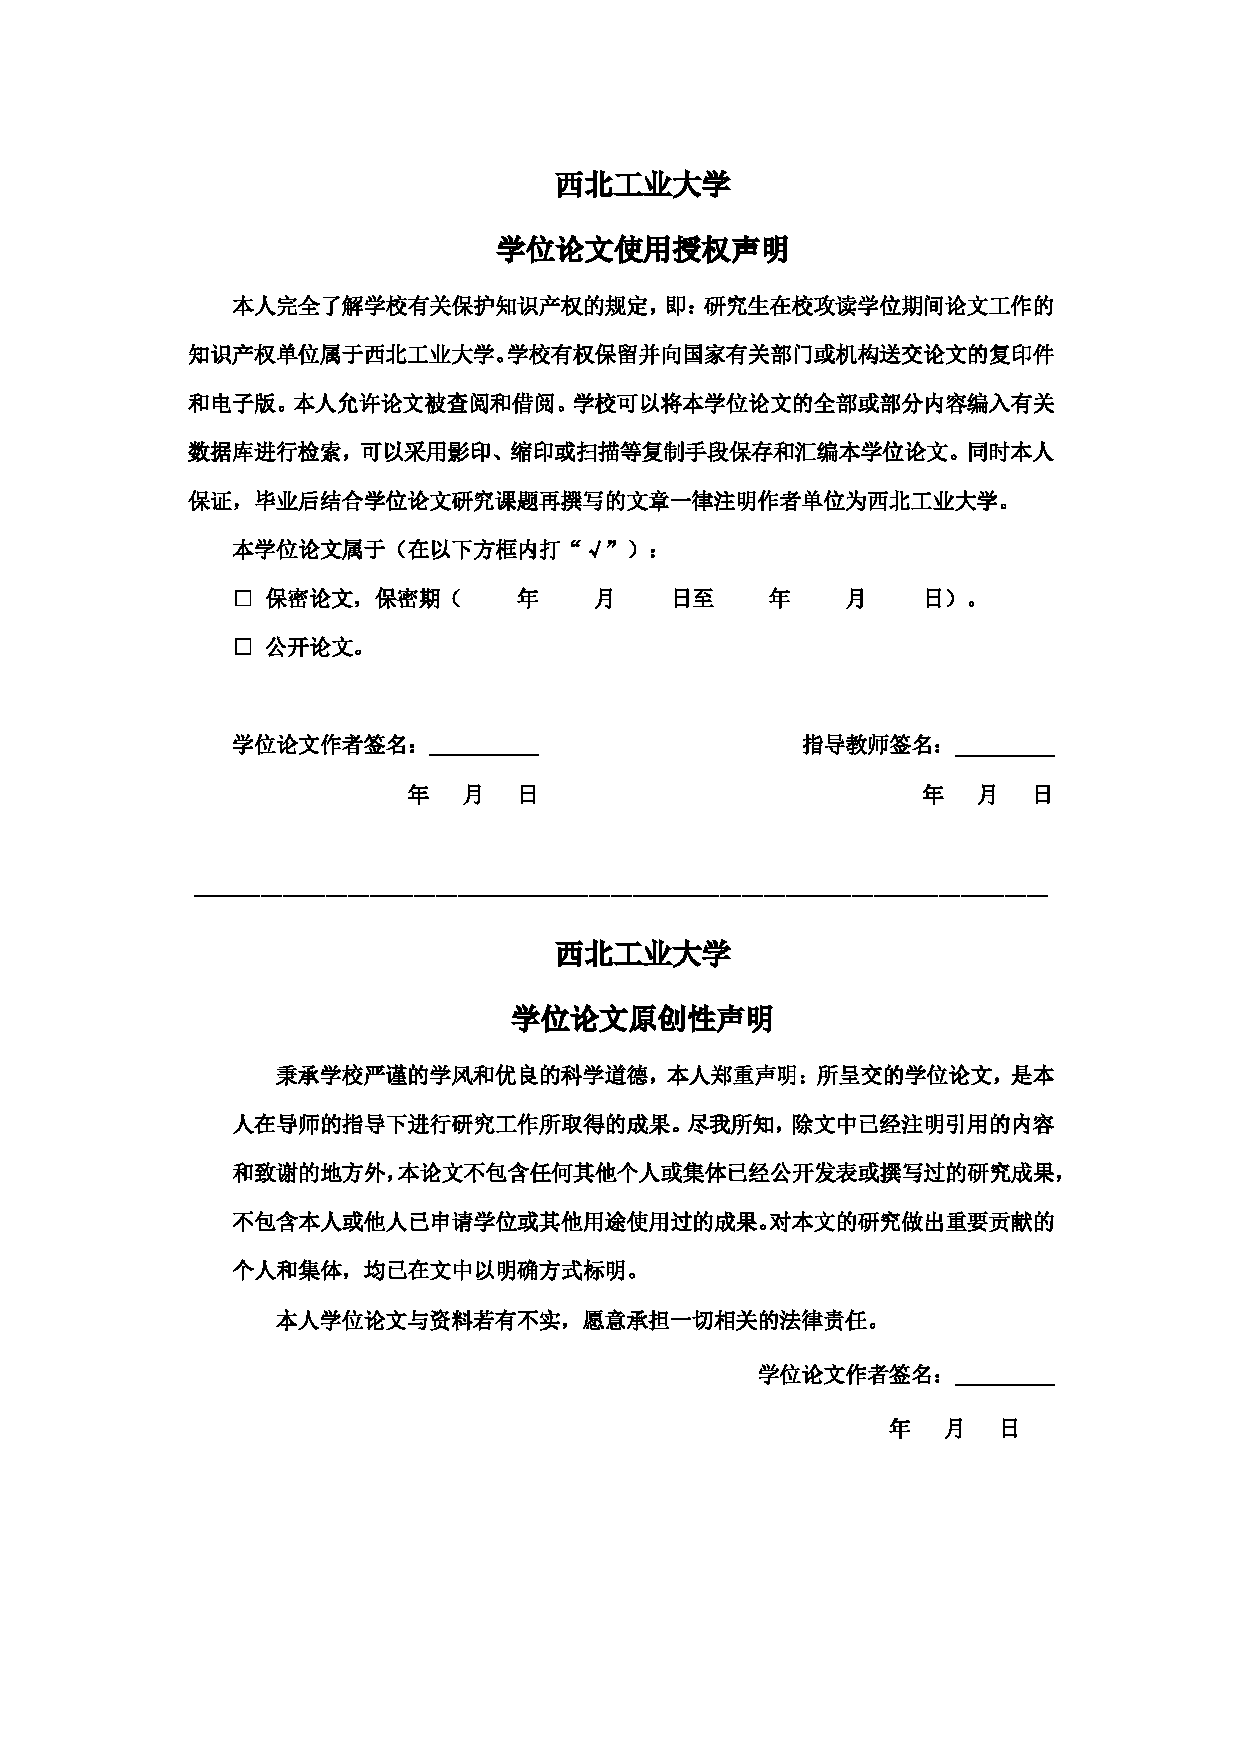
\includepdf[pages=-]{content/figures/研究生学位论文使用授权声明.pdf}

\end{document}

